\subsection{Neutral Meson Fitting Result}
\subsubsection{\texorpdfstring{Crystal Ball Fitting of $\pi^0$ for all kinematic bins}{Crystal Ball Fitting of pi0 for all kinematic bins}}
\label{sec:cryfitpi0}
\begin{figure}[H]
  \centering     
  \subfigure[$z$ bin 0, $0.1<z<0.2$]{\label{fig:pi0fitz1}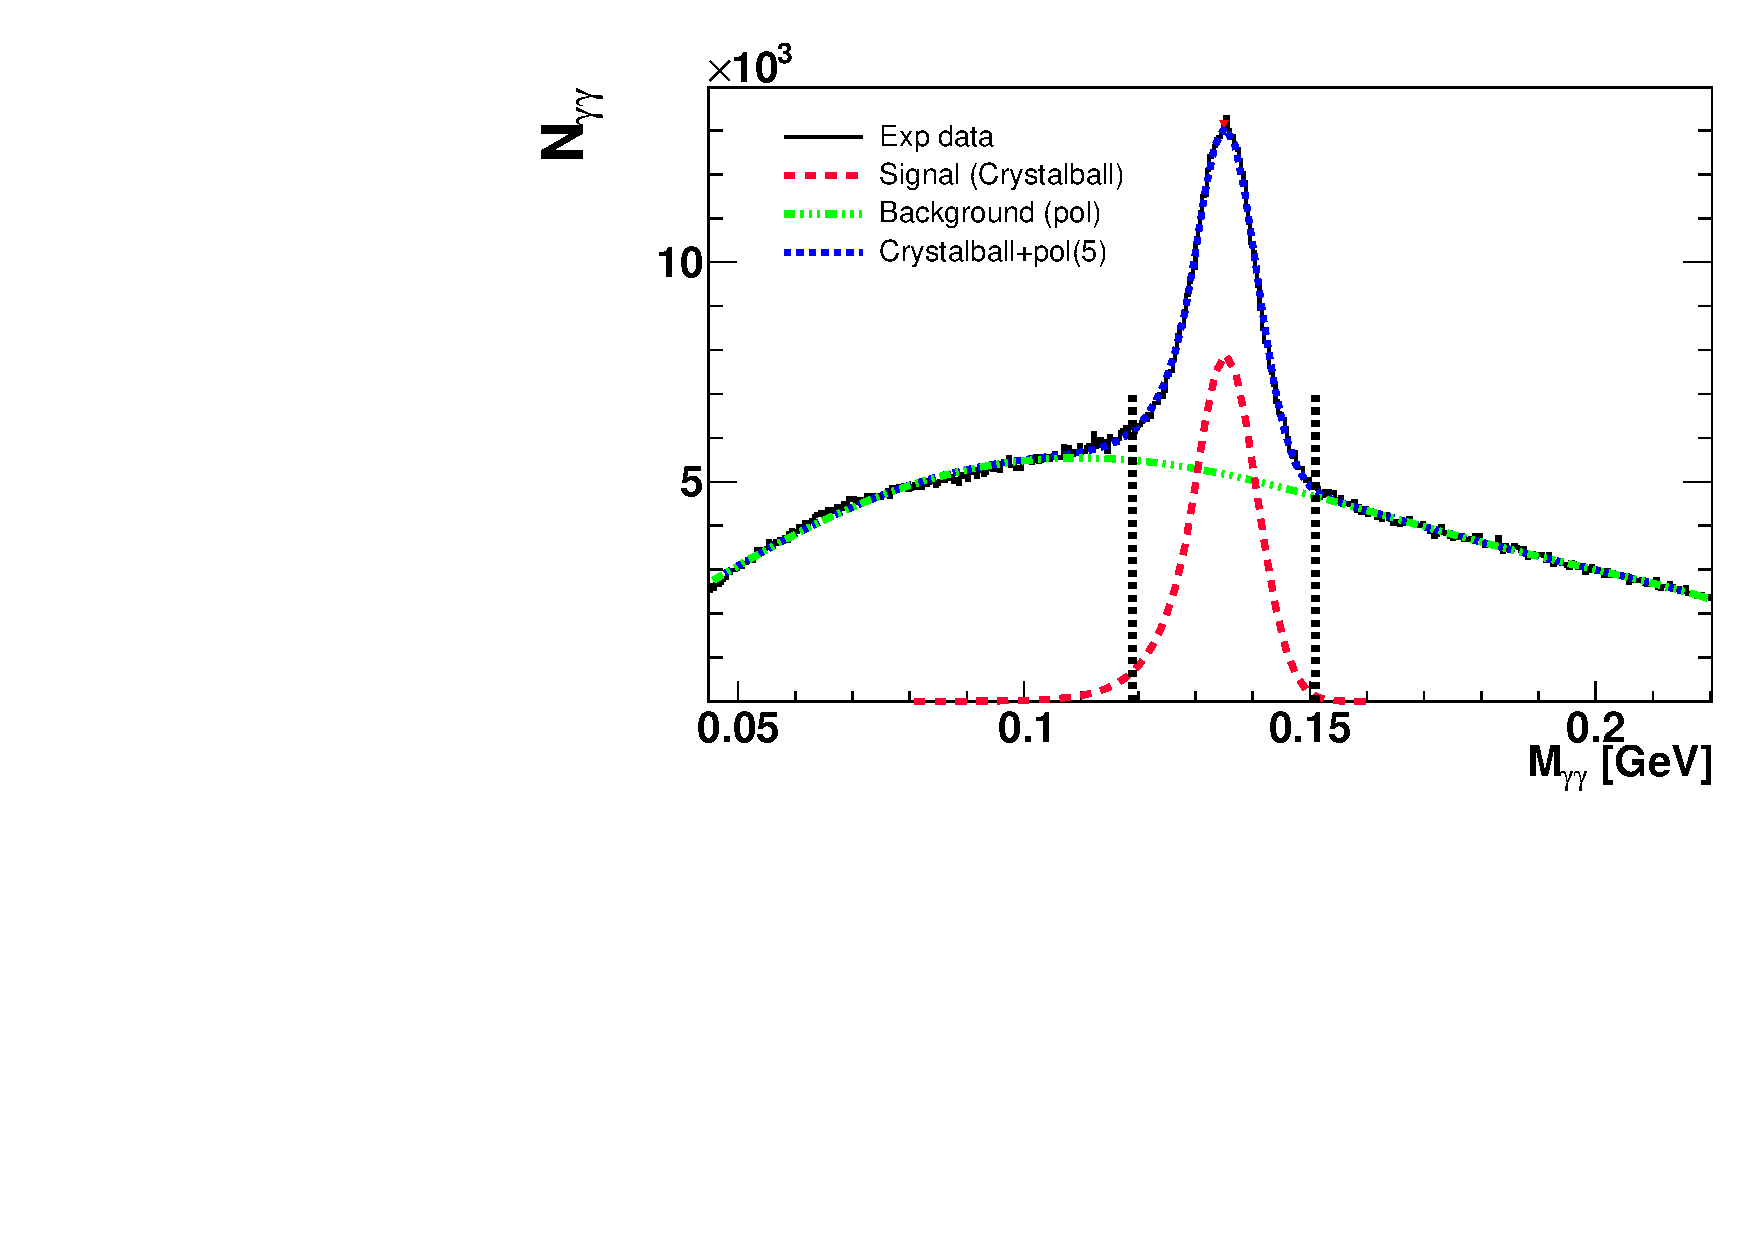
\includegraphics[width=.48\textwidth,natwidth=600,natheight=400]{figure_dataselection/pi0_crystalfit_Z_0.pdf}}
  \subfigure[$z$ bin 1, $0.2<z<0.3$]{\label{fig:pi0fitz2}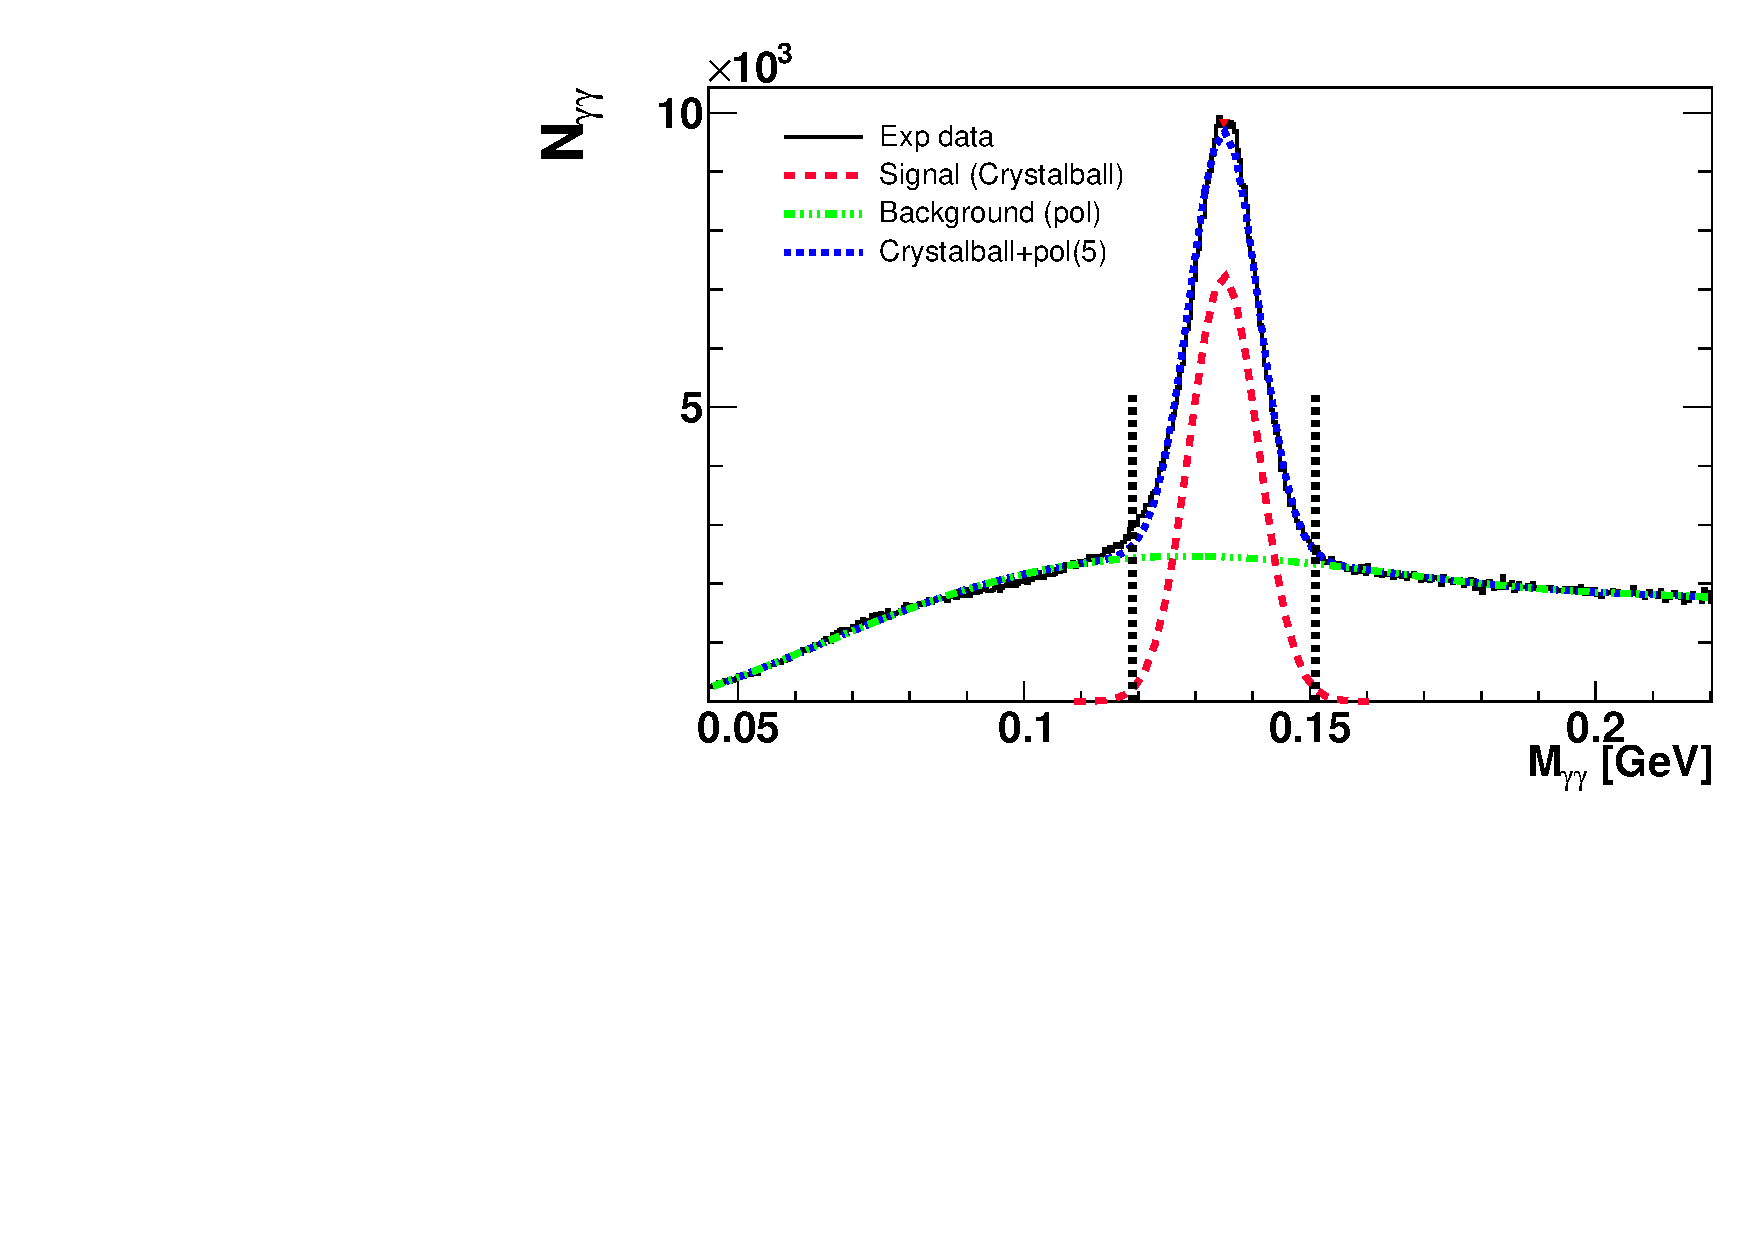
\includegraphics[width=.48\textwidth,natwidth=600,natheight=400]{figure_dataselection/pi0_crystalfit_Z_1.pdf}}
  \subfigure[$z$ bin 2, $0.3<z<0.4$]{\label{fig:pi0fitz3}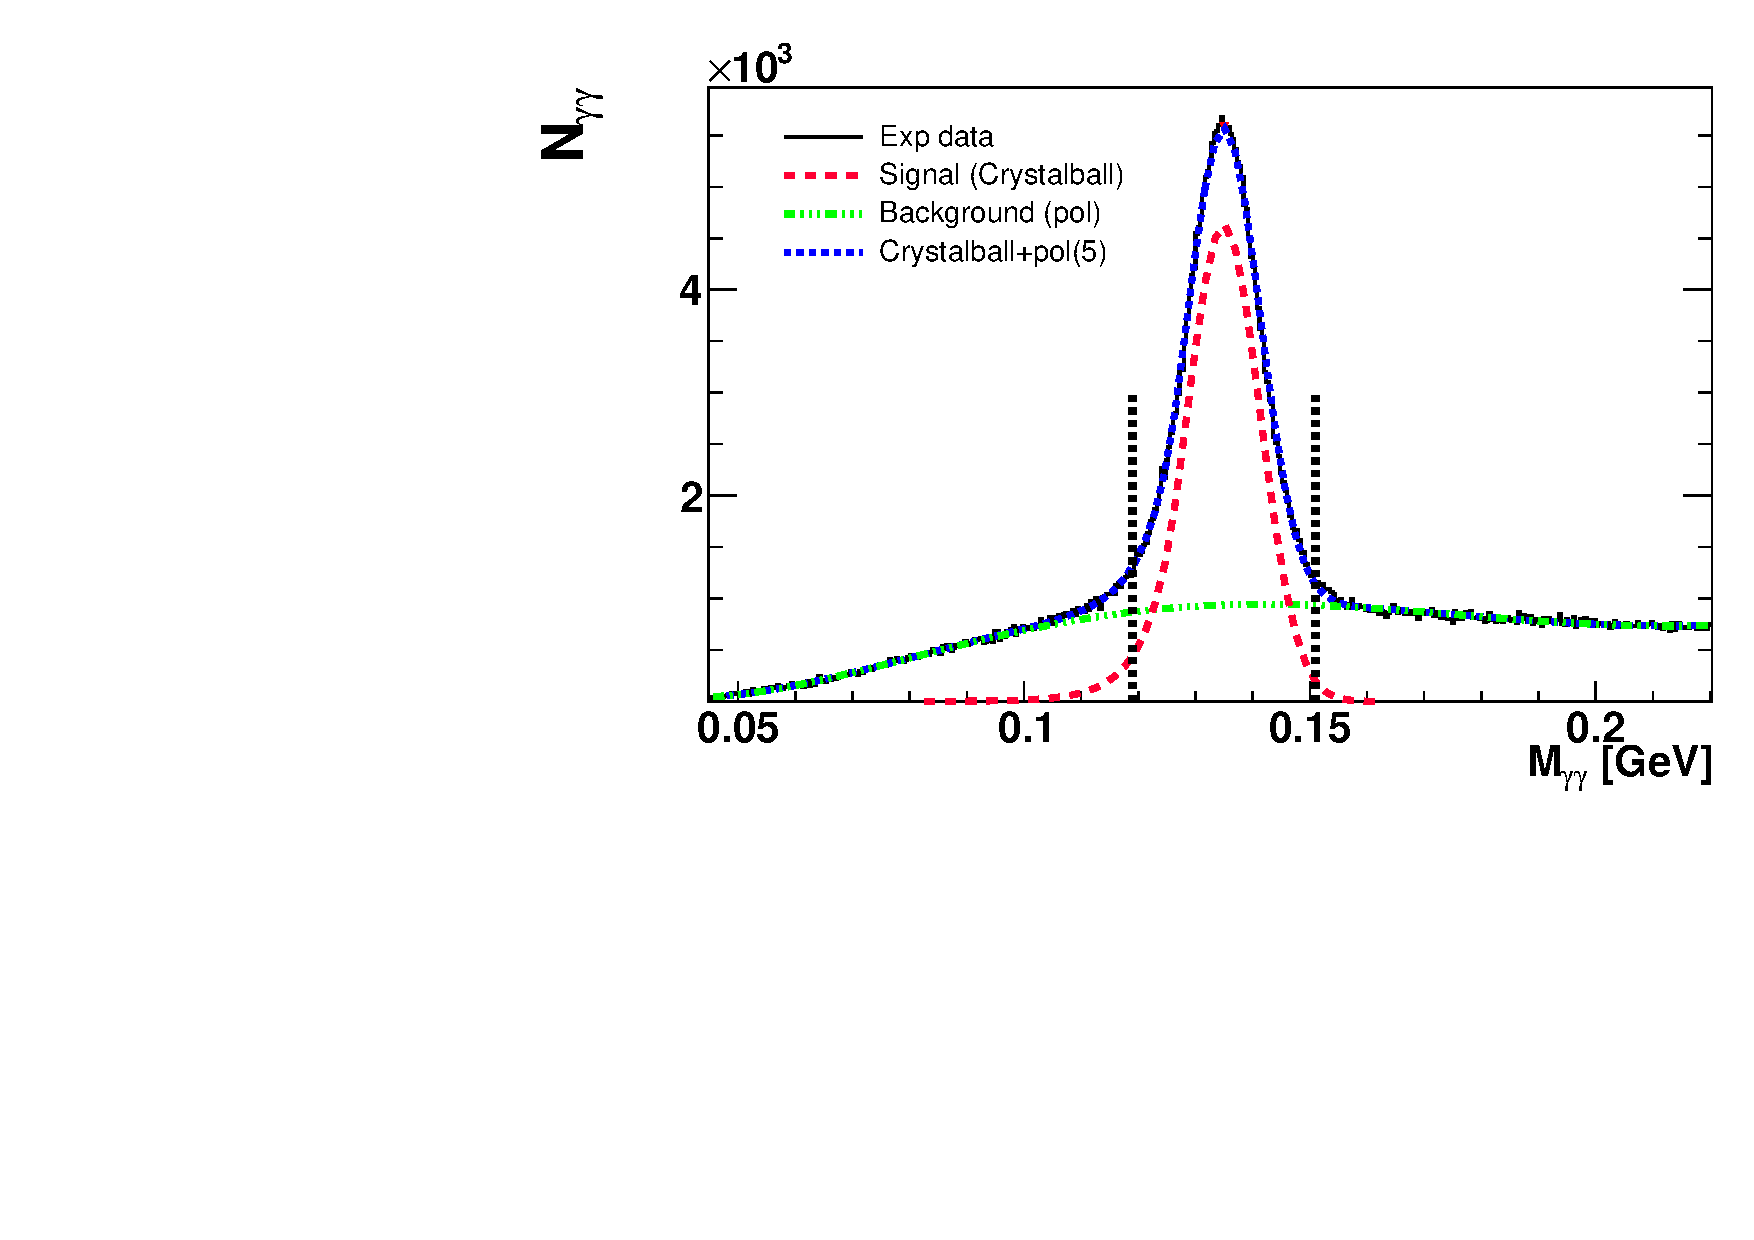
\includegraphics[width=.48\textwidth,natwidth=600,natheight=400]{figure_dataselection/pi0_crystalfit_Z_2.pdf}}
  \subfigure[$z$ bin 3, $0.4<z<0.5$]{\label{fig:pi0fitz4}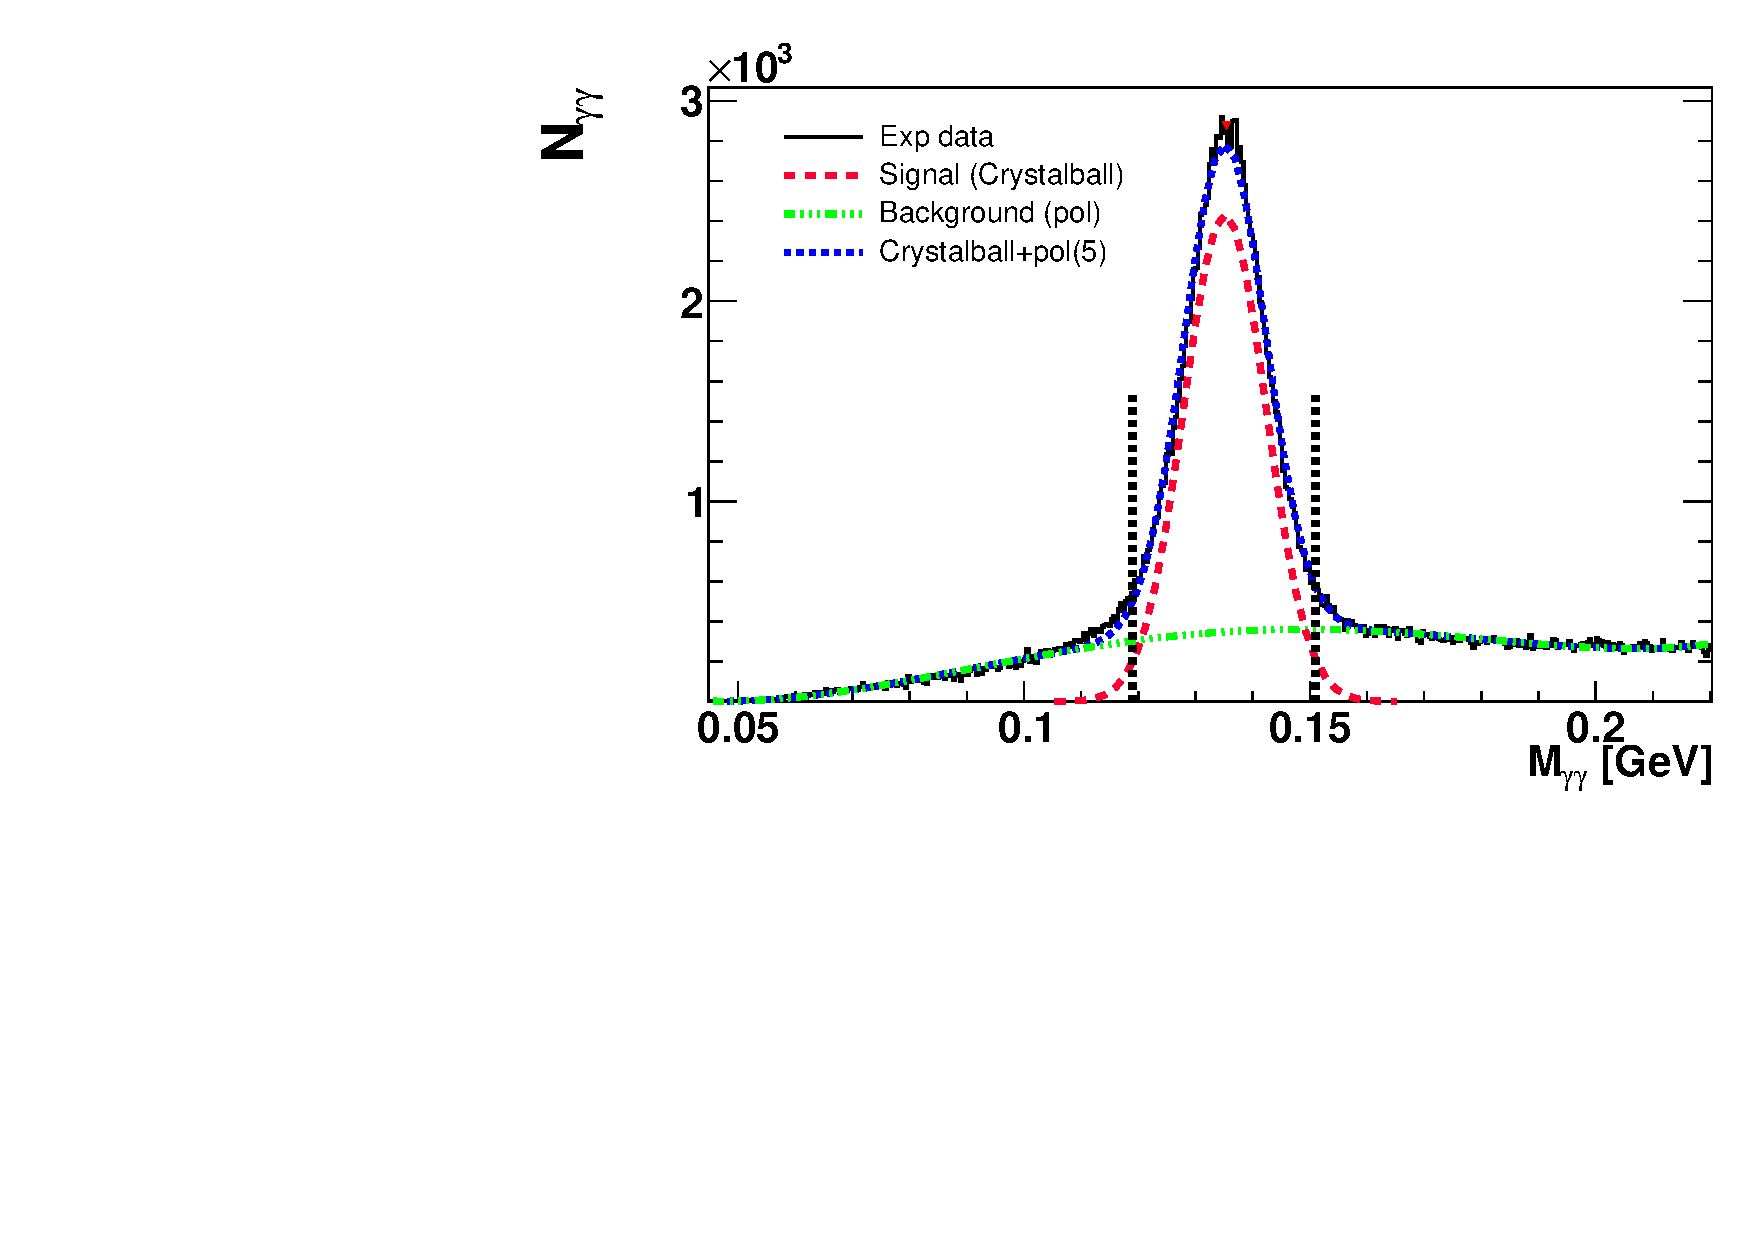
\includegraphics[width=.48\textwidth,natwidth=600,natheight=400]{figure_dataselection/pi0_crystalfit_Z_3.pdf}}
  \subfigure[$z$ bin 4, $0.5<z<0.6$]{\label{fig:pi0fitz5}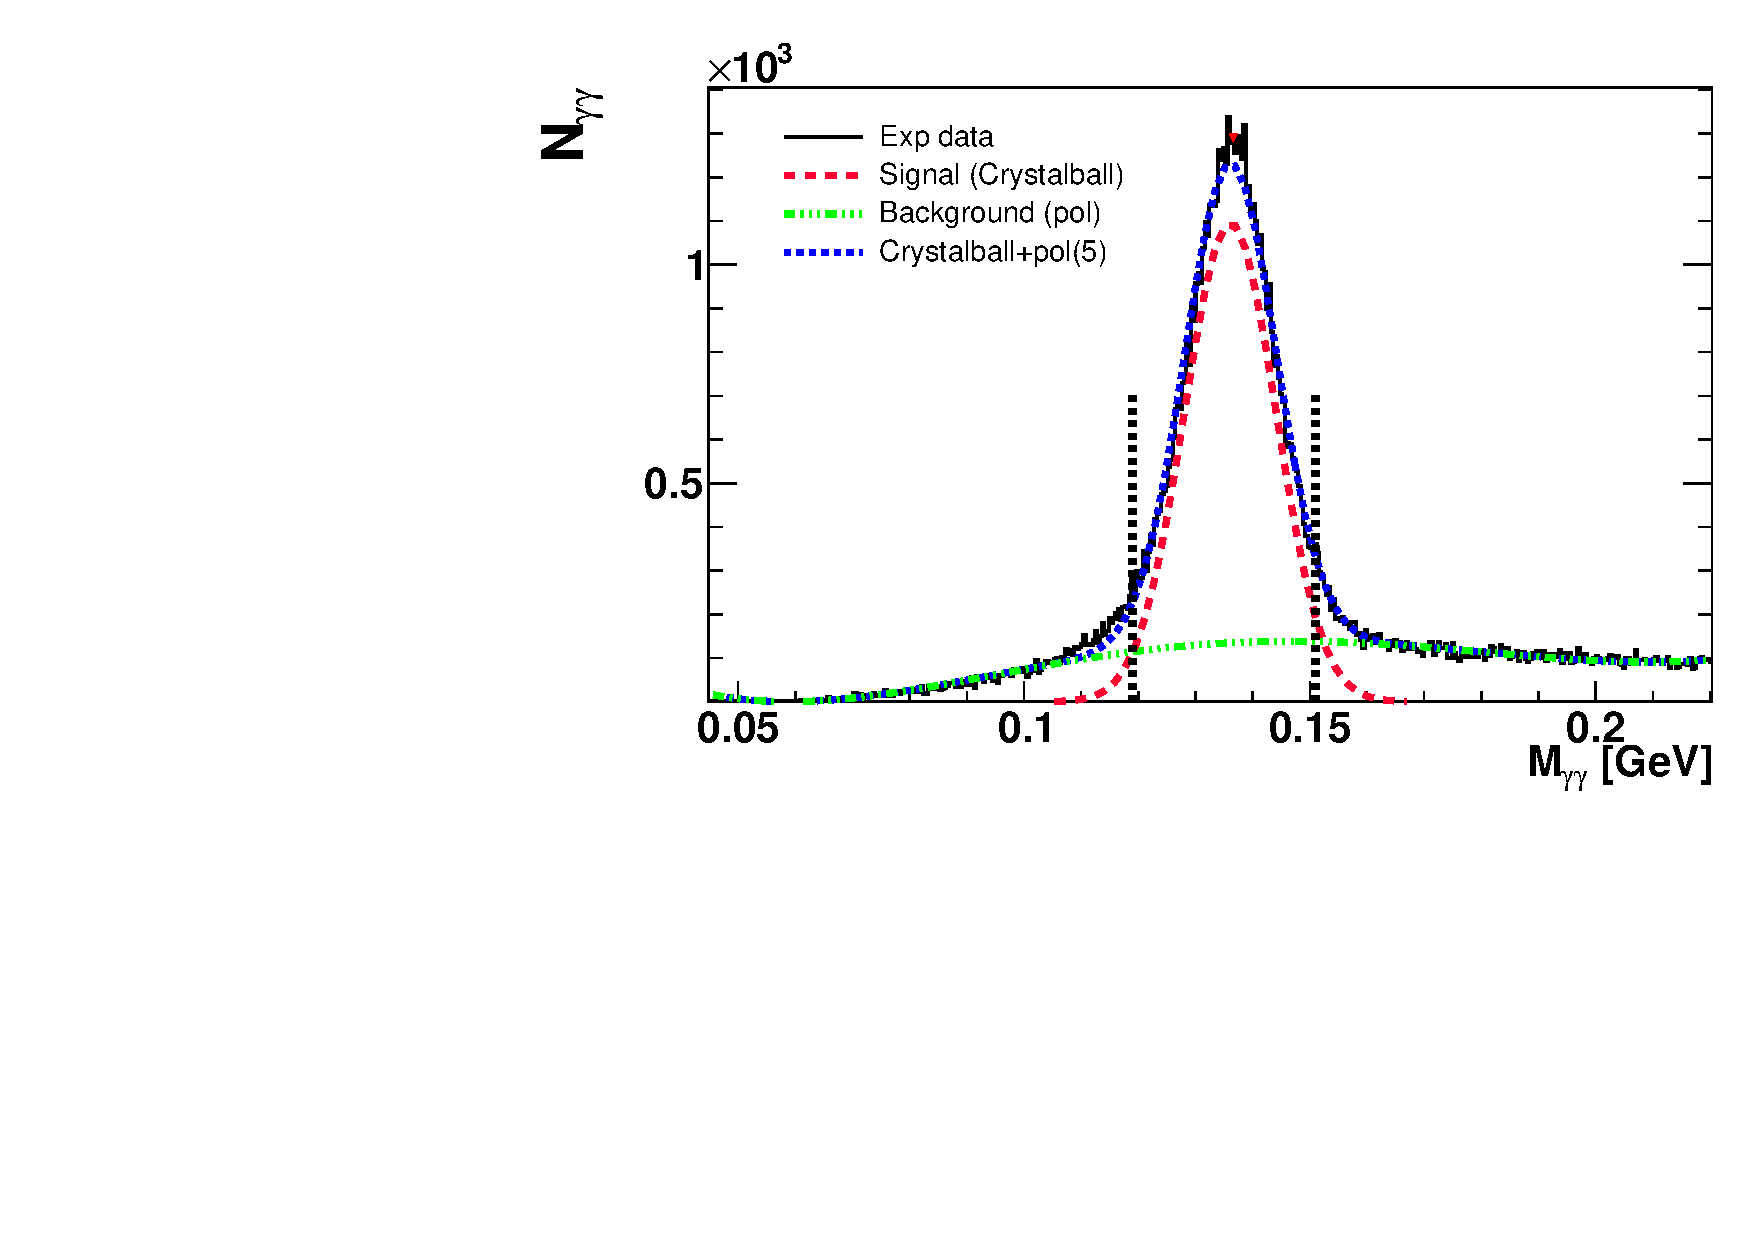
\includegraphics[width=.48\textwidth,natwidth=600,natheight=400]{figure_dataselection/pi0_crystalfit_Z_4.pdf}}
  \subfigure[$z$ bin 5, $0.6<z<0.7$]{\label{fig:pi0fitz6}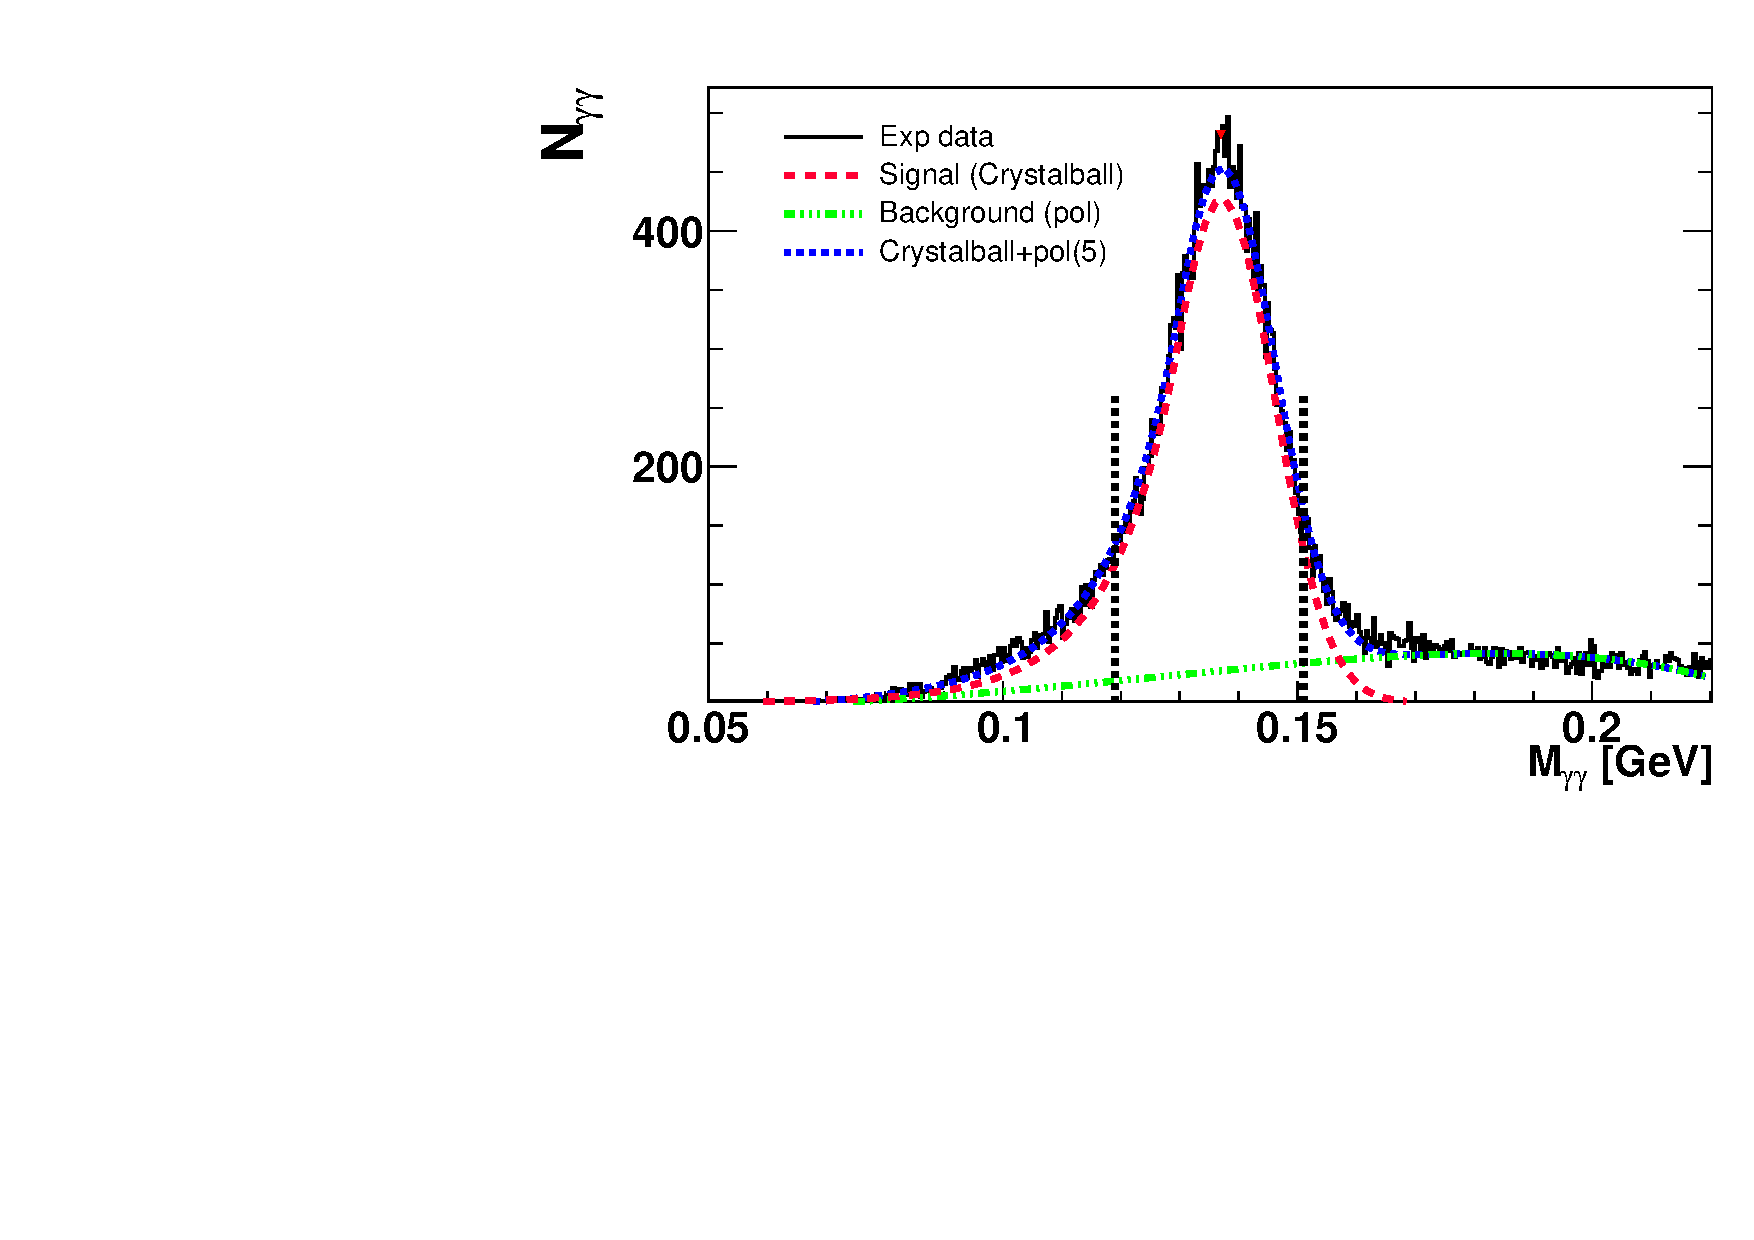
\includegraphics[width=.48\textwidth,natwidth=600,natheight=400]{figure_dataselection/pi0_crystalfit_Z_5.pdf}}
  \subfigure[$z$ bin 6, $0.7<z<1$]{\label{fig:pi0fitz7}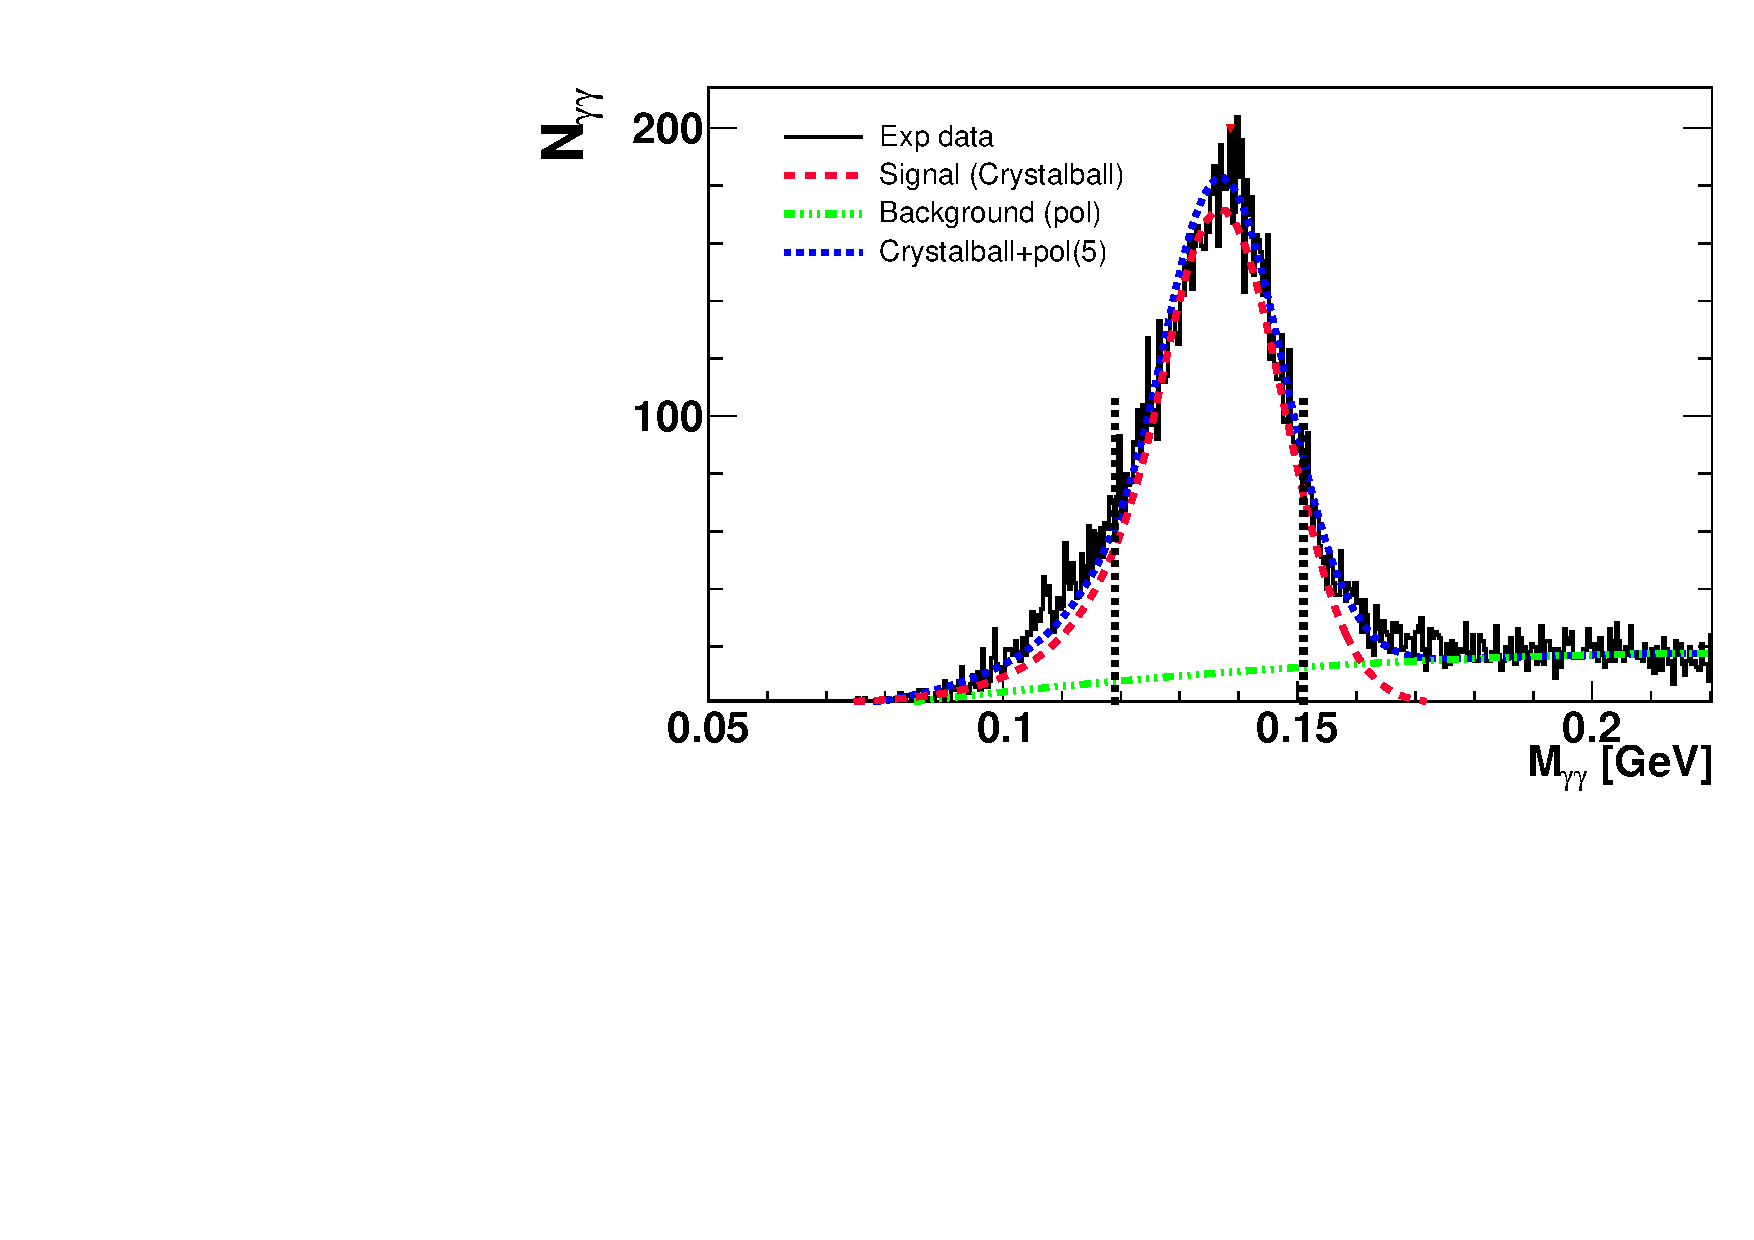
\includegraphics[width=.48\textwidth,natwidth=600,natheight=400]{figure_dataselection/pi0_crystalfit_Z_6.pdf}}
\label{fig:pi0zfit}
\caption{}
\end{figure}

\begin{figure}[H]
 \ContinuedFloat 
  \centering
  \subfigure[$P_t$ bin 1, $0<p_t<0.15$]{\label{fig:pi0fitpt0}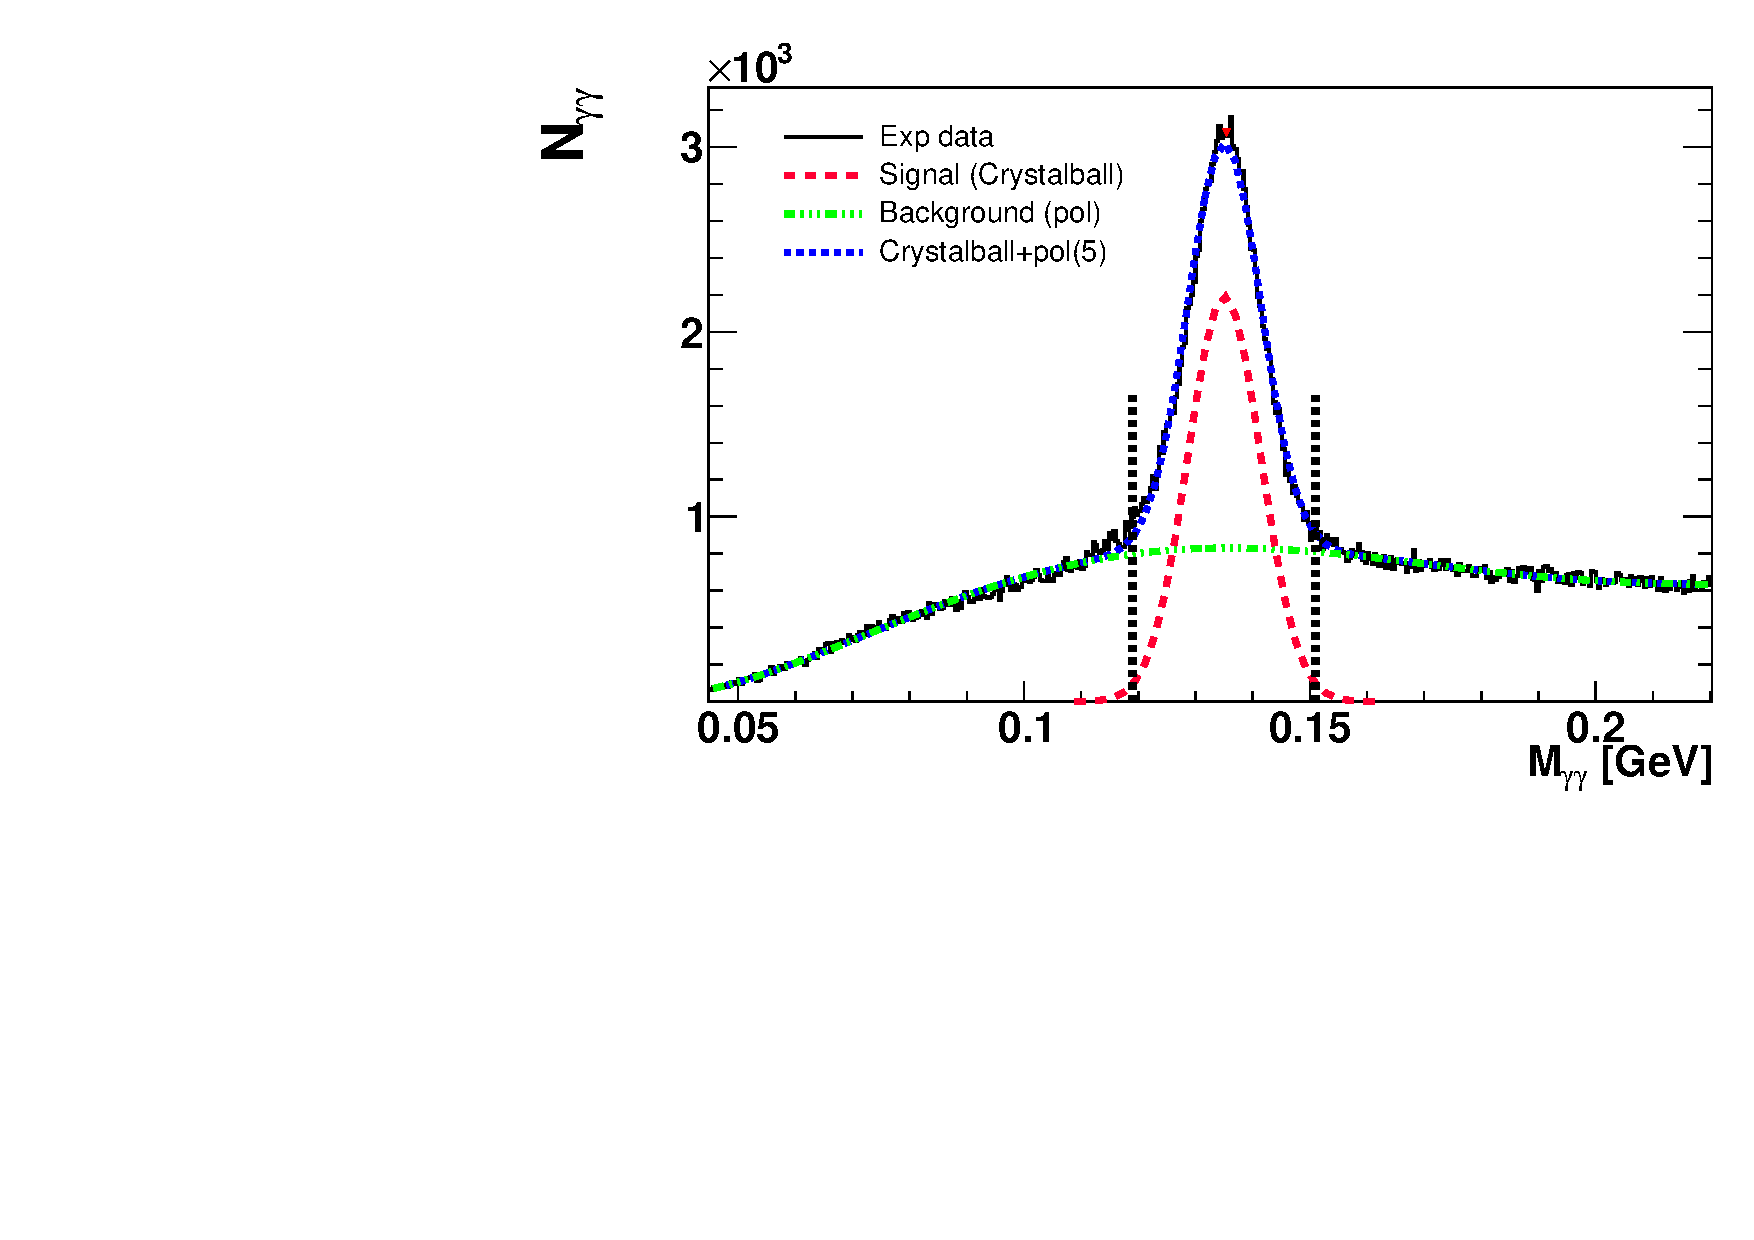
\includegraphics[width=.48\textwidth,natwidth=600,natheight=400]{figure_dataselection/pi0_crystalfit_Pt_0.pdf}}
  \subfigure[$P_t$ bin 2, $0.15<p_t<0.3$]{\label{fig:pi0fitpt1}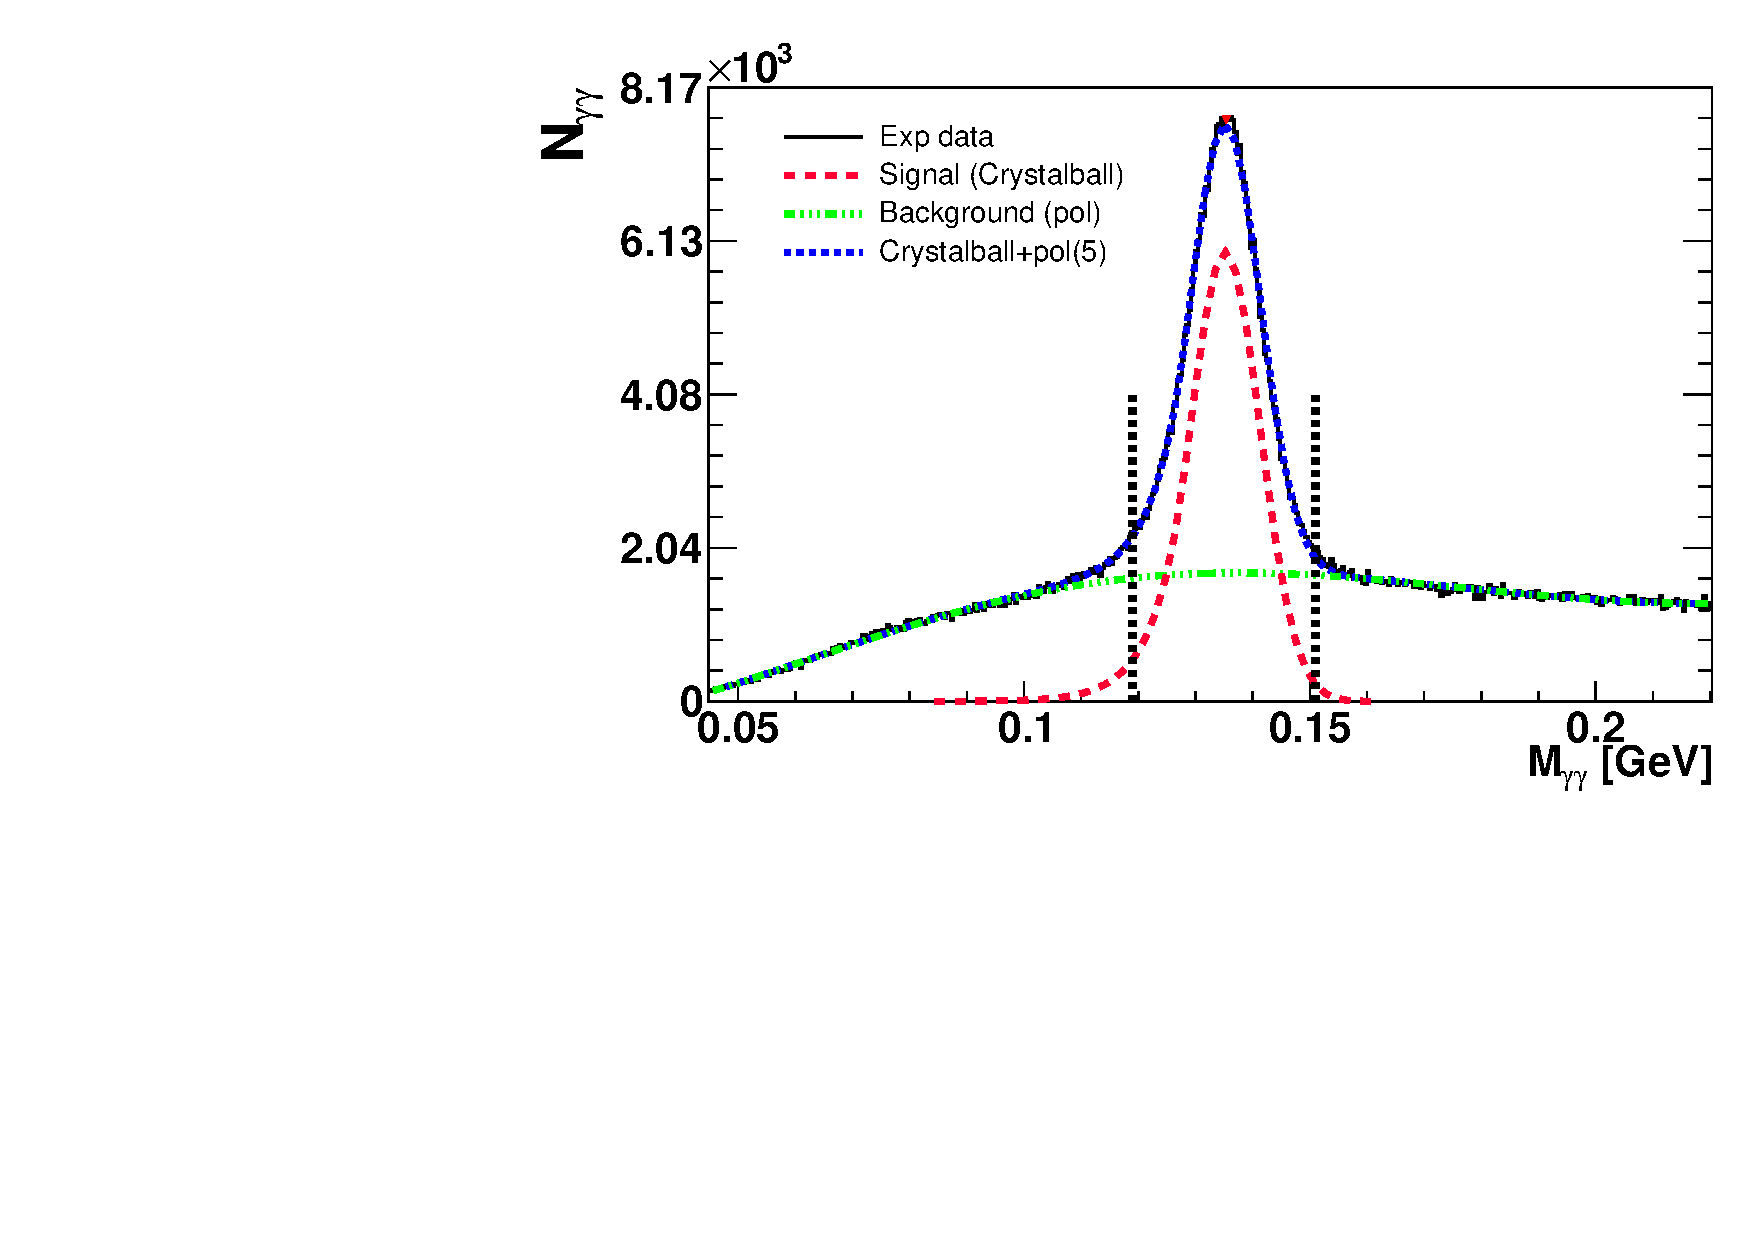
\includegraphics[width=.48\textwidth,natwidth=600,natheight=400]{figure_dataselection/pi0_crystalfit_Pt_1.pdf}}
  \subfigure[$P_t$ bin 3, $0.3<p_t<0.5$]{\label{fig:pi0fitpt2}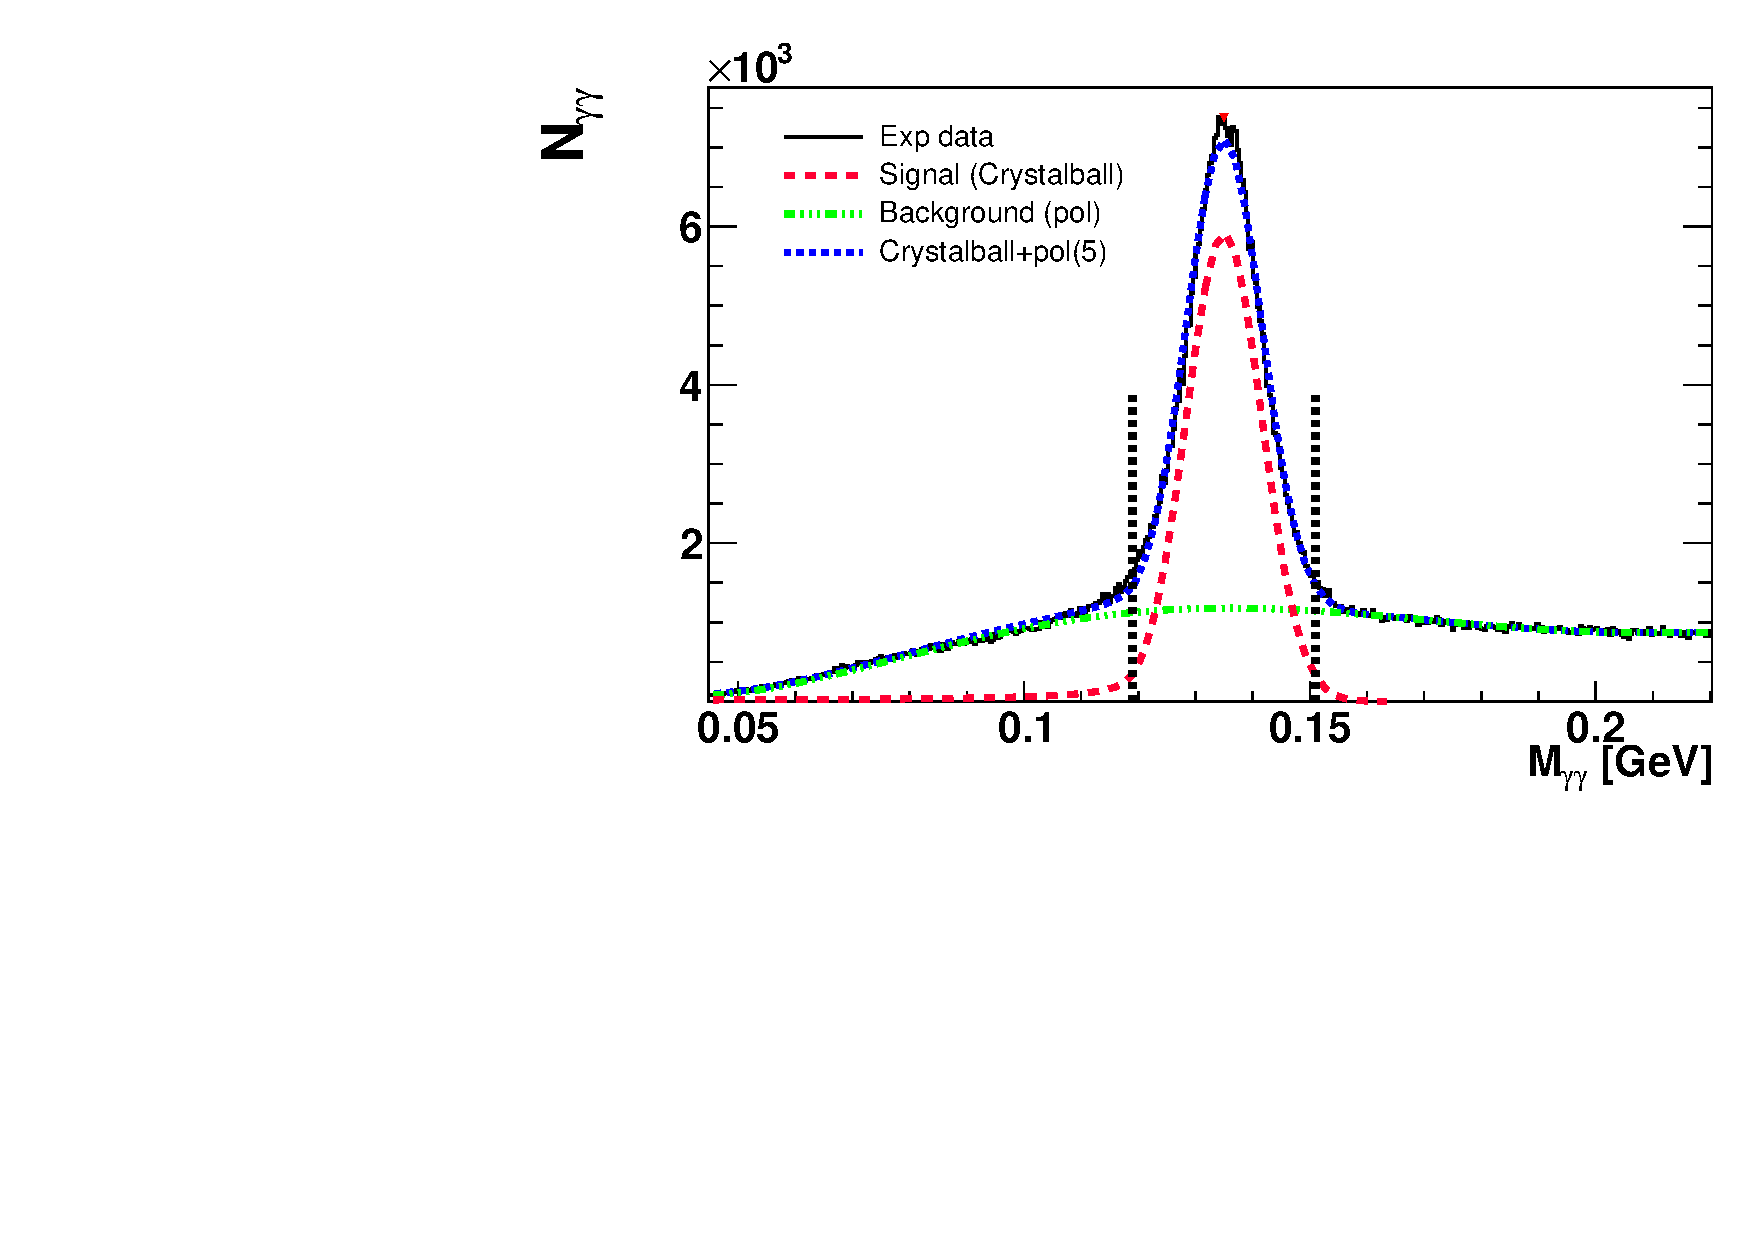
\includegraphics[width=.48\textwidth,natwidth=600,natheight=400]{figure_dataselection/pi0_crystalfit_Pt_2.pdf}}
  \subfigure[$P_t$ bin 4, $0.5<p_t<3$]{\label{fig:pi0fitpt3}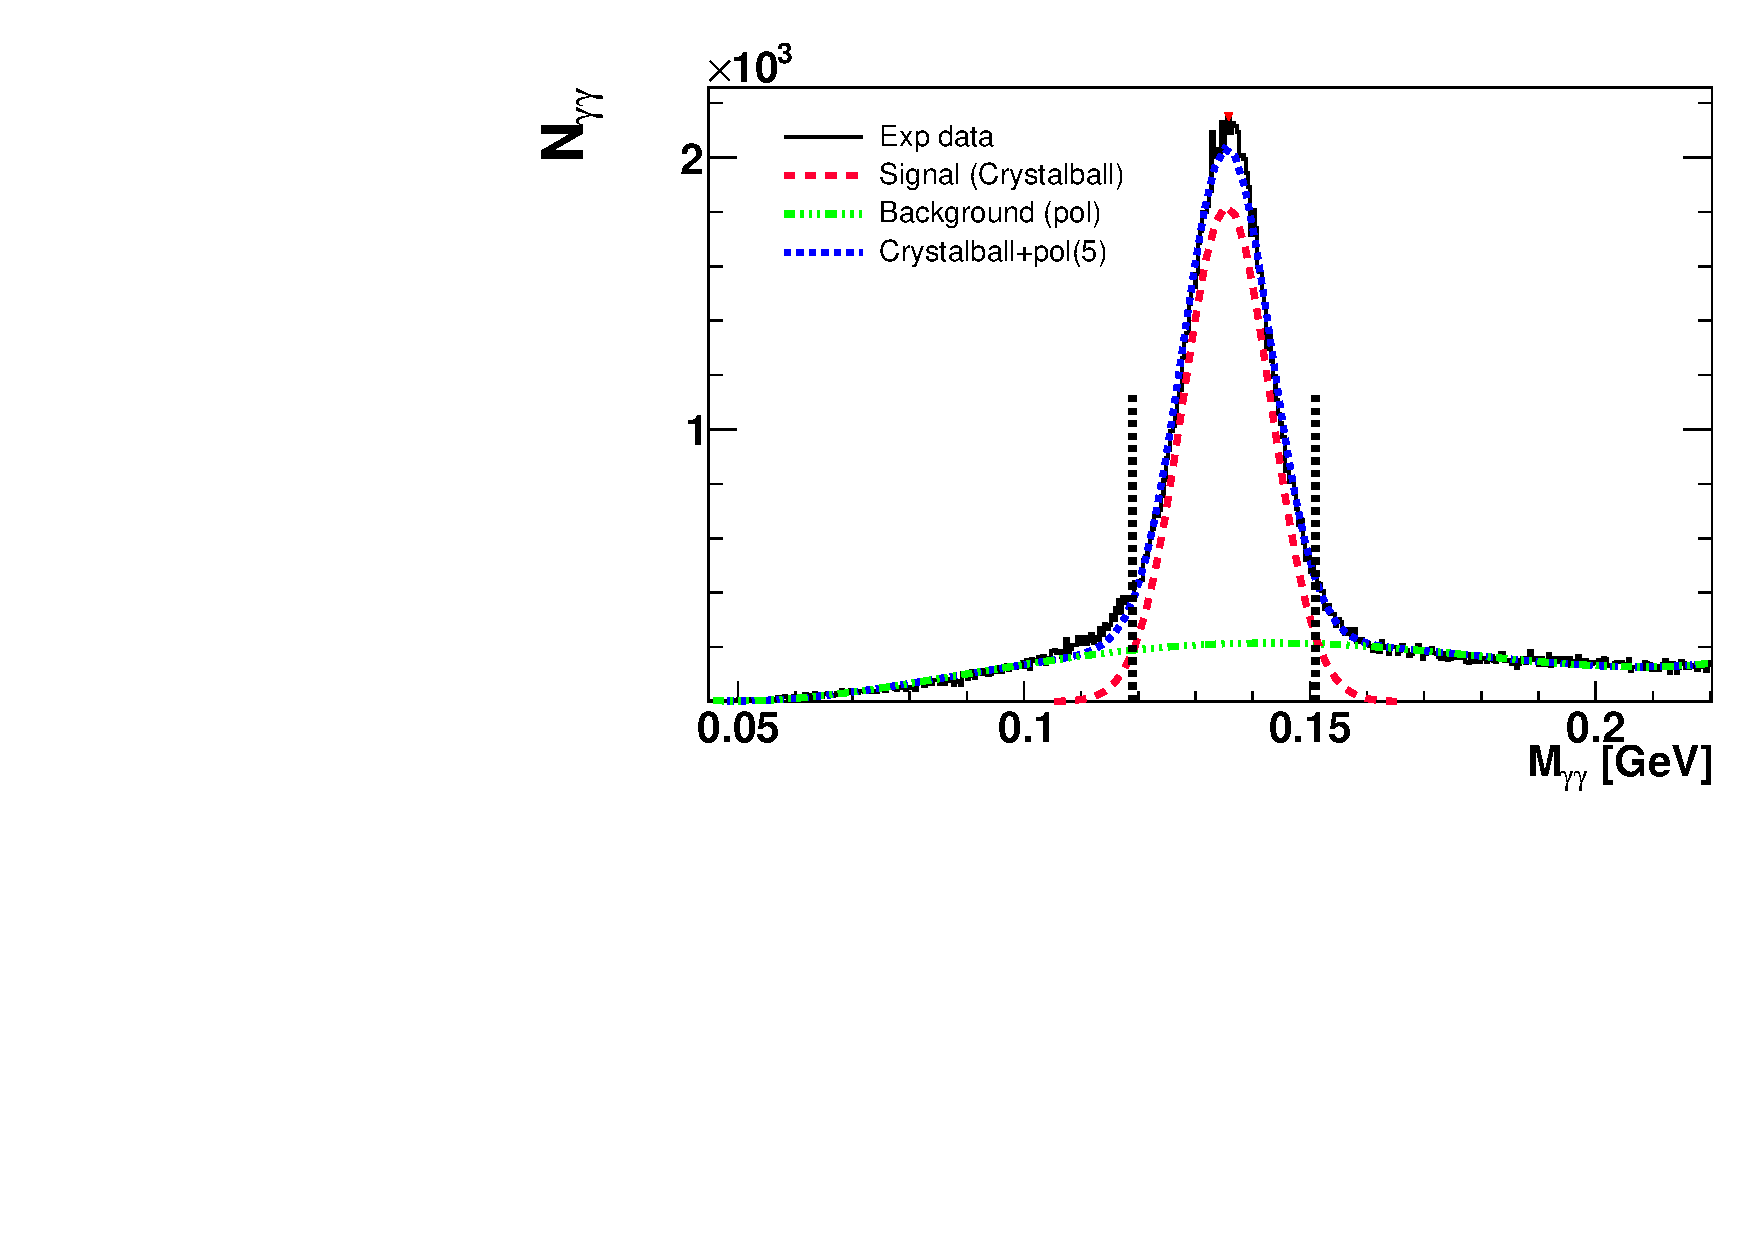
\includegraphics[width=.48\textwidth,natwidth=600,natheight=400]{figure_dataselection/pi0_crystalfit_Pt_3.pdf}}
  \caption{$\pi^0$ fit results for all kinematic bins. Fit method has described in section~\ref{sec:pi0fitsection}. Red line is the background and green line is the signal.}
  \label{fig:pi0ptfit}
\end{figure}

\subsubsection{\texorpdfstring{Fit with MC Background of $\pi^0$ for all kinematic bins}{Fit with MC Background of pi0 for all kinematic bins}}
\label{sec:bkgfitpi0}
\begin{figure}[H]
  \centering     
  \subfigure[$z$ bin 0, $0.1<z<0.2$]{\label{fig:pi0fitz1}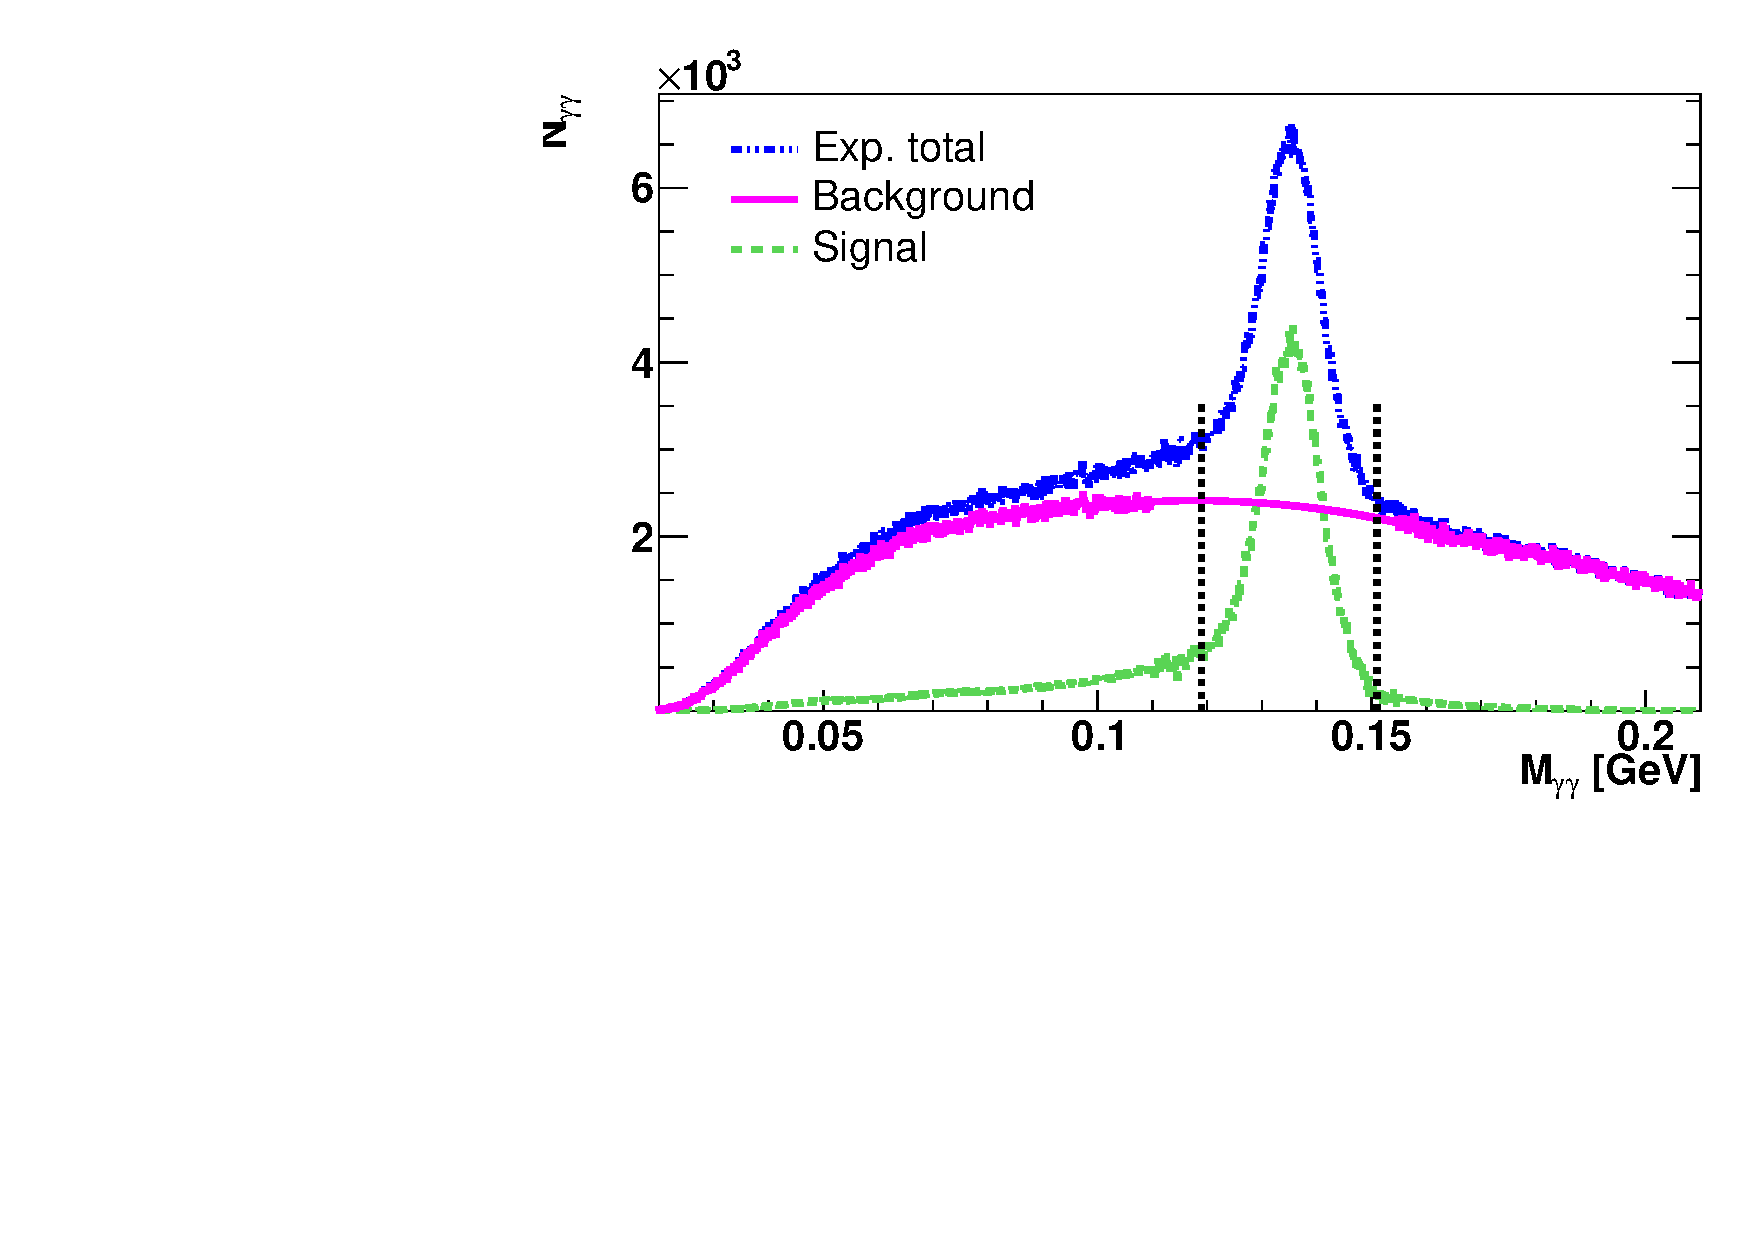
\includegraphics[width=.48\textwidth,natwidth=600,natheight=400]{figure_dataselection/pi0_fit_Z_0.pdf}}
  \subfigure[$z$ bin 1, $0.2<z<0.3$]{\label{fig:pi0fitz2}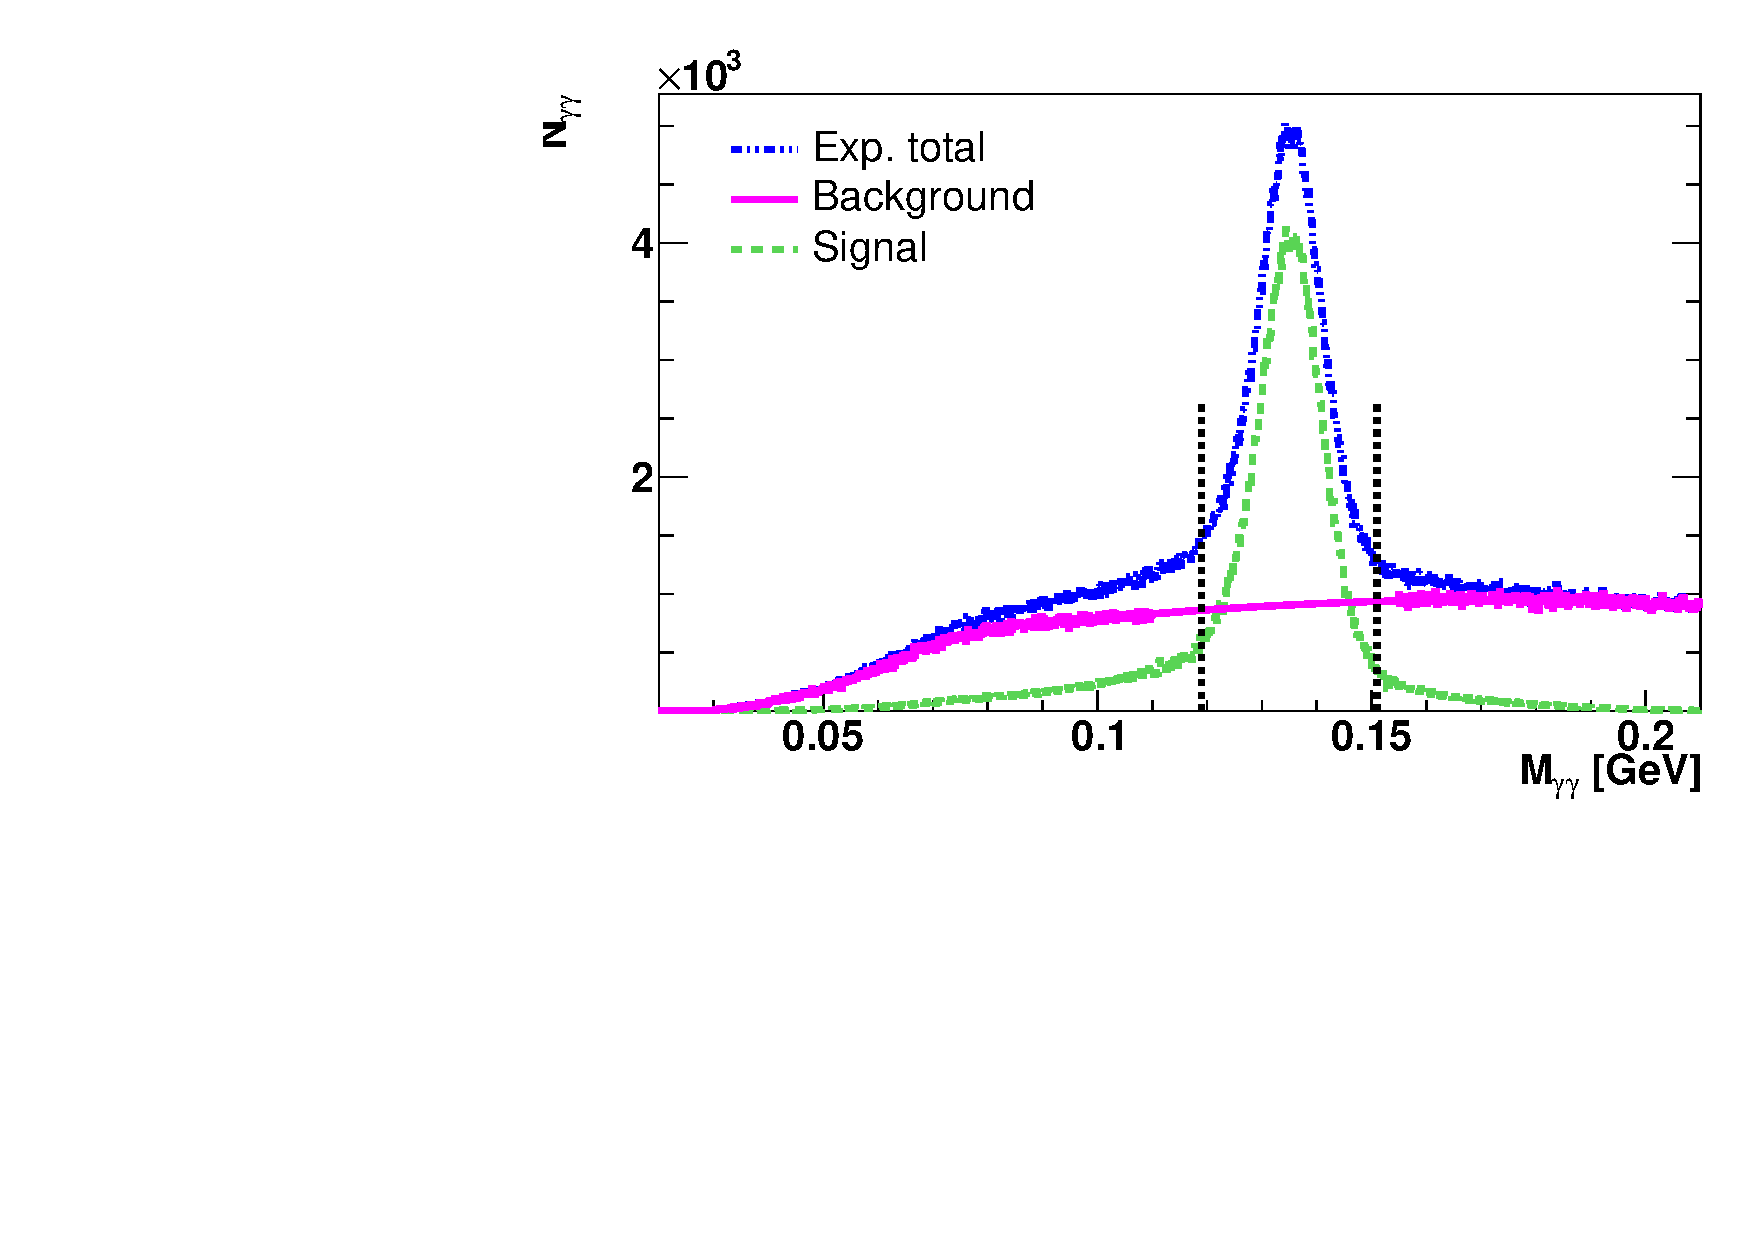
\includegraphics[width=.48\textwidth,natwidth=600,natheight=400]{figure_dataselection/pi0_fit_Z_1.pdf}}
  \subfigure[$z$ bin 2, $0.3<z<0.4$]{\label{fig:pi0fitz3}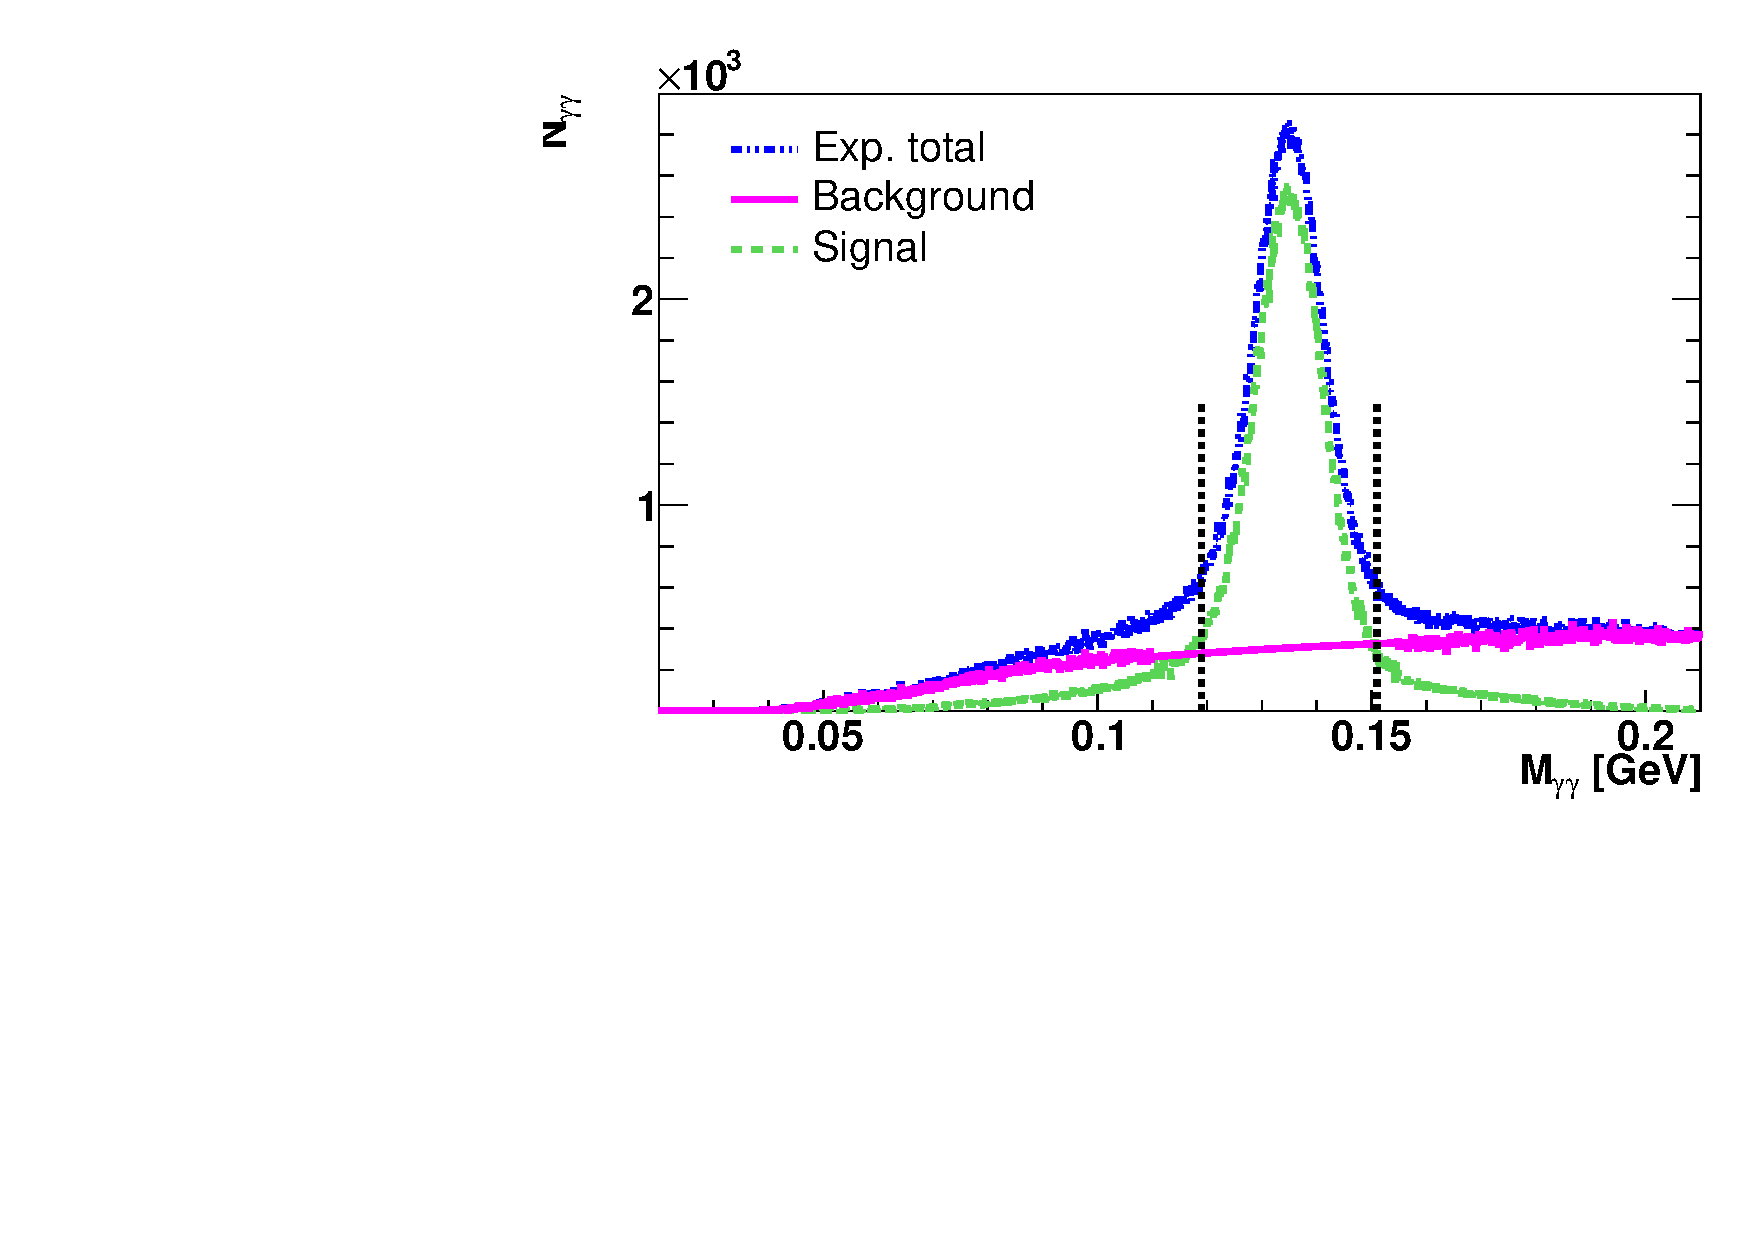
\includegraphics[width=.48\textwidth,natwidth=600,natheight=400]{figure_dataselection/pi0_fit_Z_2.pdf}}
  \subfigure[$z$ bin 3, $0.4<z<0.5$]{\label{fig:pi0fitz4}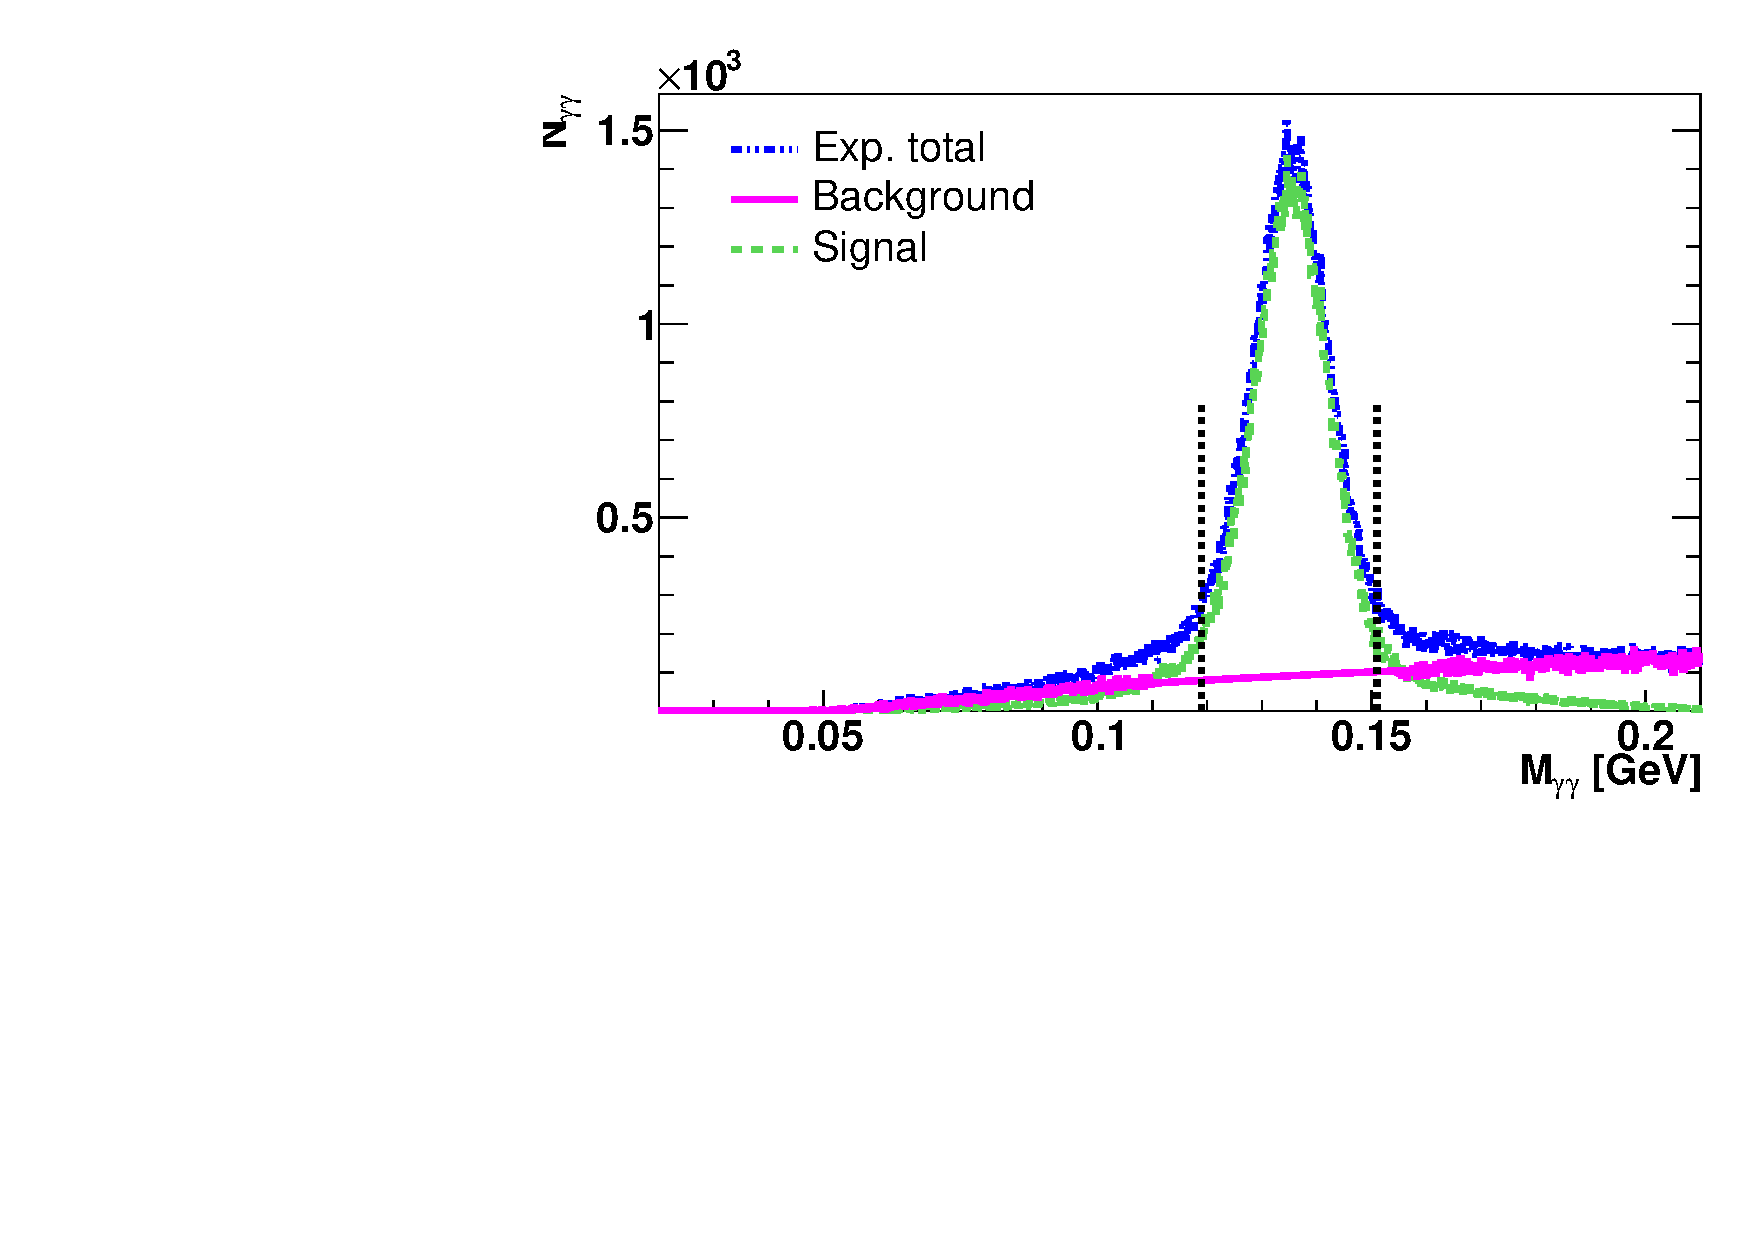
\includegraphics[width=.48\textwidth,natwidth=600,natheight=400]{figure_dataselection/pi0_fit_Z_3.pdf}}
  \subfigure[$z$ bin 4, $0.5<z<0.6$]{\label{fig:pi0fitz5}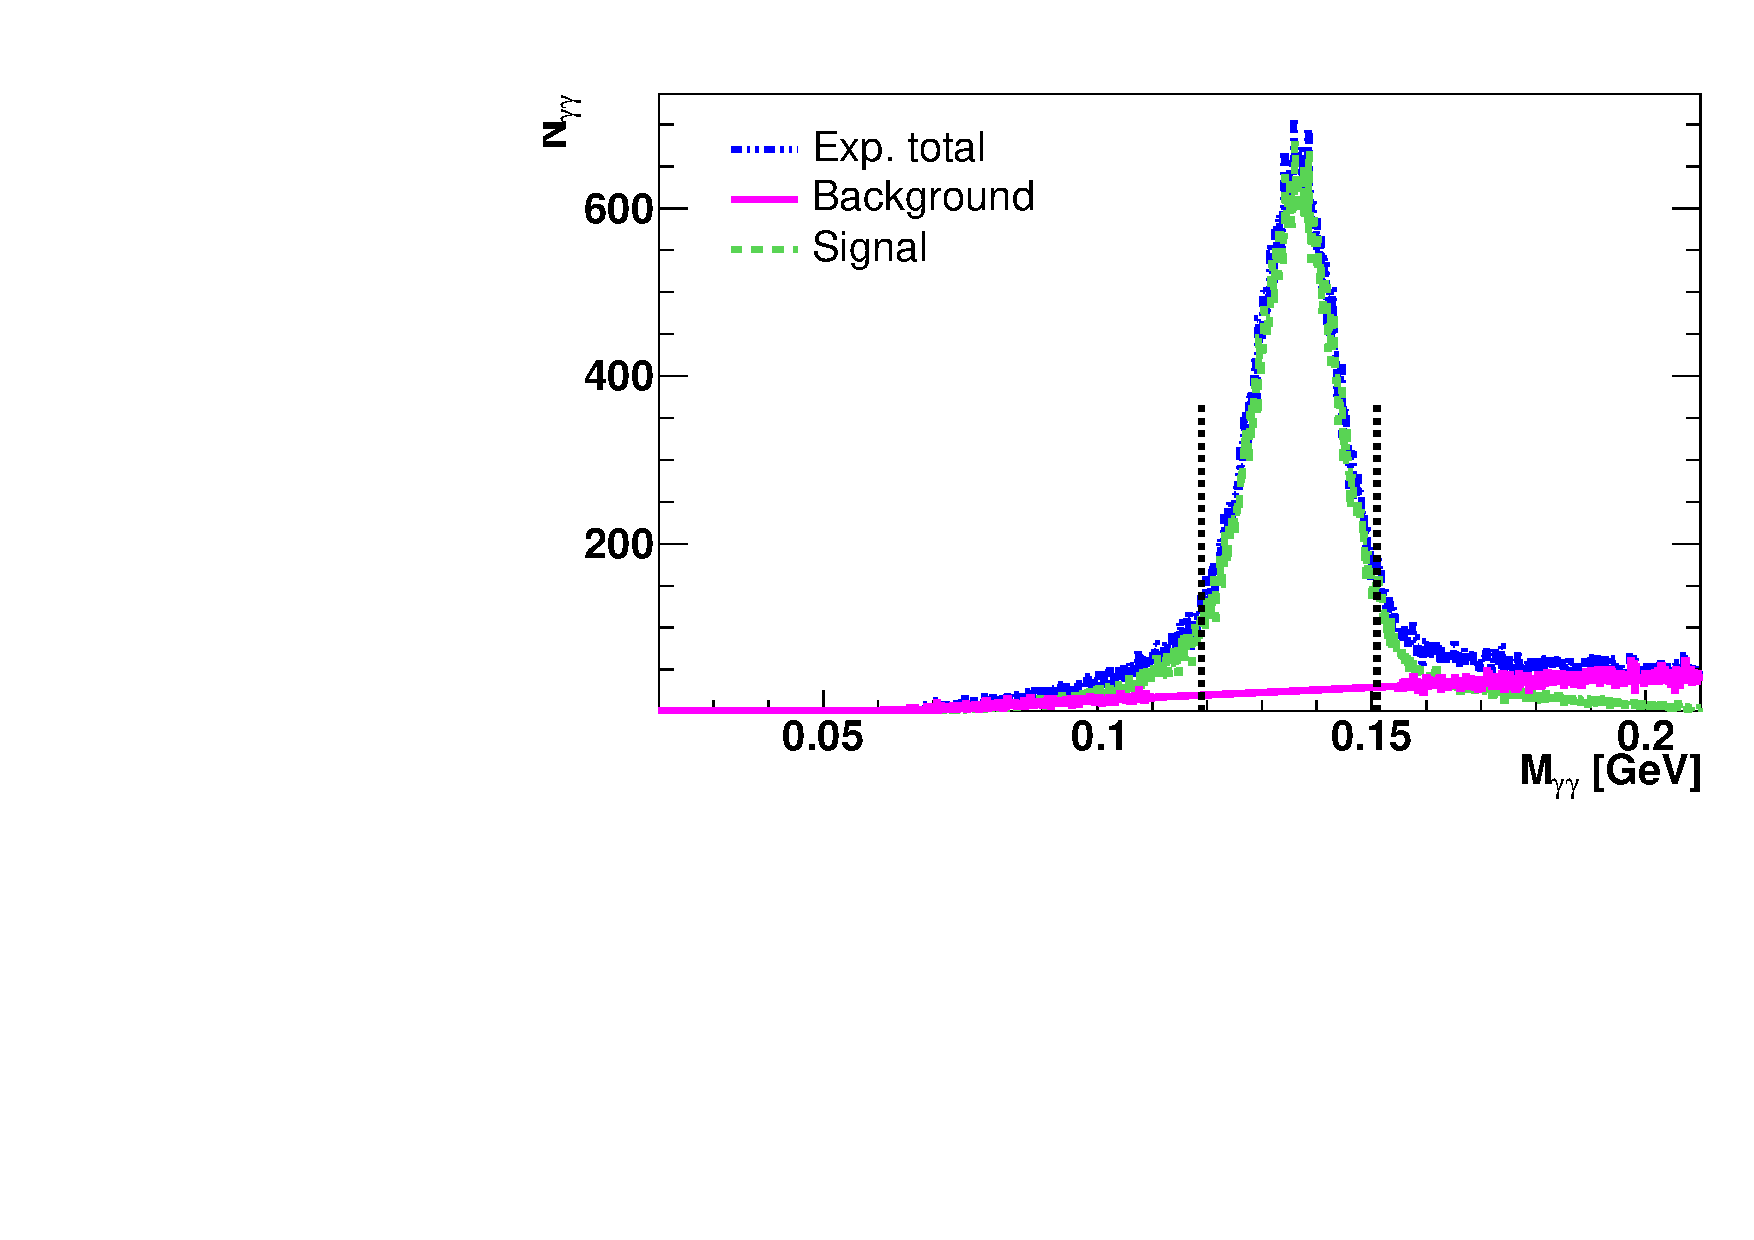
\includegraphics[width=.48\textwidth,natwidth=600,natheight=400]{figure_dataselection/pi0_fit_Z_4.pdf}}
  \subfigure[$z$ bin 5, $0.6<z<0.7$]{\label{fig:pi0fitz6}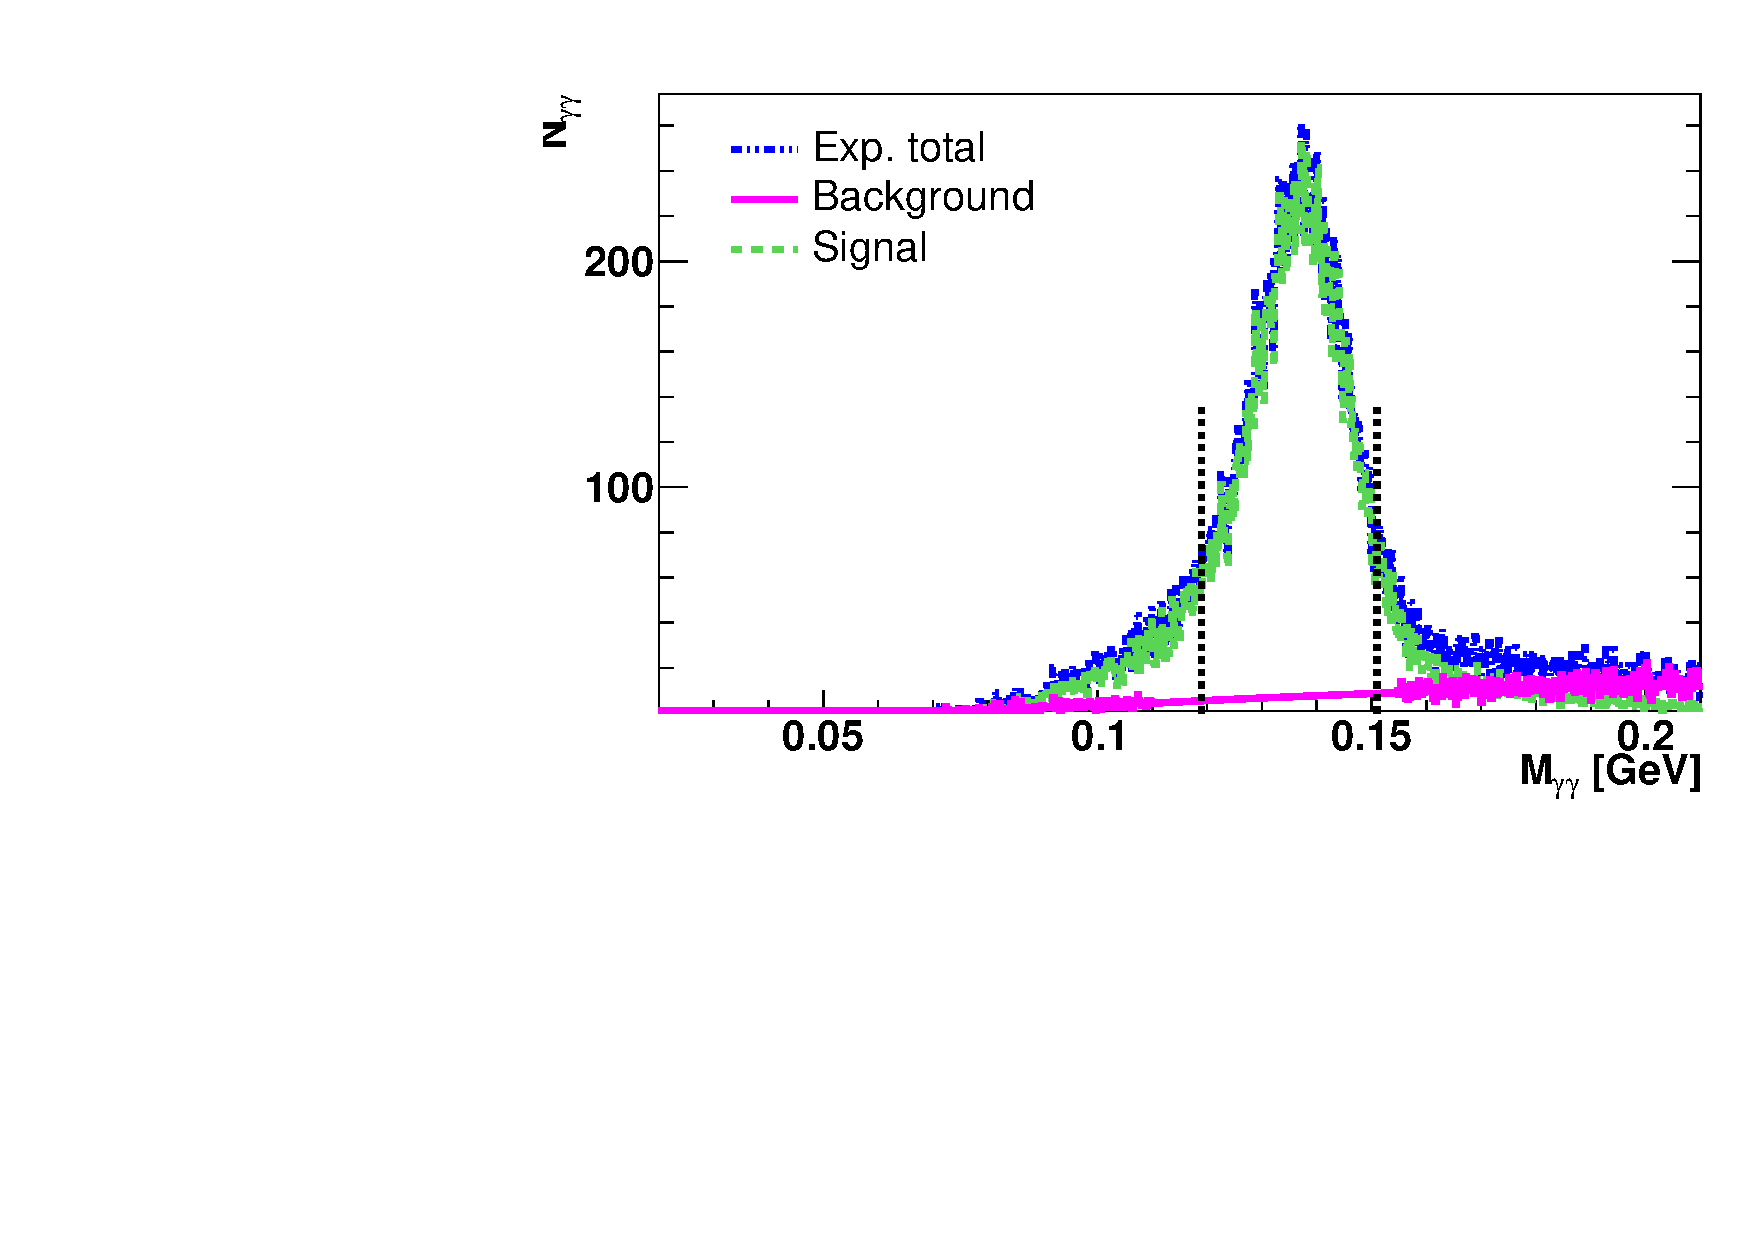
\includegraphics[width=.48\textwidth,natwidth=600,natheight=400]{figure_dataselection/pi0_fit_Z_5.pdf}}
  \subfigure[$z$ bin 6, $0.7<z<1$]{\label{fig:pi0fitz7}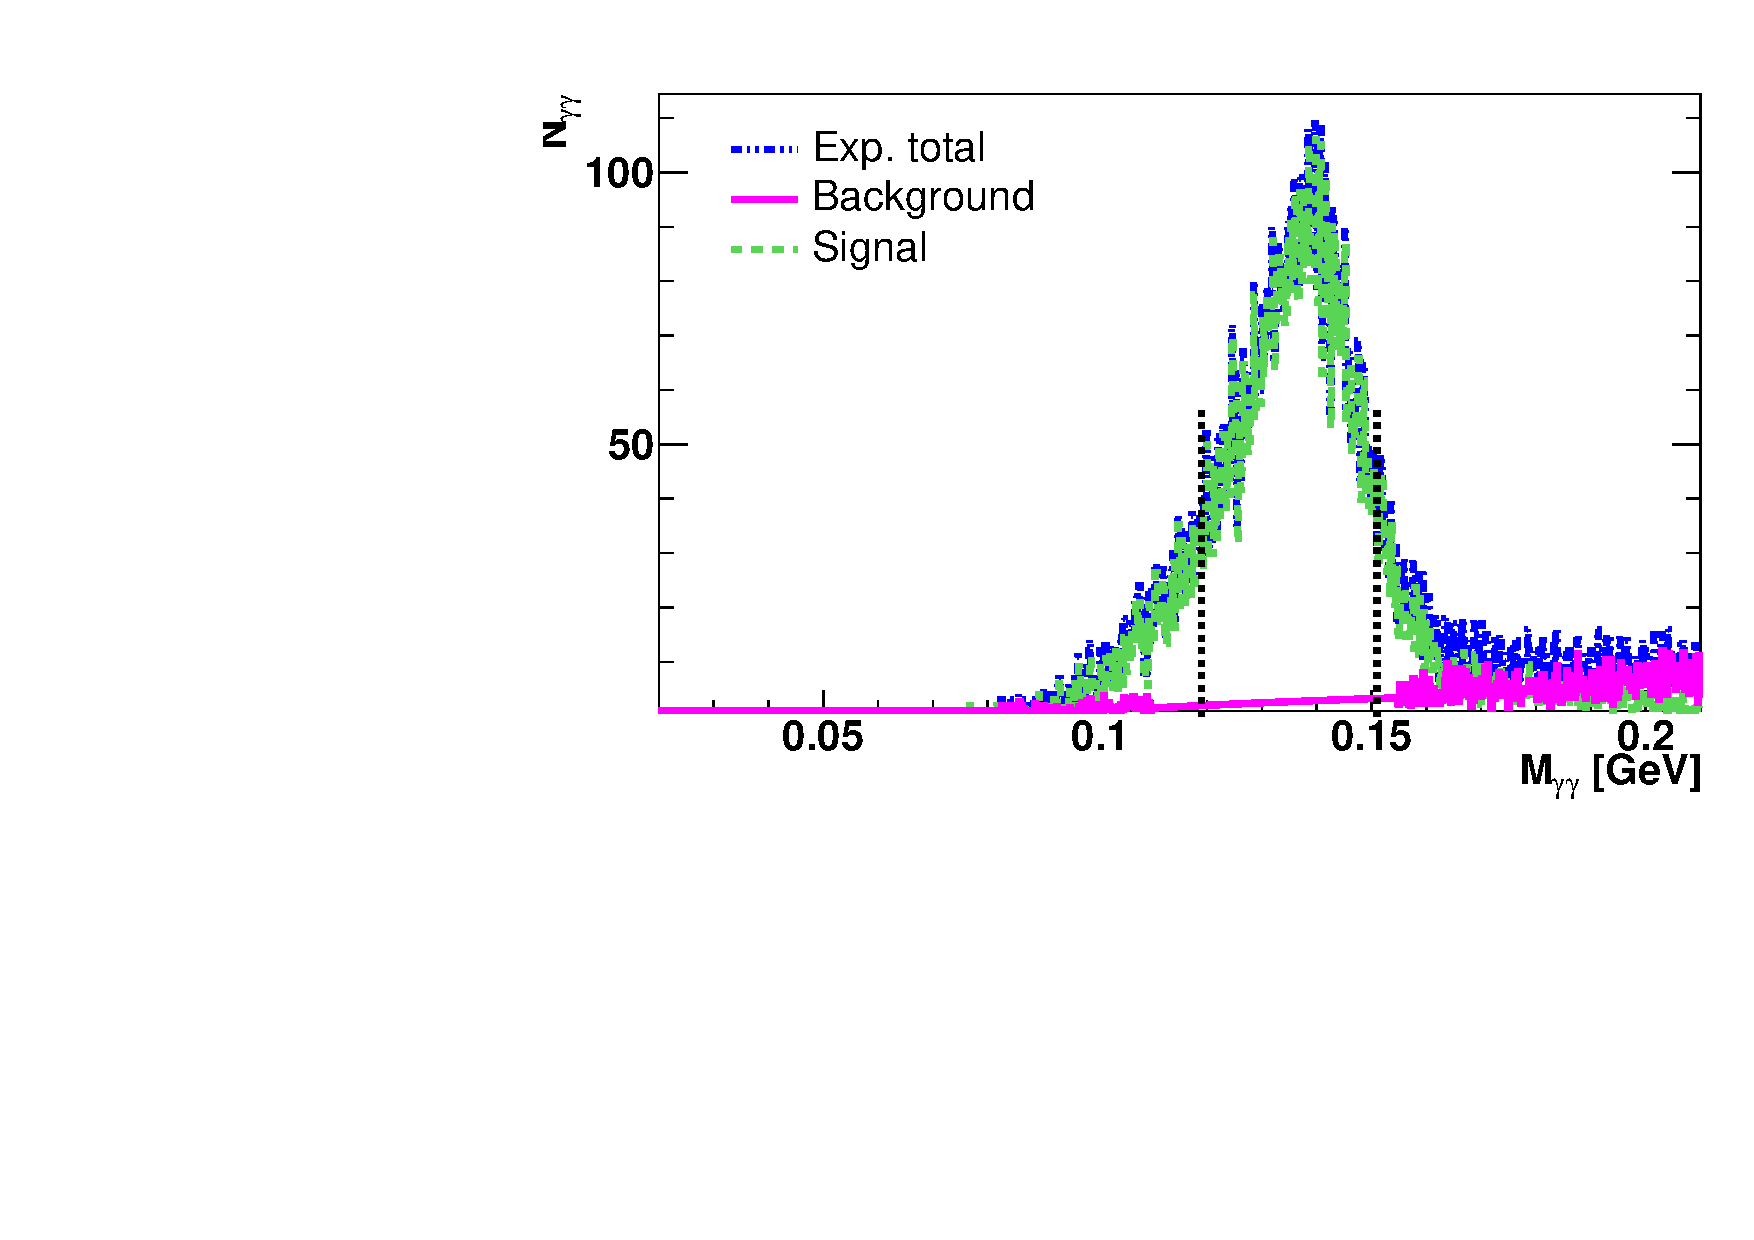
\includegraphics[width=.48\textwidth,natwidth=600,natheight=400]{figure_dataselection/pi0_fit_Z_6.pdf}}
\label{fig:pi0zfit2}
\caption{}
\end{figure}

\begin{figure}[H]
 \ContinuedFloat 
  \centering
  \subfigure[$P_t$ bin 1, $0<p_t<0.15$]{\label{fig:pi0fitpt0}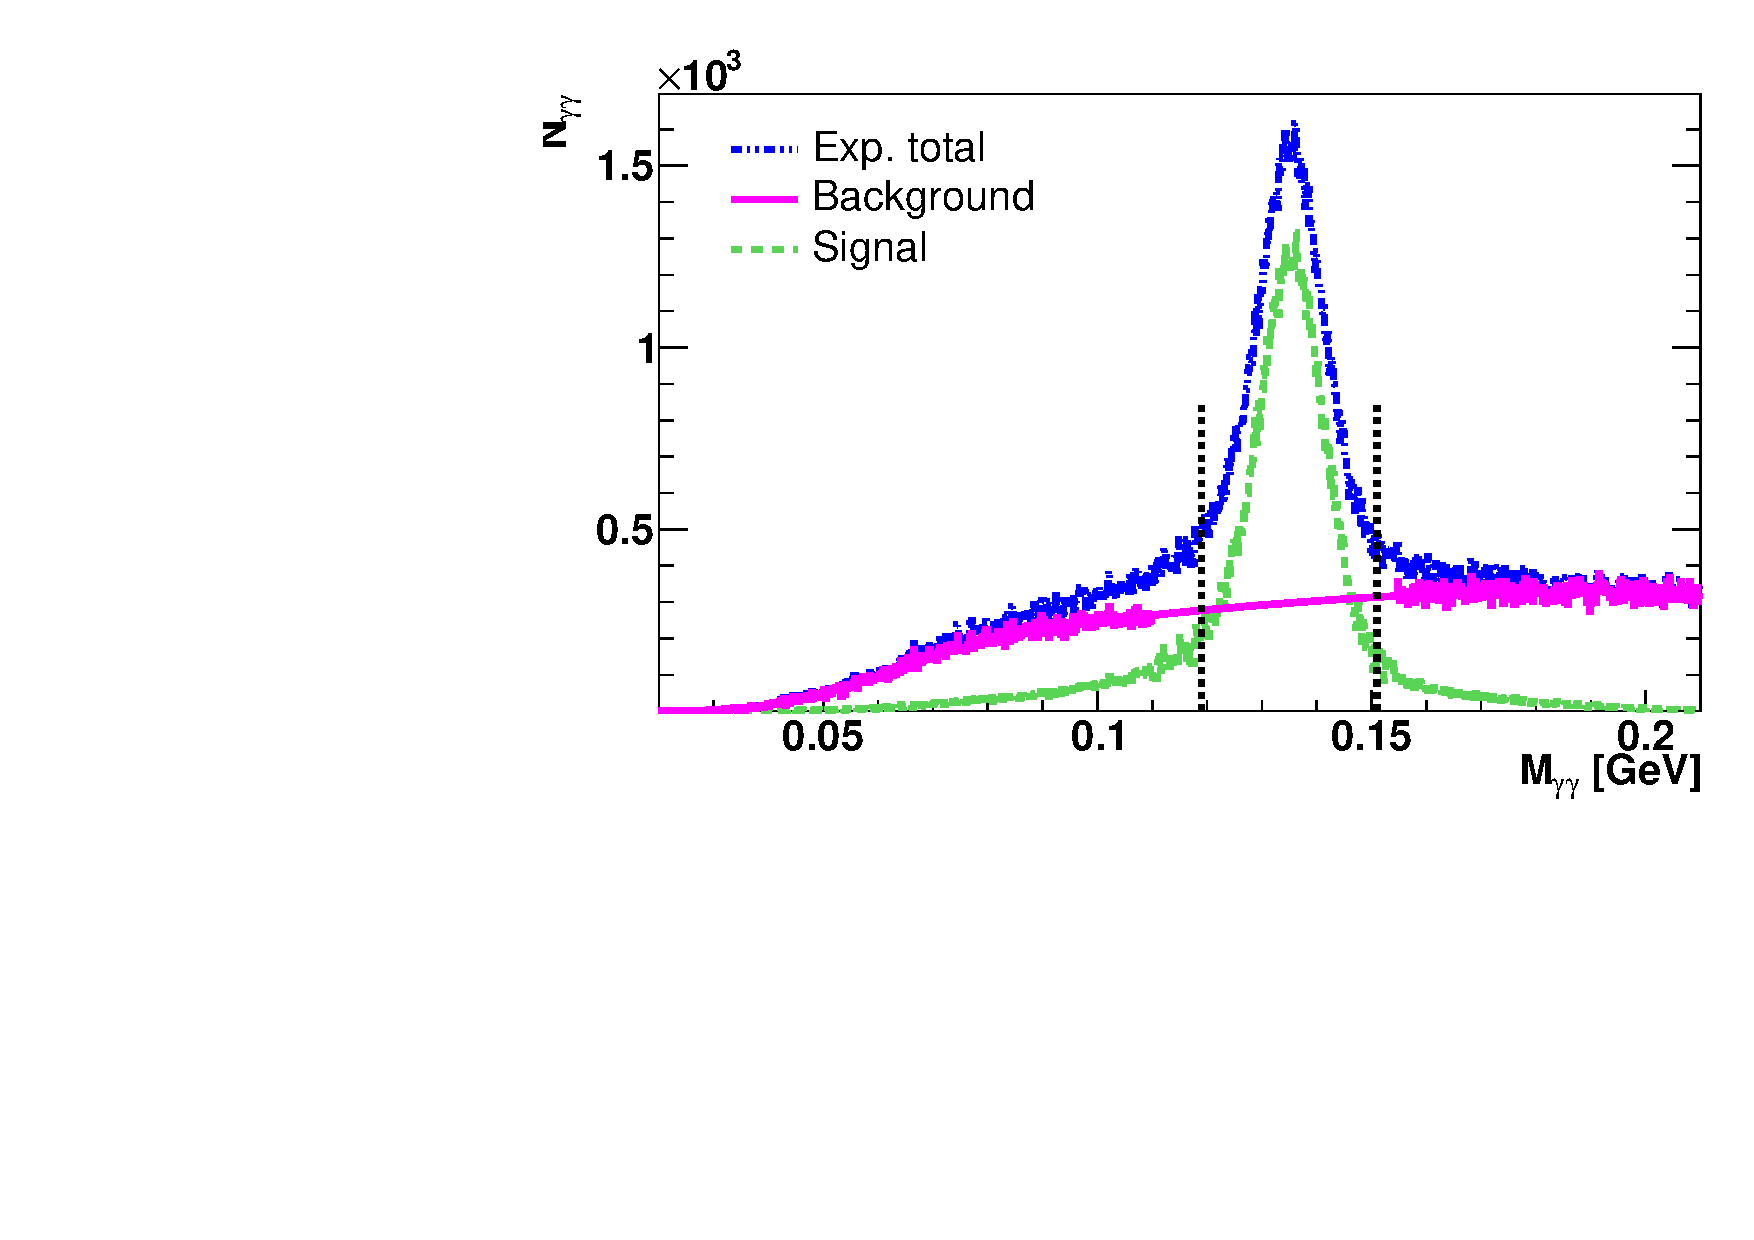
\includegraphics[width=.48\textwidth,natwidth=600,natheight=400]{figure_dataselection/pi0_fit_Pt_0.pdf}}
  \subfigure[$P_t$ bin 2, $0.15<p_t<0.3$]{\label{fig:pi0fitpt1}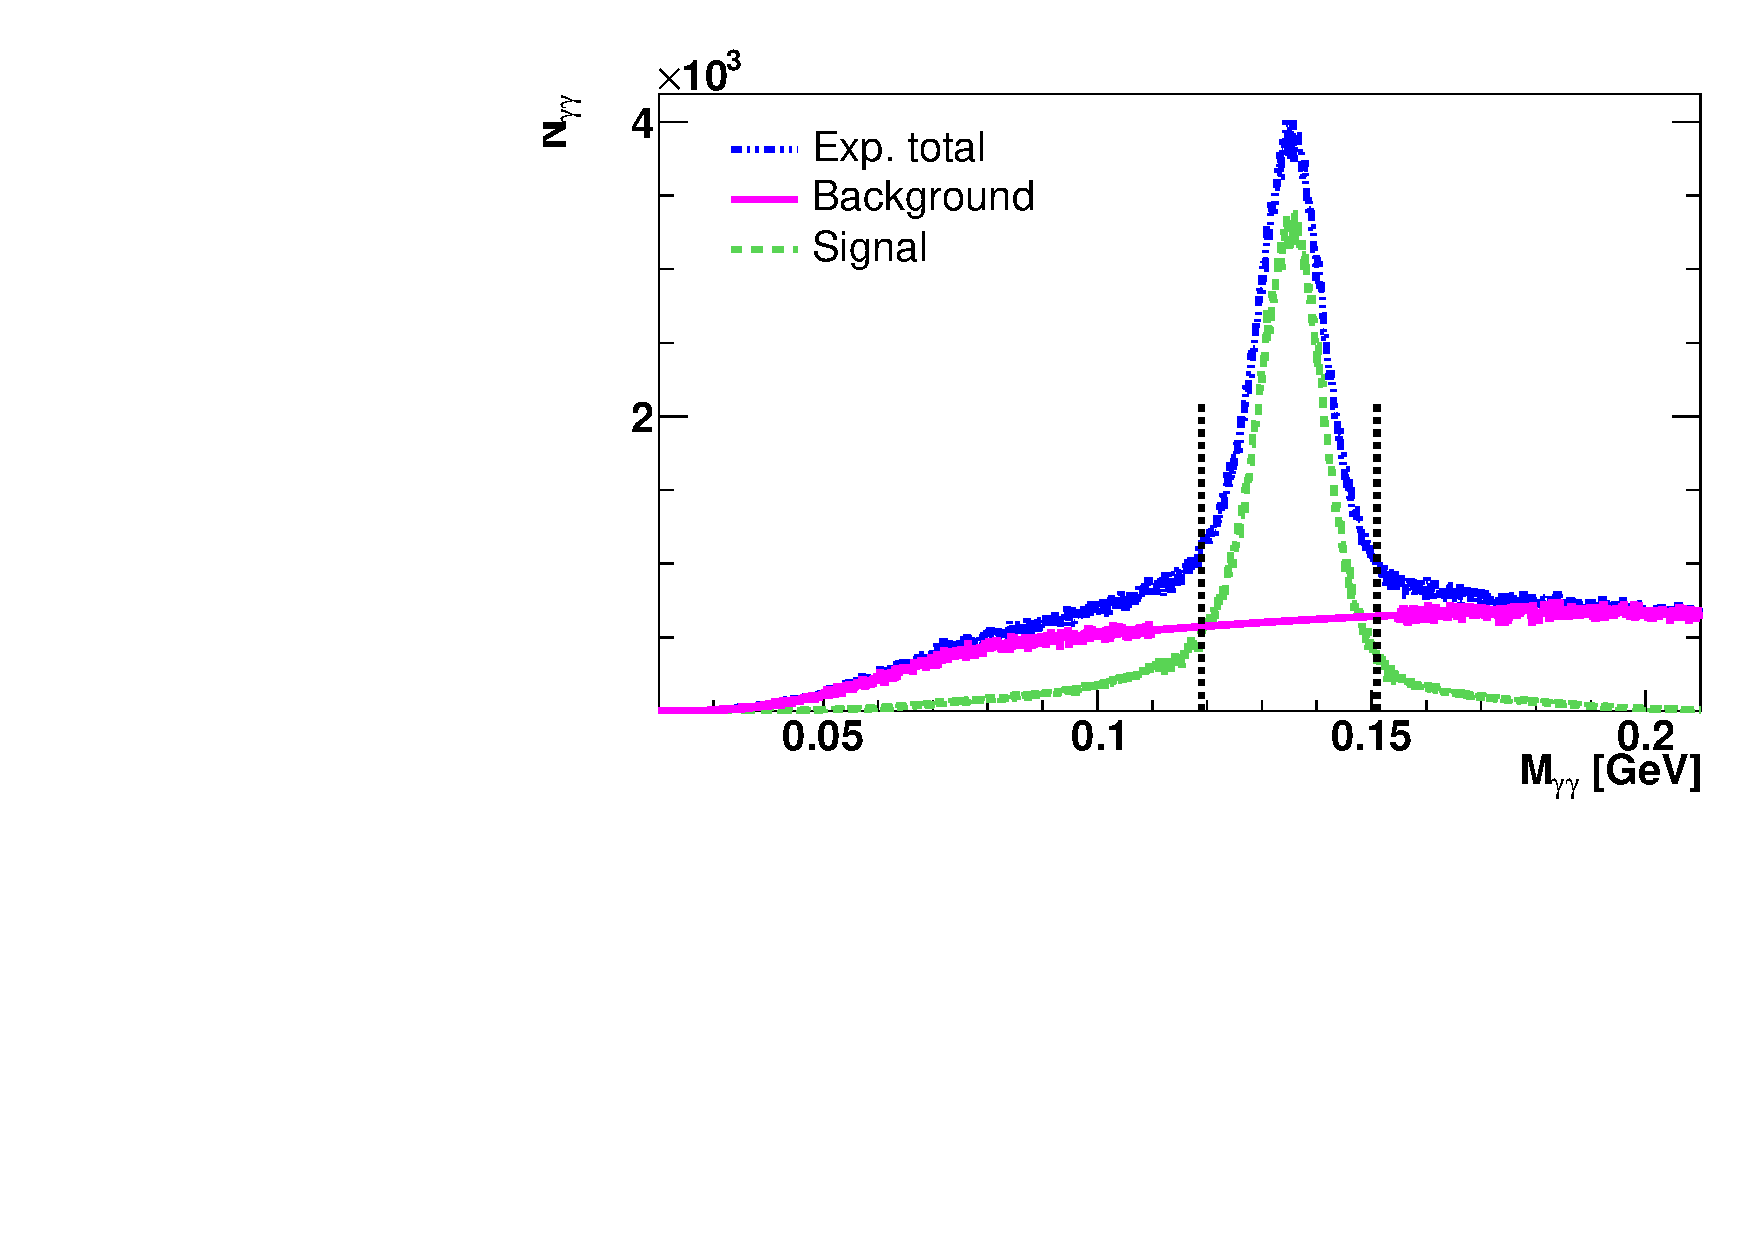
\includegraphics[width=.48\textwidth,natwidth=600,natheight=400]{figure_dataselection/pi0_fit_Pt_1.pdf}}
  \subfigure[$P_t$ bin 3, $0.3<p_t<0.5$]{\label{fig:pi0fitpt2}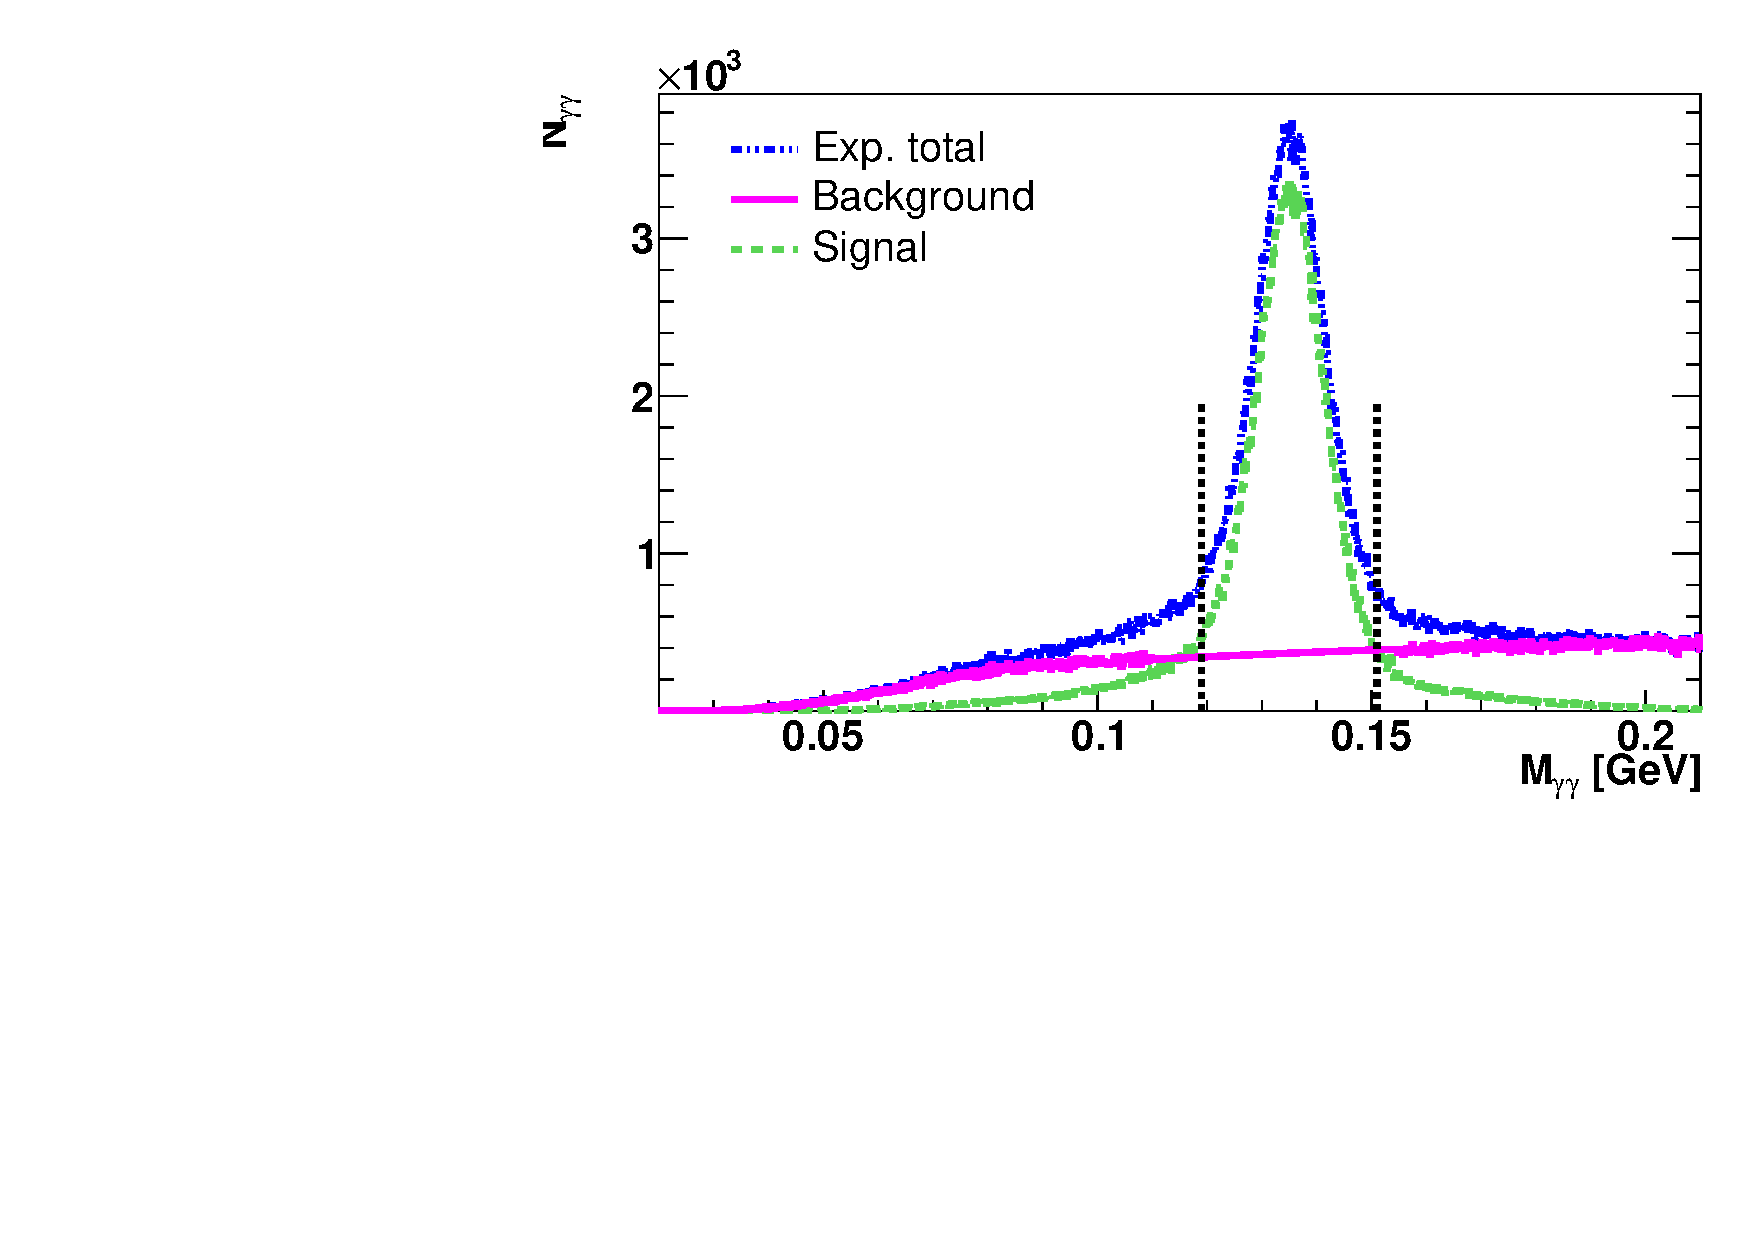
\includegraphics[width=.48\textwidth,natwidth=600,natheight=400]{figure_dataselection/pi0_fit_Pt_2.pdf}}
  \subfigure[$P_t$ bin 4, $0.5<p_t<3$]{\label{fig:pi0fitpt3}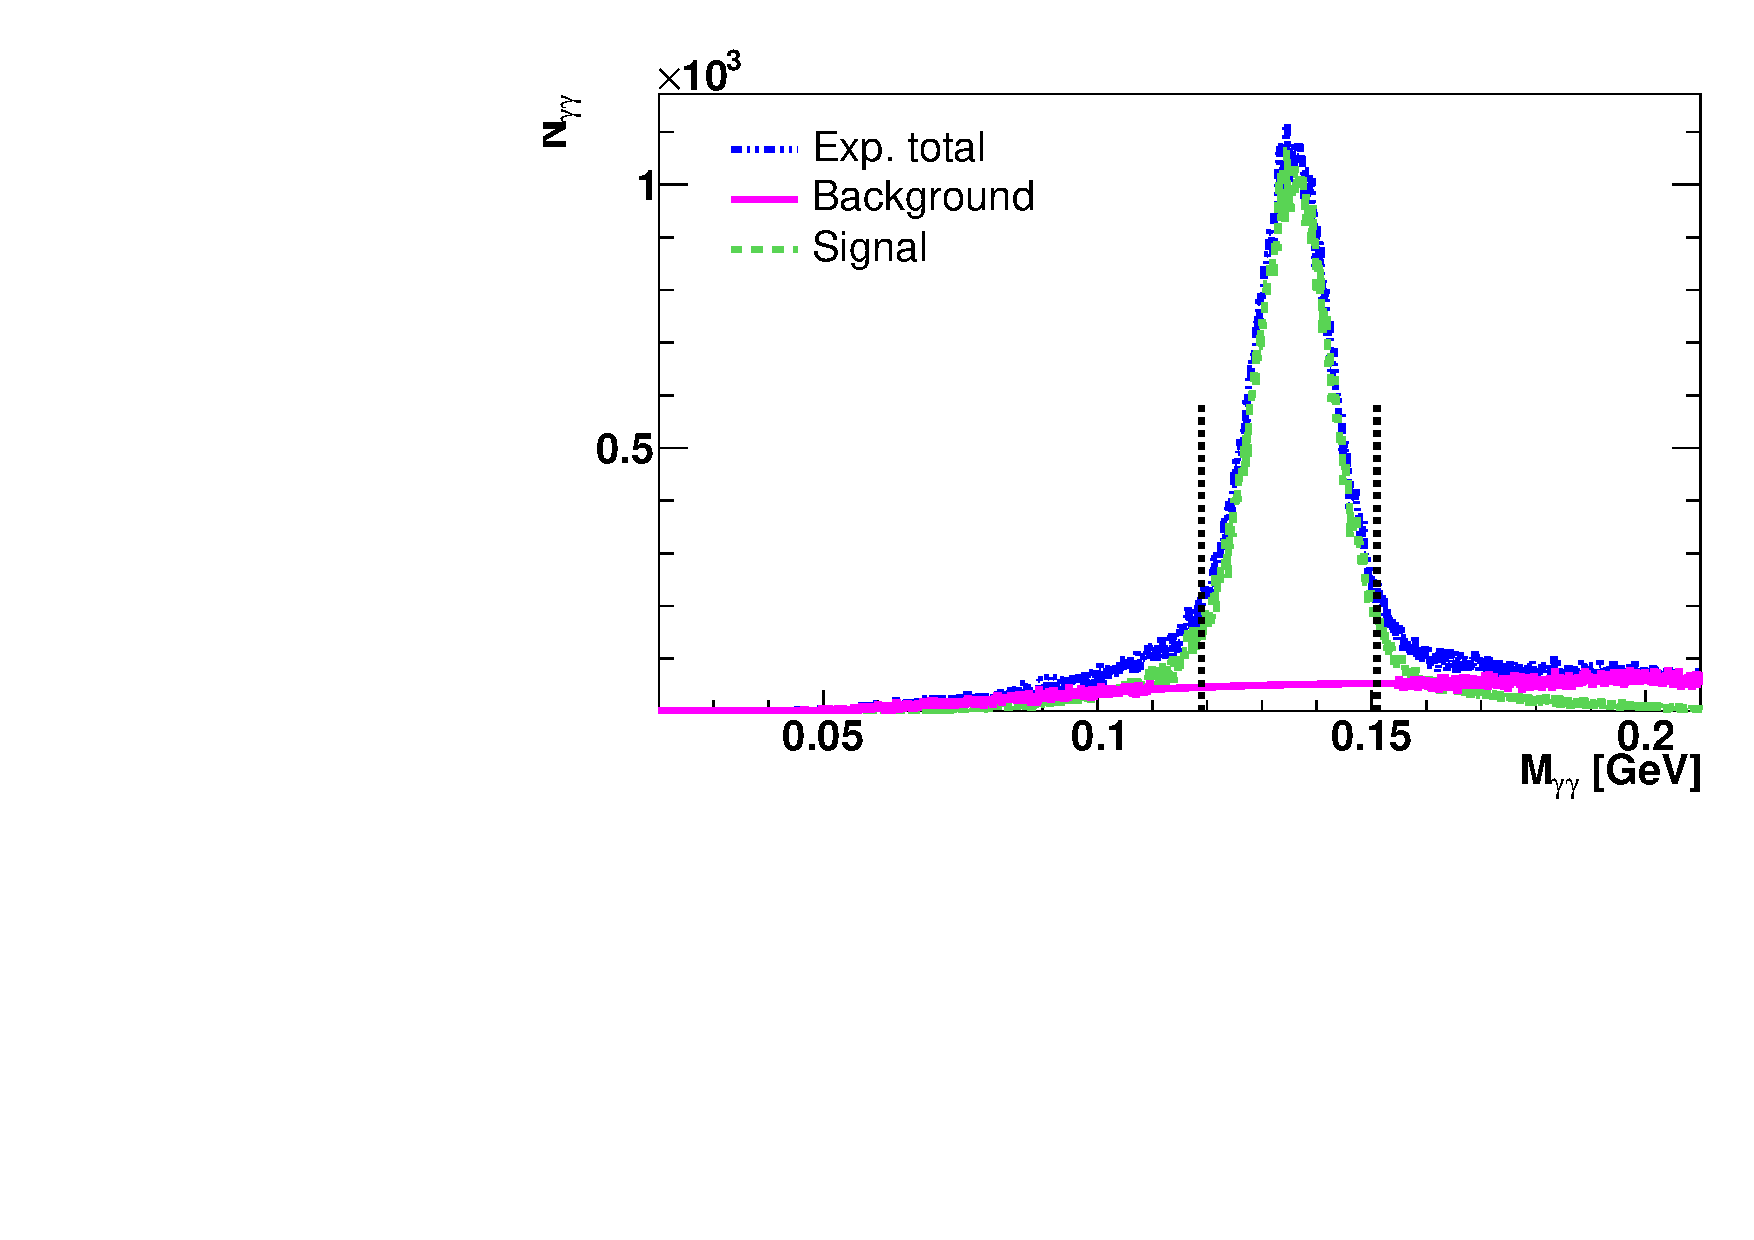
\includegraphics[width=.48\textwidth,natwidth=600,natheight=400]{figure_dataselection/pi0_fit_Pt_3.pdf}}
  \caption{$\pi^0$ fit results for all kinematic bins. Fit method has described in section~\ref{sec:pi0fitsection}. Red line is the background and green line is the signal.}
  \label{fig:pi0ptfit2}
\end{figure}
\subsubsection{\texorpdfstring{Fit results of $\eta$ for all kinematic bins}{Fit result of eta for all kinematic bins}}
\begin{figure}[H]
  \centering     
 \subfigure[$z$ bin 2, $0.2<z<0.3$]{\label{fig:etafitz7}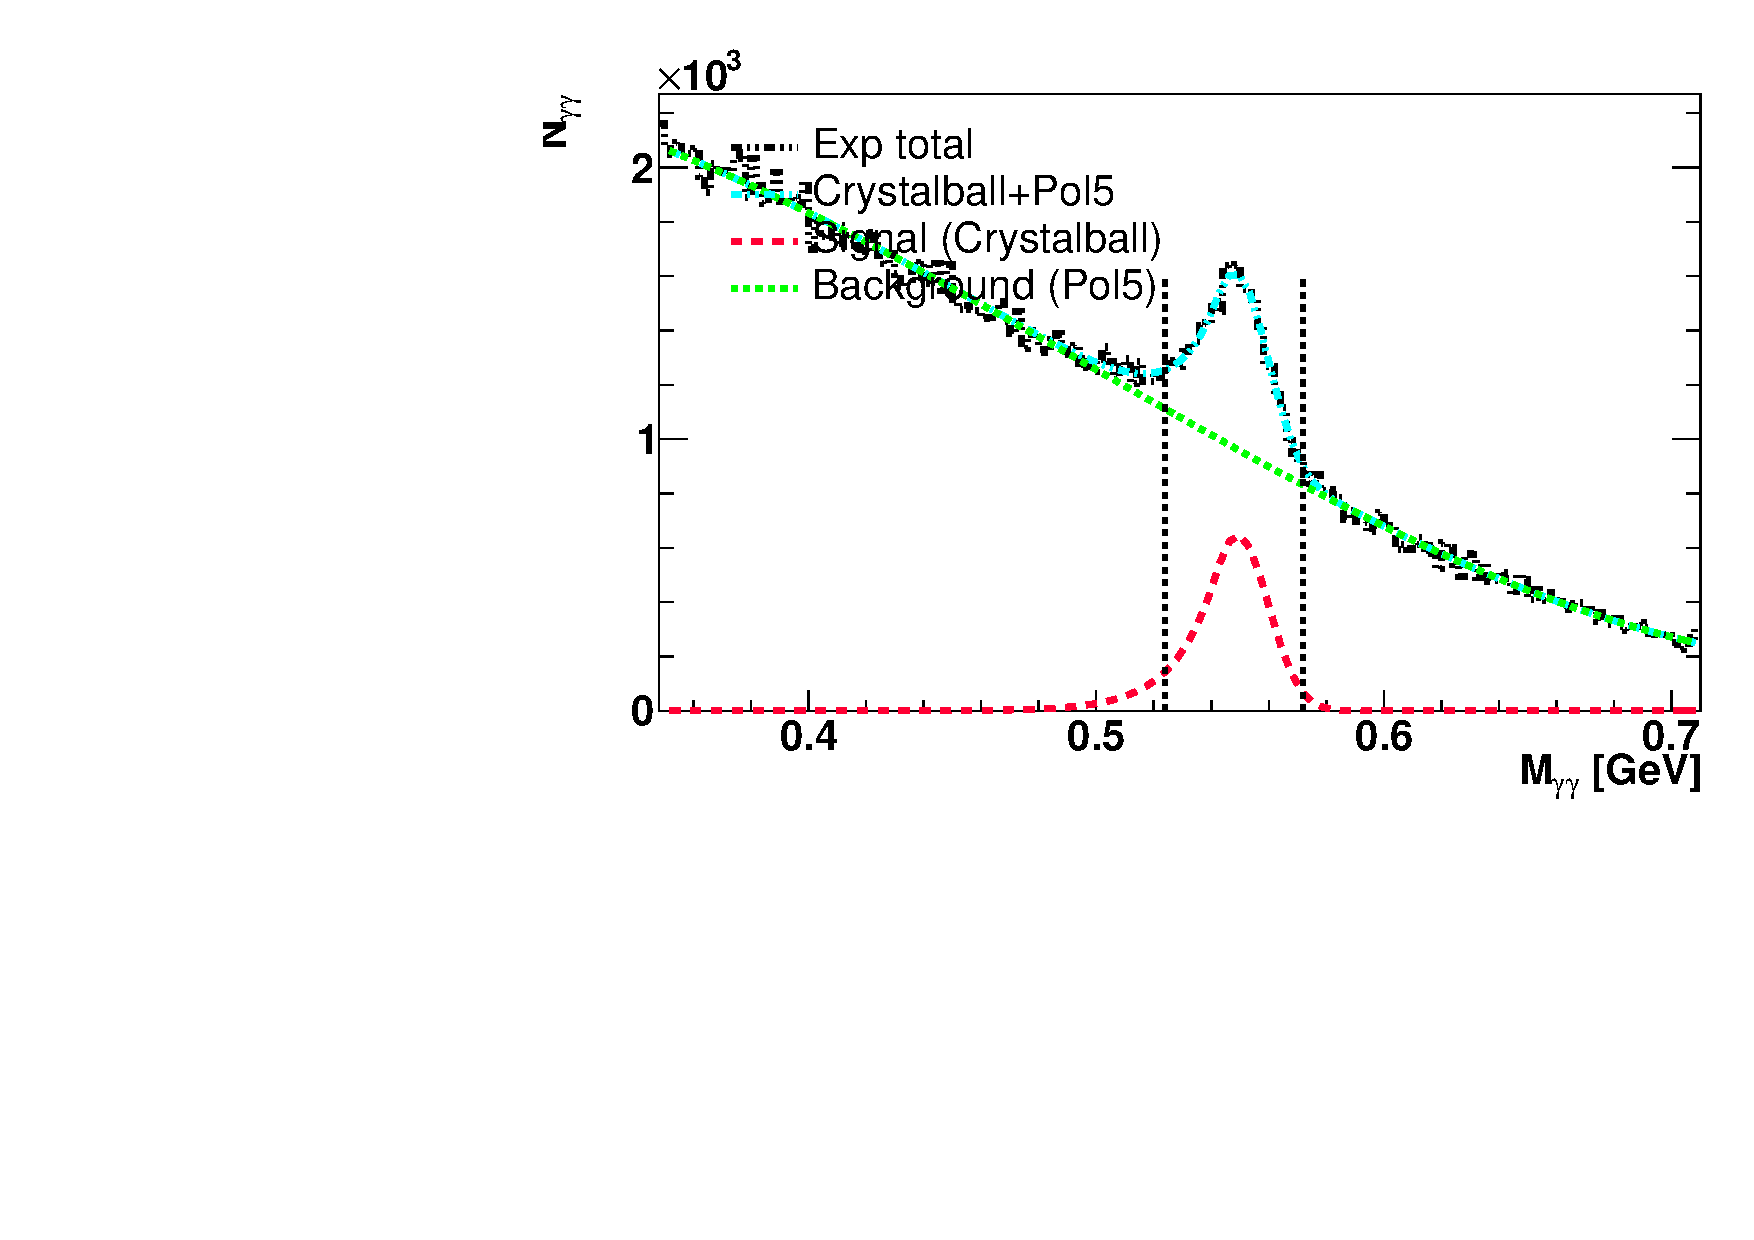
\includegraphics[width=.48\textwidth,natwidth=600,natheight=400]{figure_dataselection/eta_fitall_Z_2.pdf}}
\subfigure[$z$ bin 2, $0.2<z<0.3$]{\label{fig:etafitz42}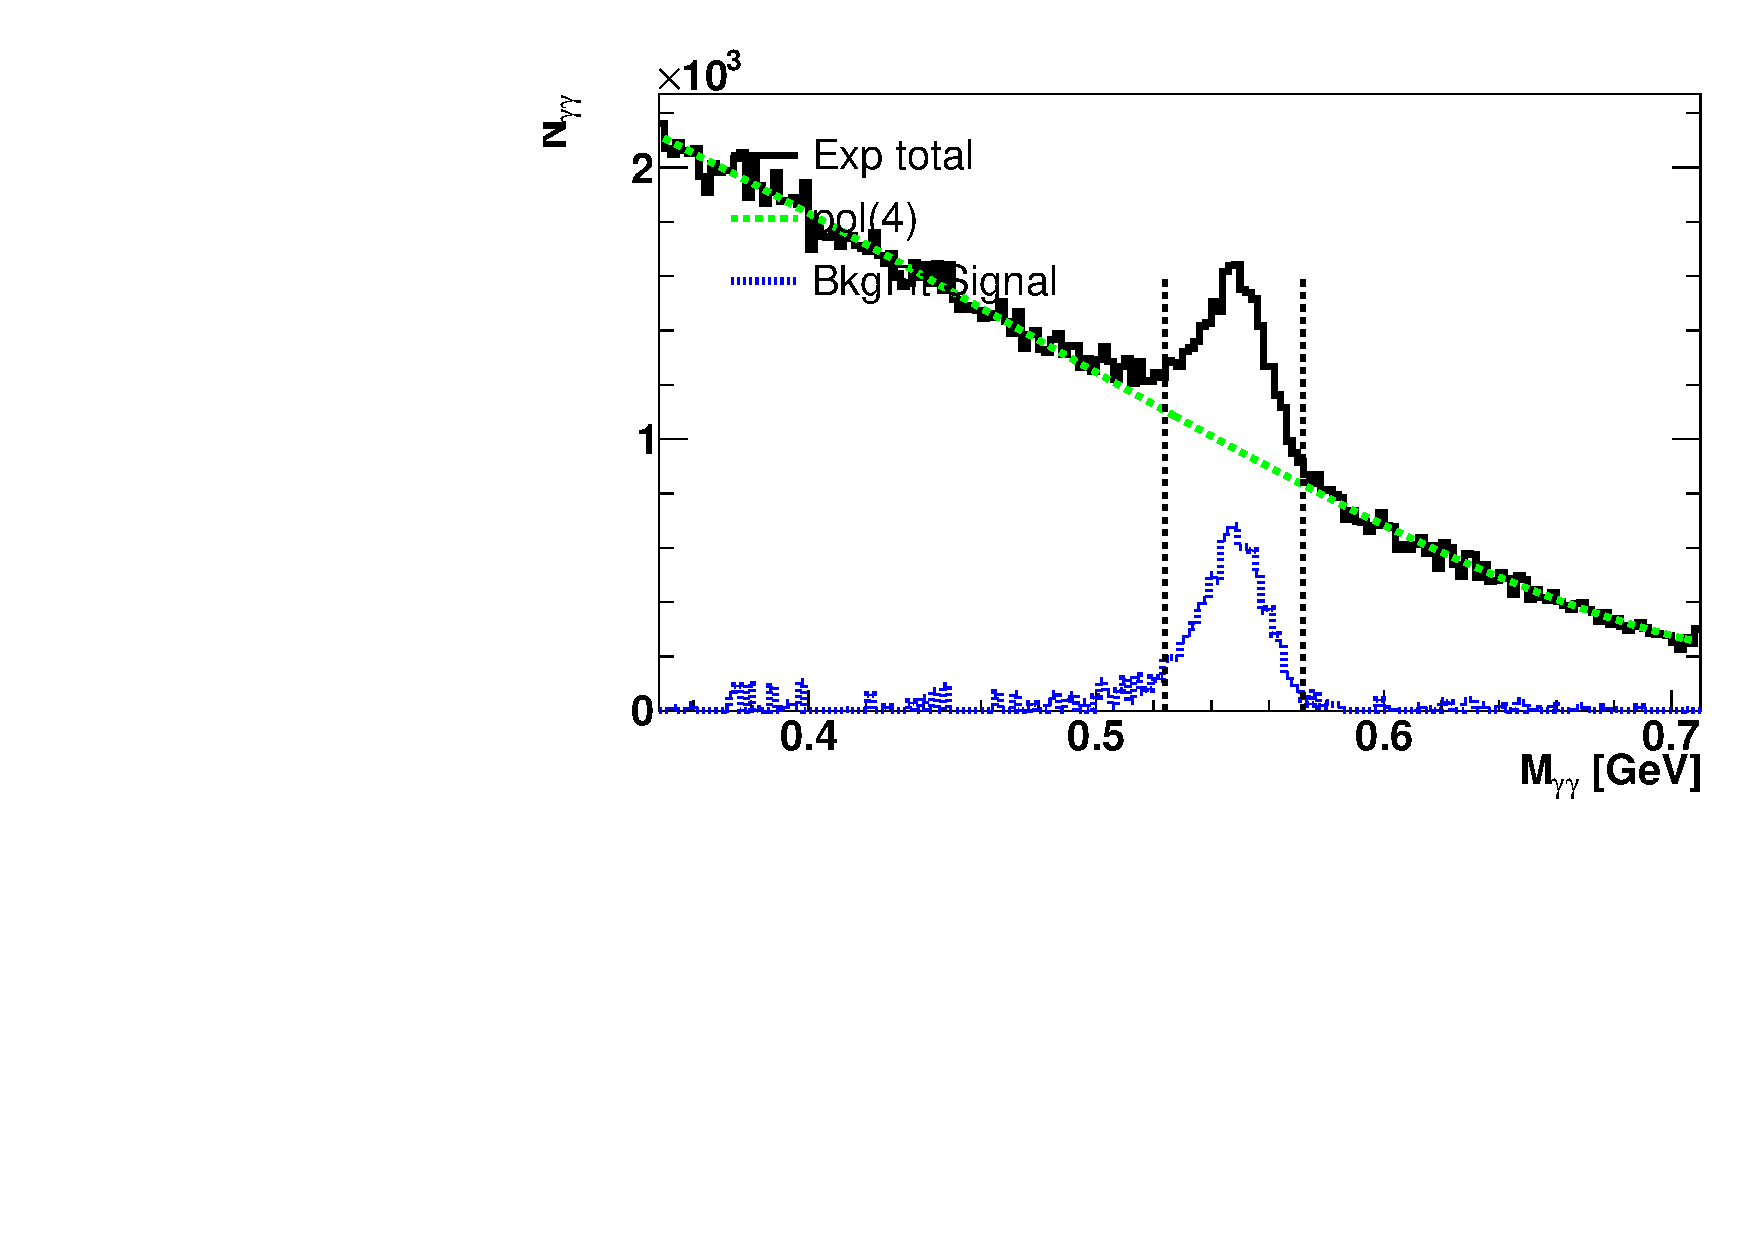
\includegraphics[width=.48\textwidth,natwidth=600,natheight=400]{figure_dataselection/eta_fitbkg_Z_2.pdf}}
  \subfigure[$z$ bin 3, $0.3<z<0.4$]{\label{fig:etafitz7}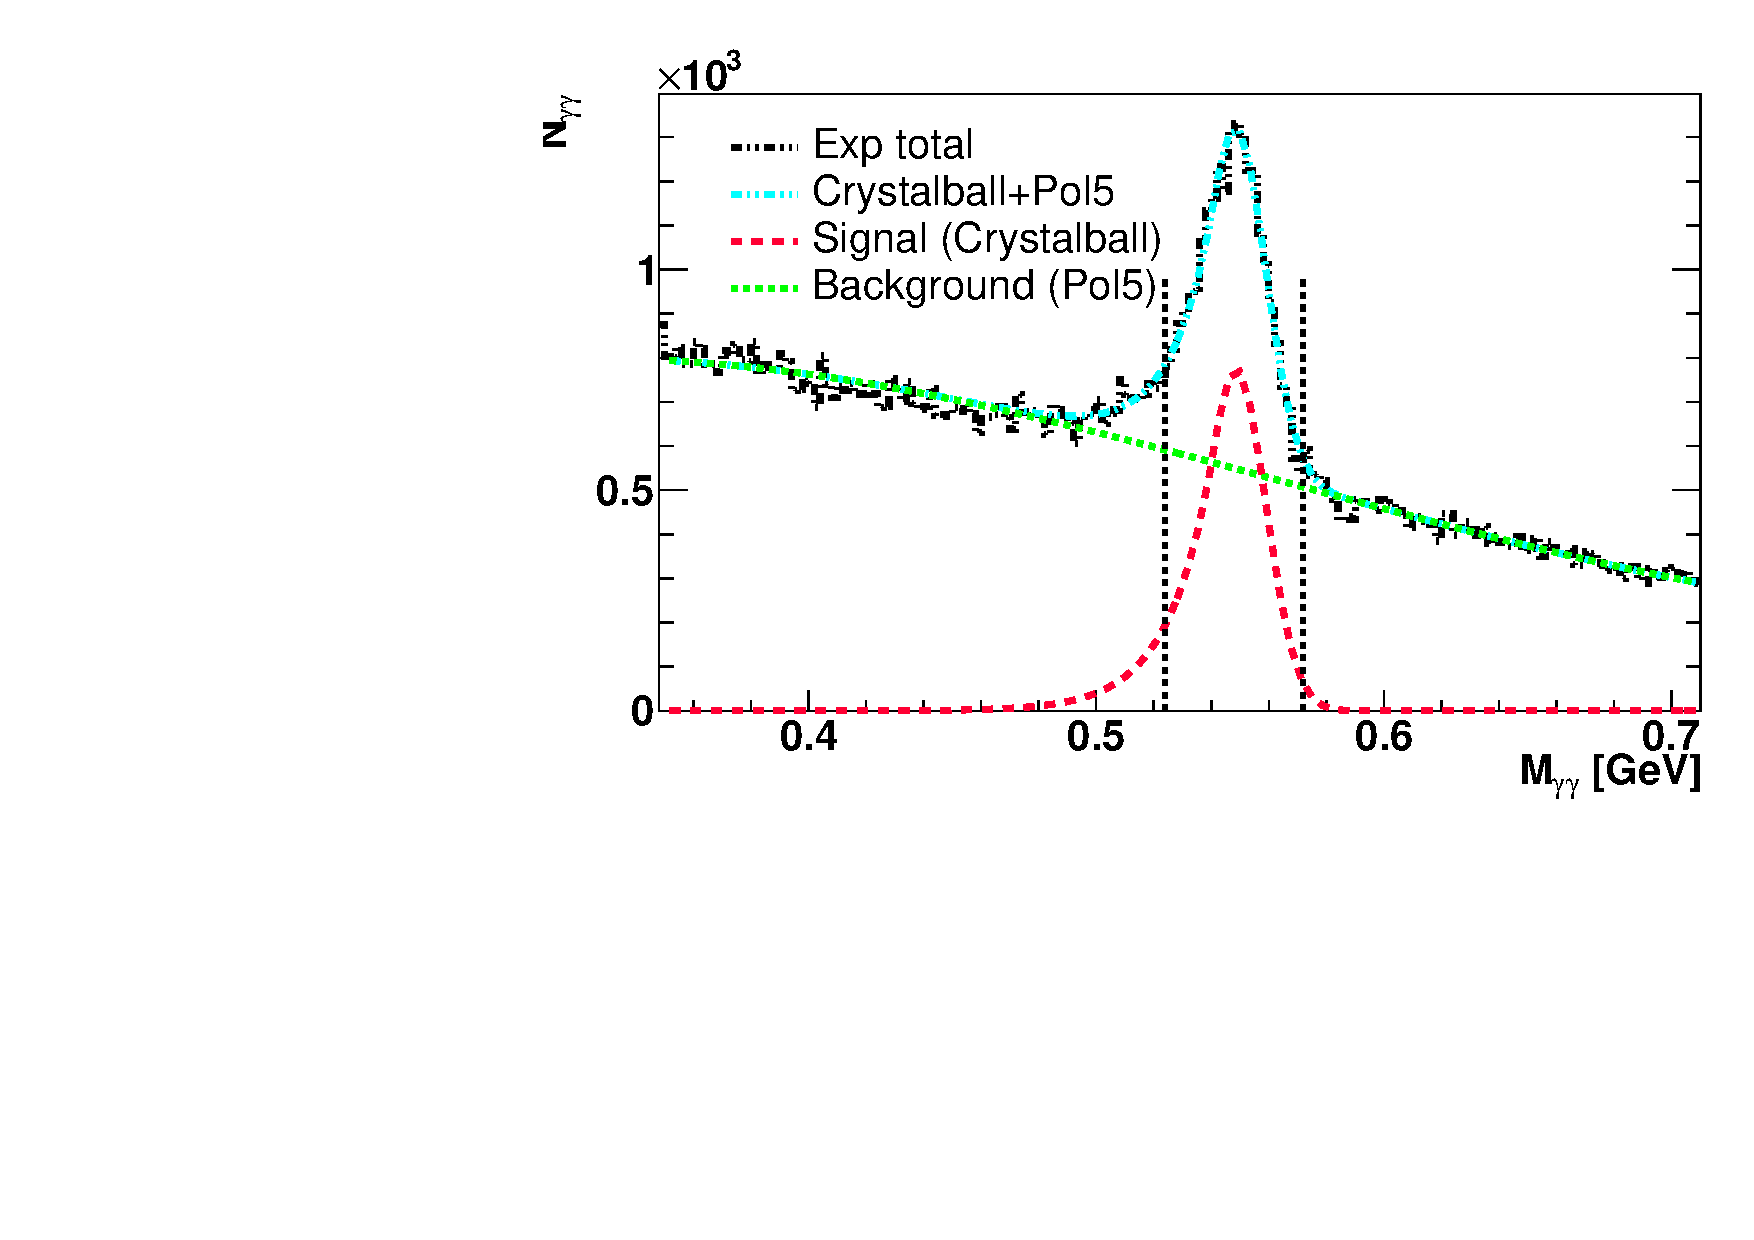
\includegraphics[width=.48\textwidth,natwidth=600,natheight=400]{figure_dataselection/eta_fitall_Z_3.pdf}}
\subfigure[$z$ bin 3, $0.3<z<0.4$]{\label{fig:etafitz42}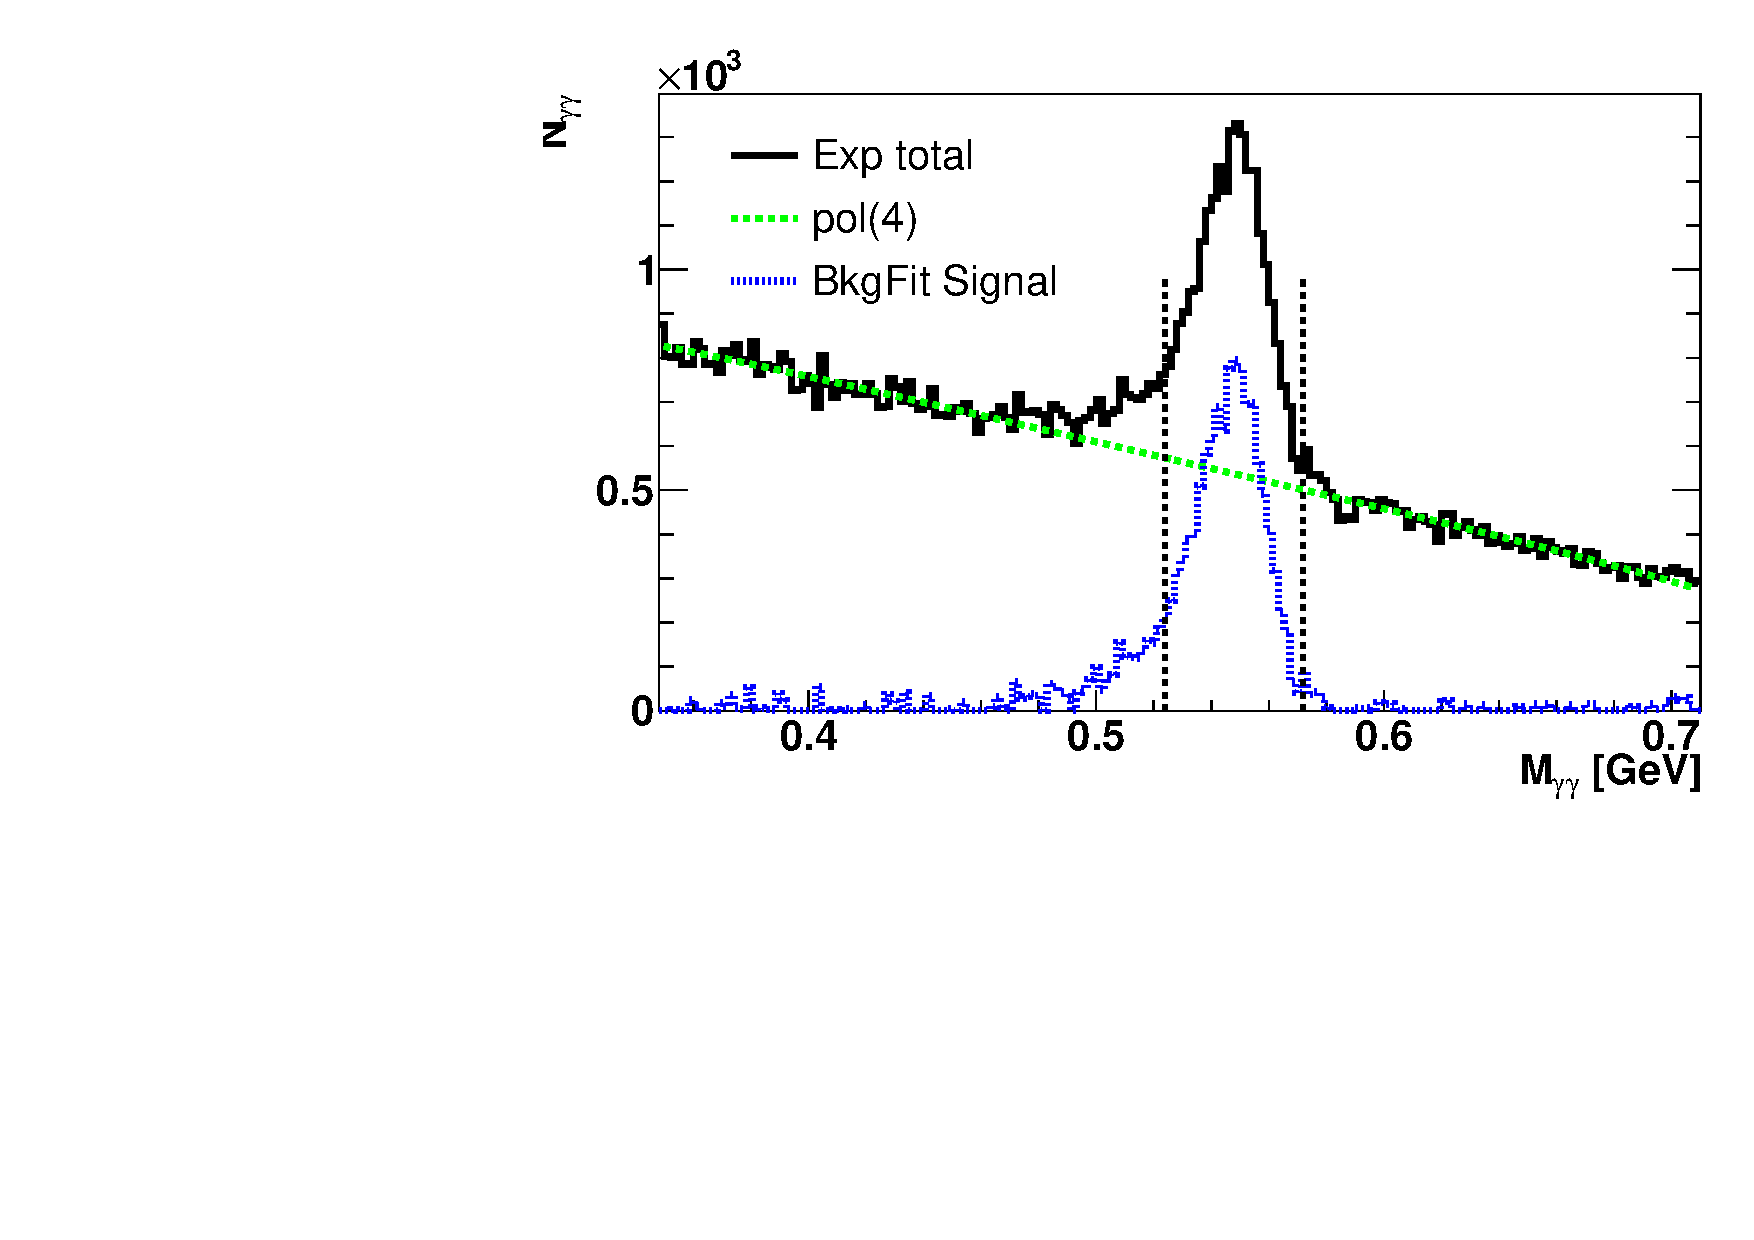
\includegraphics[width=.48\textwidth,natwidth=600,natheight=400]{figure_dataselection/eta_fitbkg_Z_3.pdf}}
  \subfigure[$z$ bin 4, $0.4<z<0.5$]{\label{fig:etafitz4}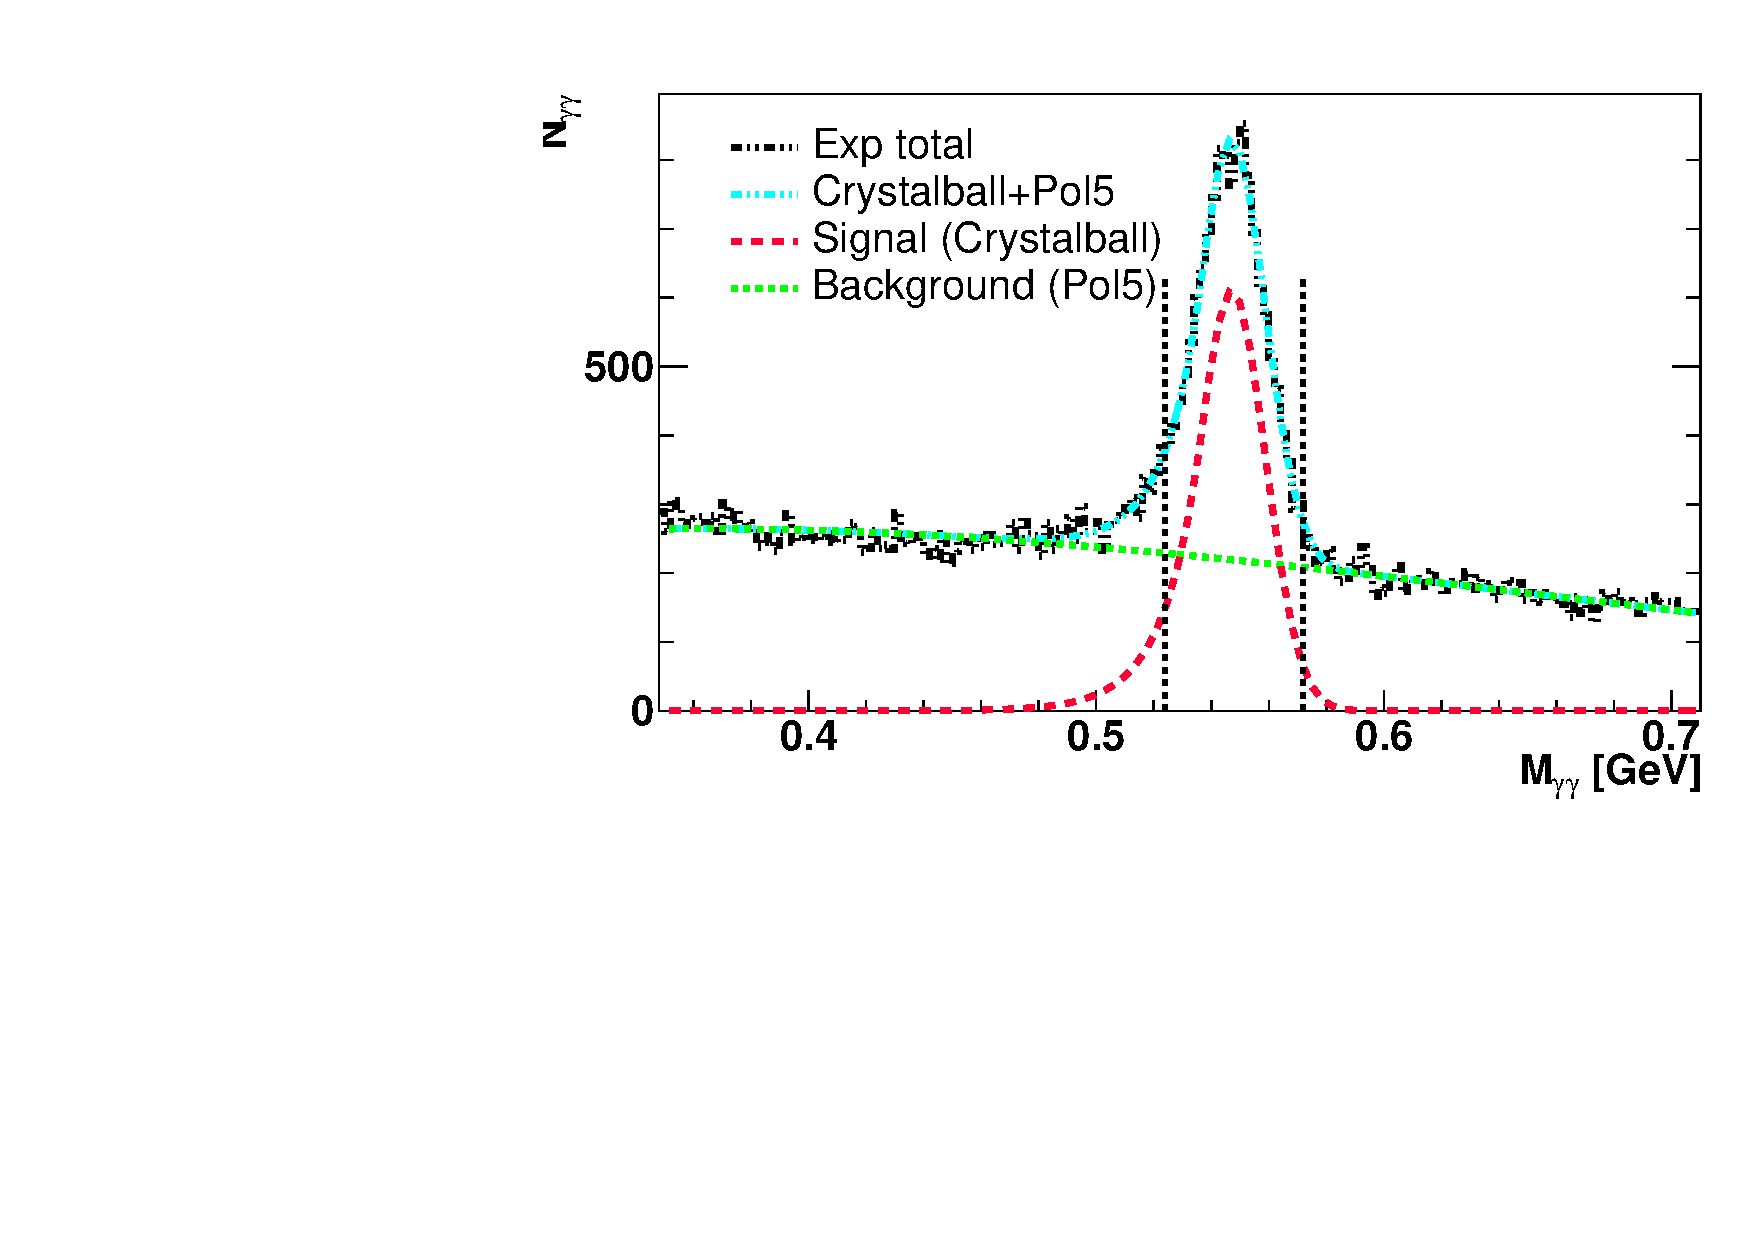
\includegraphics[width=.48\textwidth,natwidth=600,natheight=400]{figure_dataselection/eta_fitall_Z_4.pdf}}
\subfigure[$z$ bin 4, $0.4<z<0.5$]{\label{fig:etafitz42}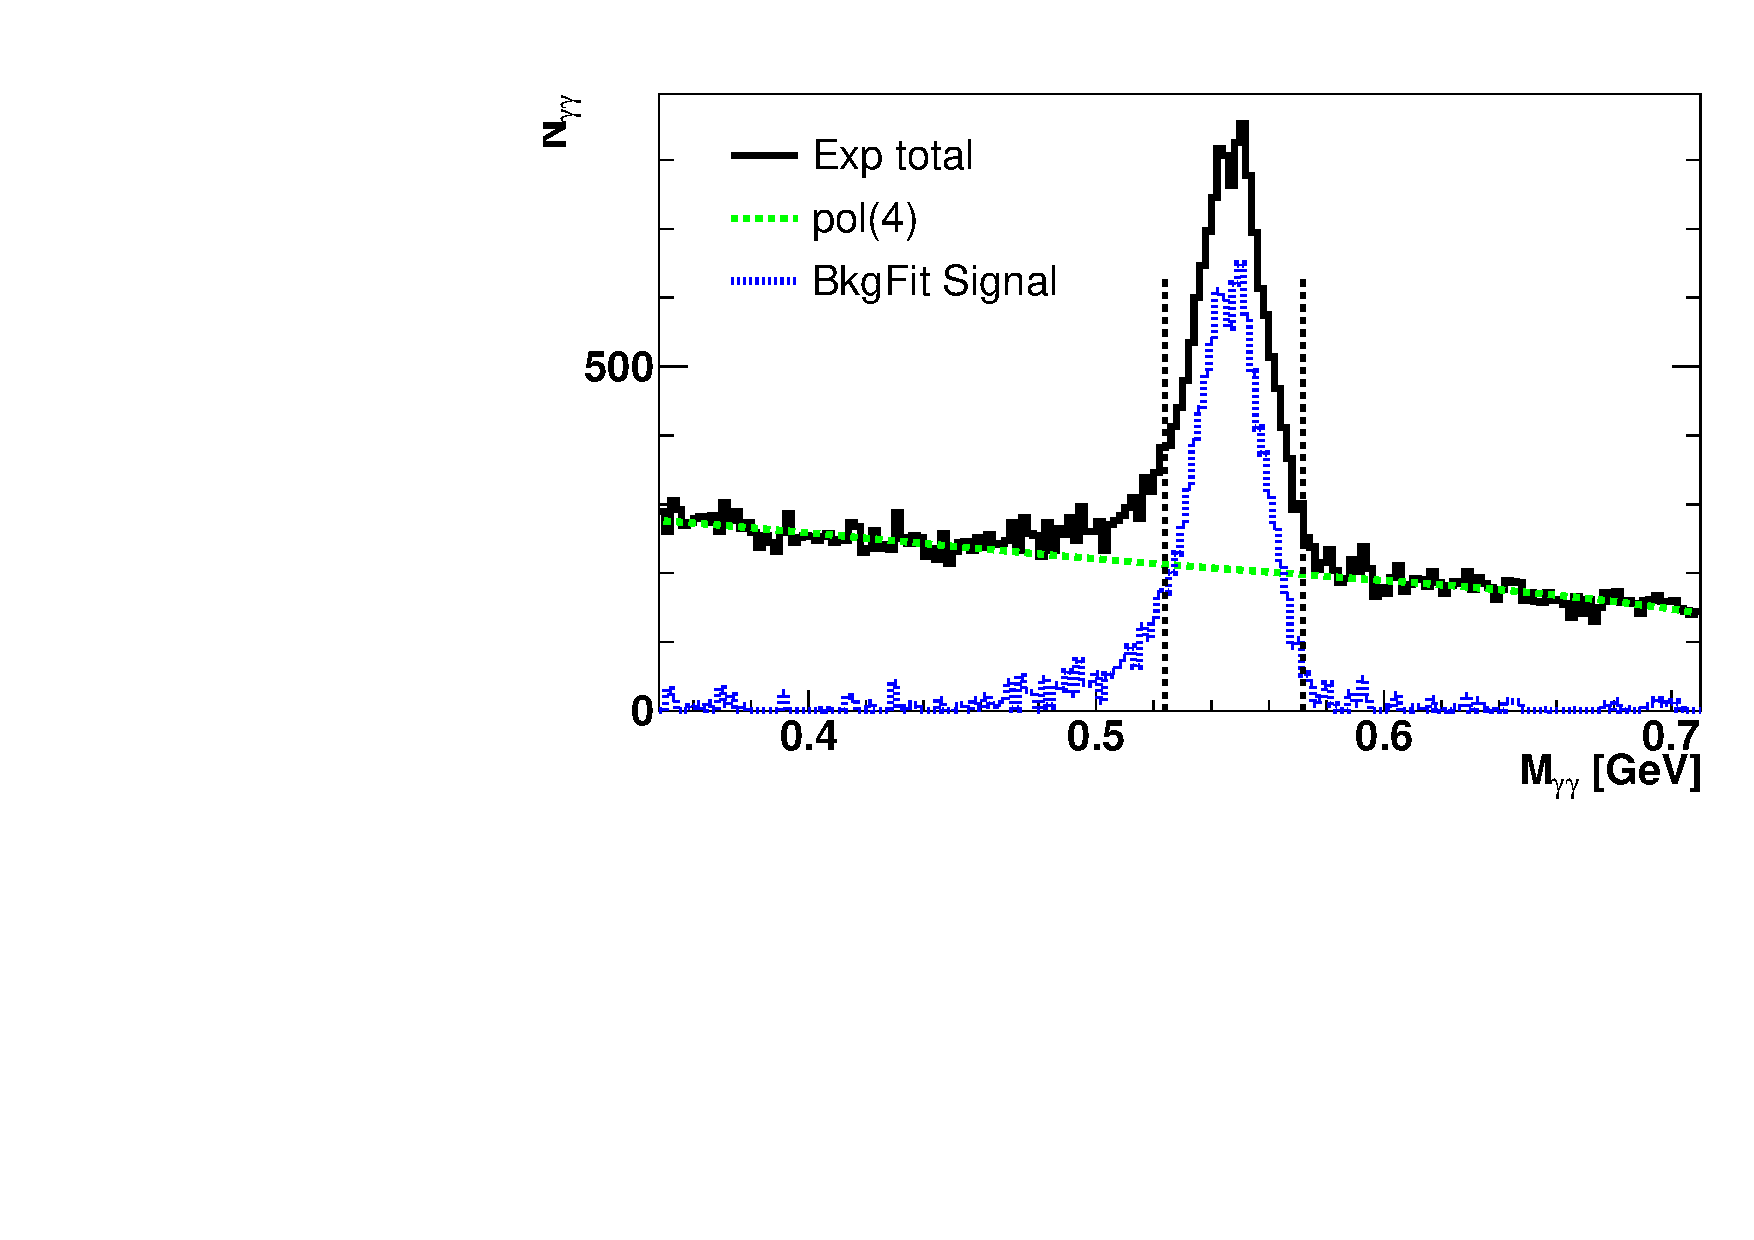
\includegraphics[width=.48\textwidth,natwidth=600,natheight=400]{figure_dataselection/eta_fitbkg_Z_4.pdf}}
\label{fig:etazfit}
\caption{}
\end{figure}
\begin{figure}[H]
  \centering 
  \subfigure[$z$ bin 5, $0.5<z<0.6$]{\label{fig:etafitz5}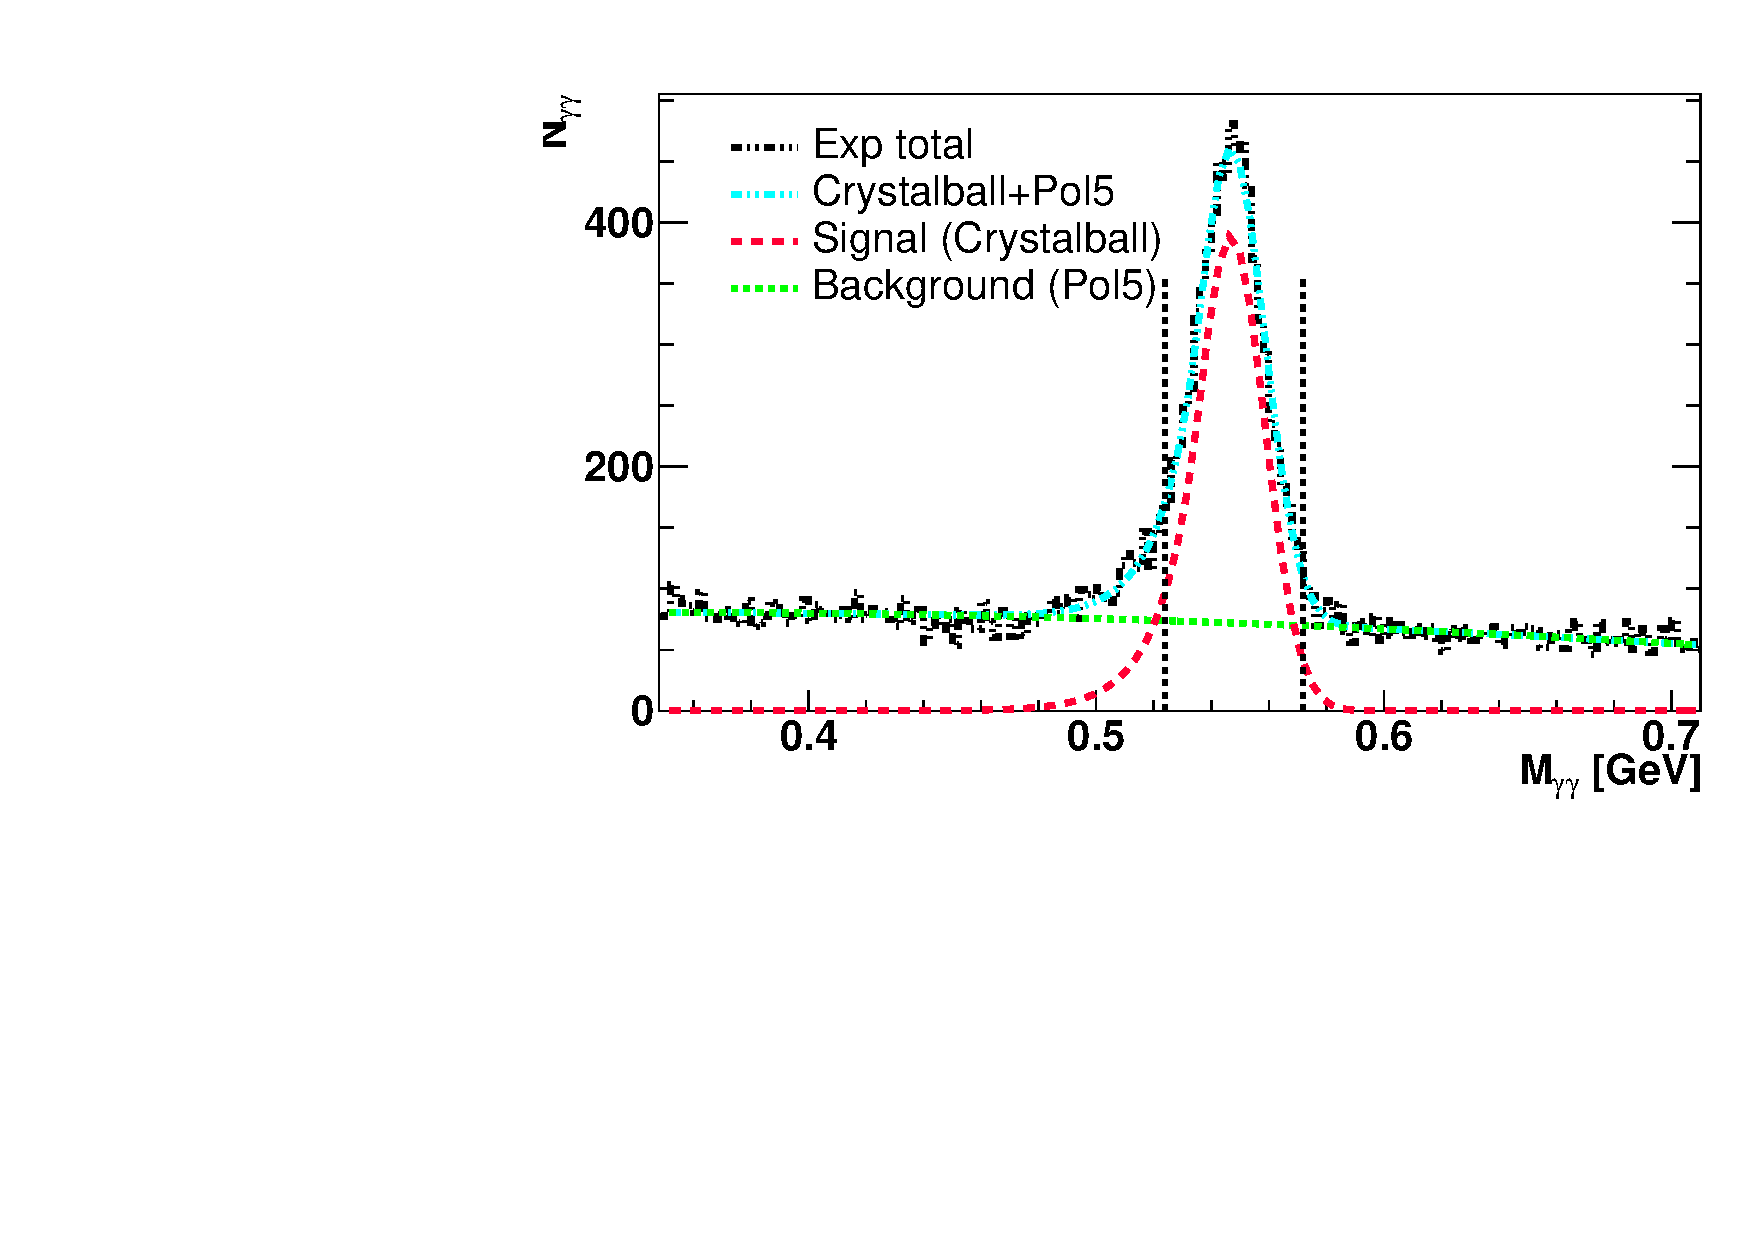
\includegraphics[width=.48\textwidth,natwidth=600,natheight=400]{figure_dataselection/eta_fitall_Z_5.pdf}}
\subfigure[$z$ bin 5, $0.5<z<0.6$]{\label{fig:etafitz52}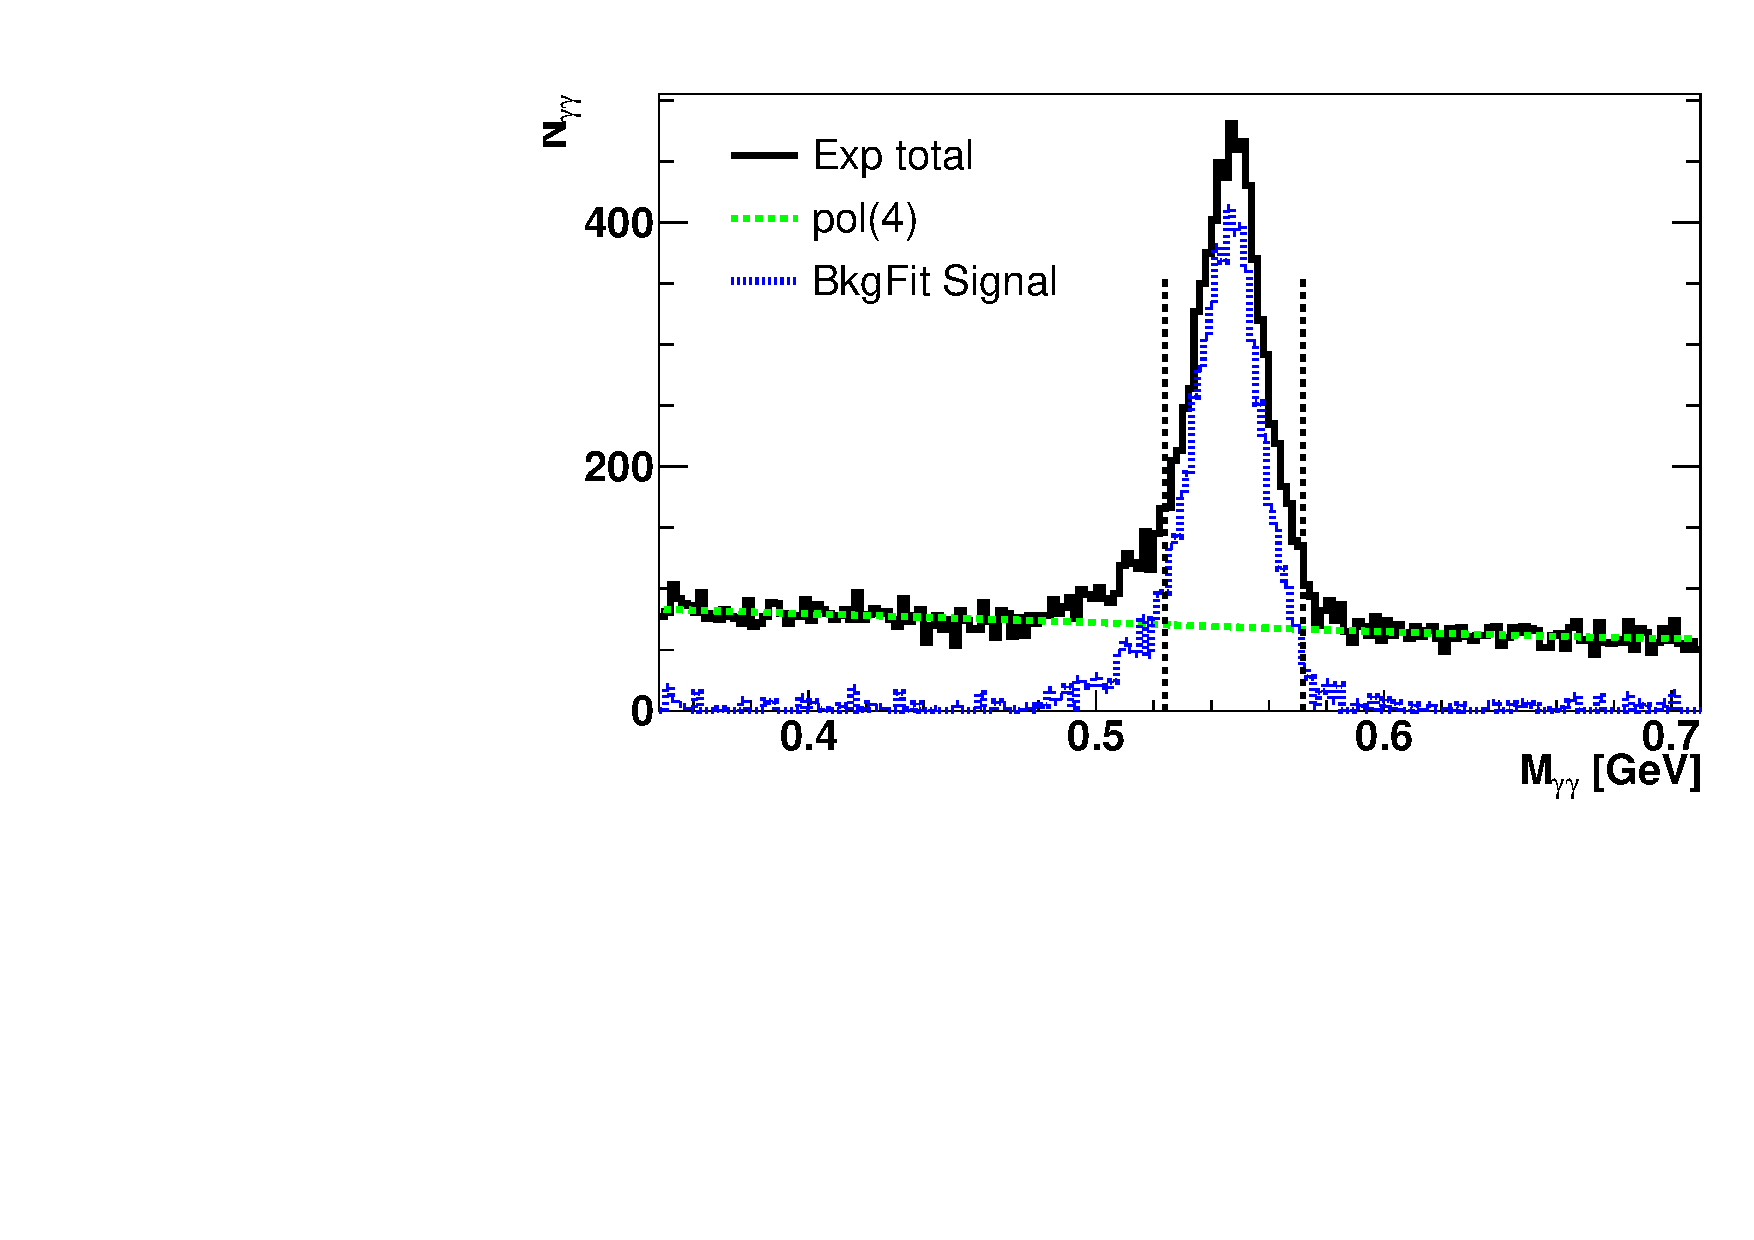
\includegraphics[width=.48\textwidth,natwidth=600,natheight=400]{figure_dataselection/eta_fitbkg_Z_5.pdf}}
  \subfigure[$z$ bin 6, $0.6<z<0.7$]{\label{fig:etafitz6}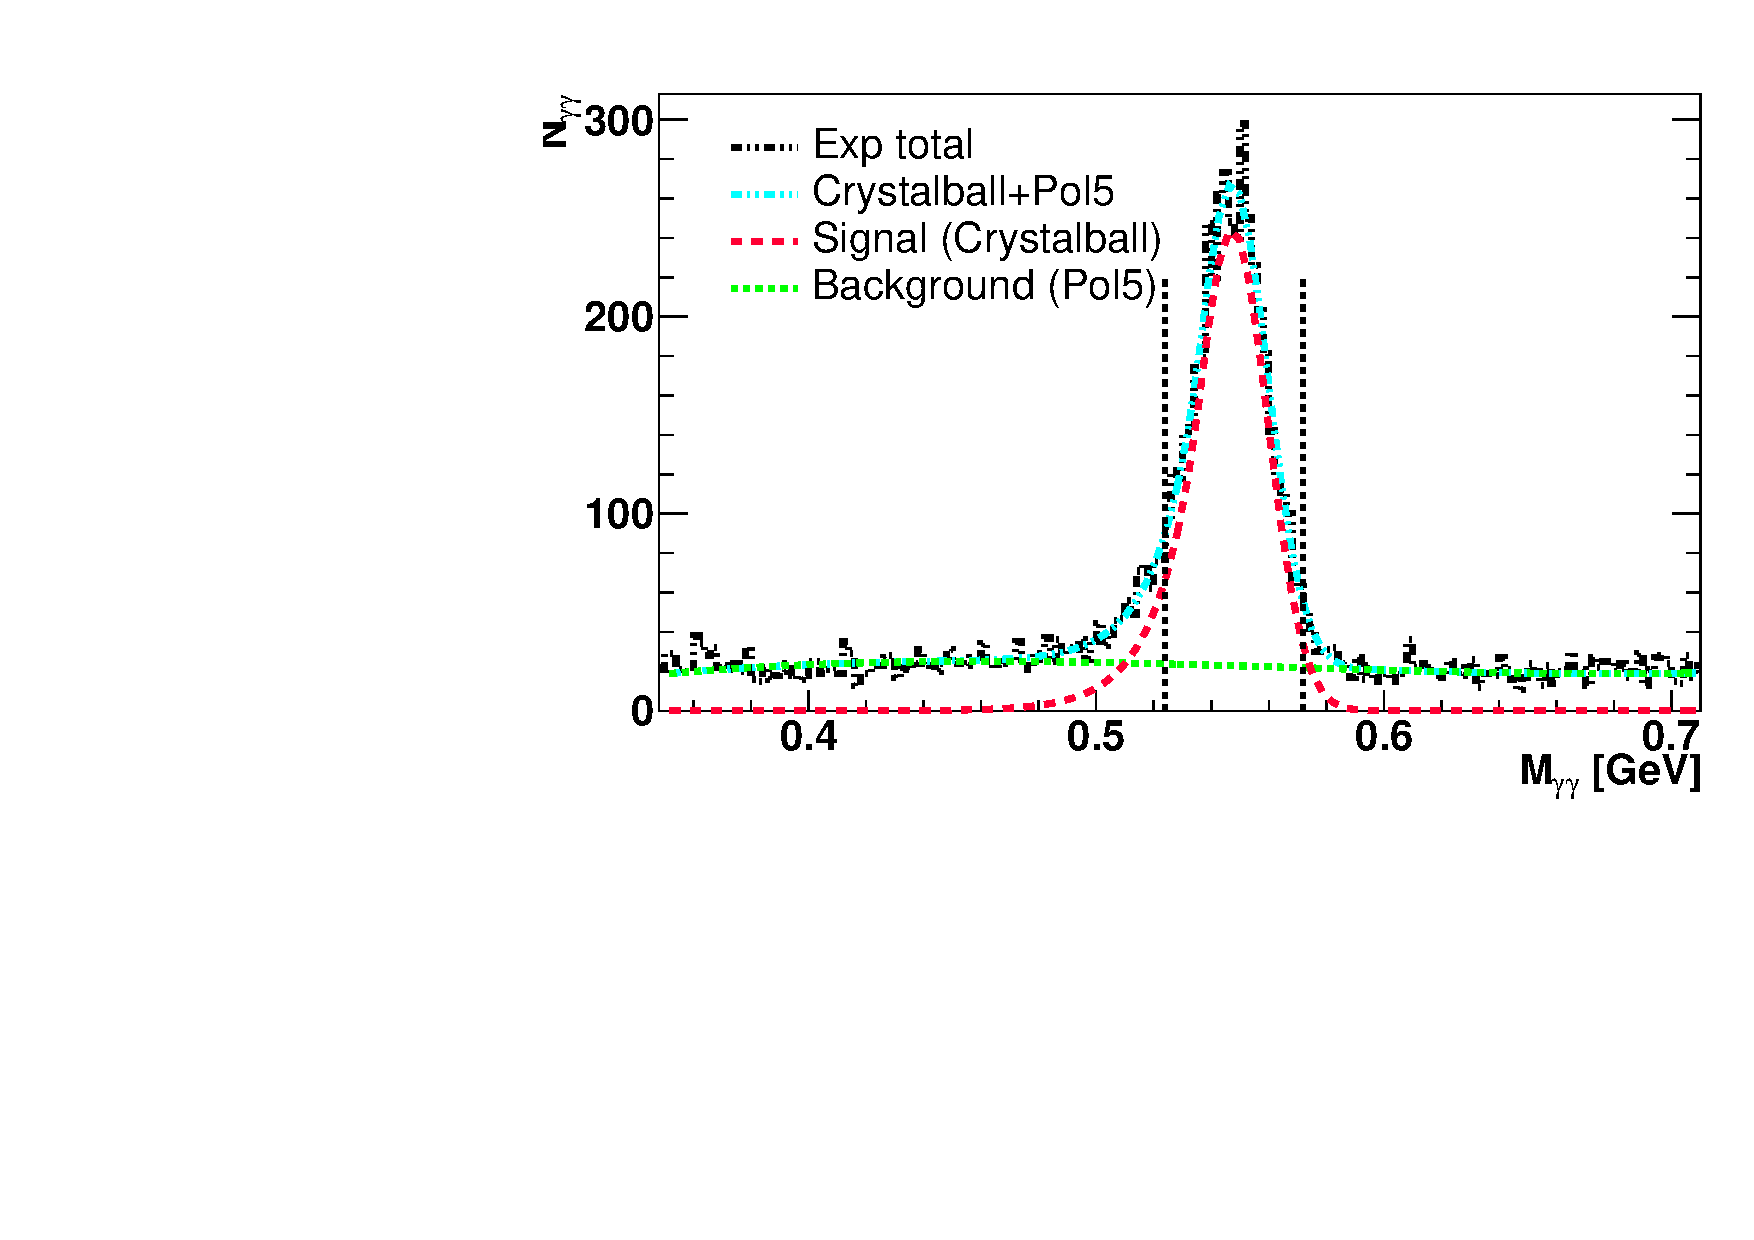
\includegraphics[width=.48\textwidth,natwidth=600,natheight=400]{figure_dataselection/eta_fitall_Z_6.pdf}}
 \subfigure[$z$ bin 6, $0.6<z<0.7$]{\label{fig:etafitz62}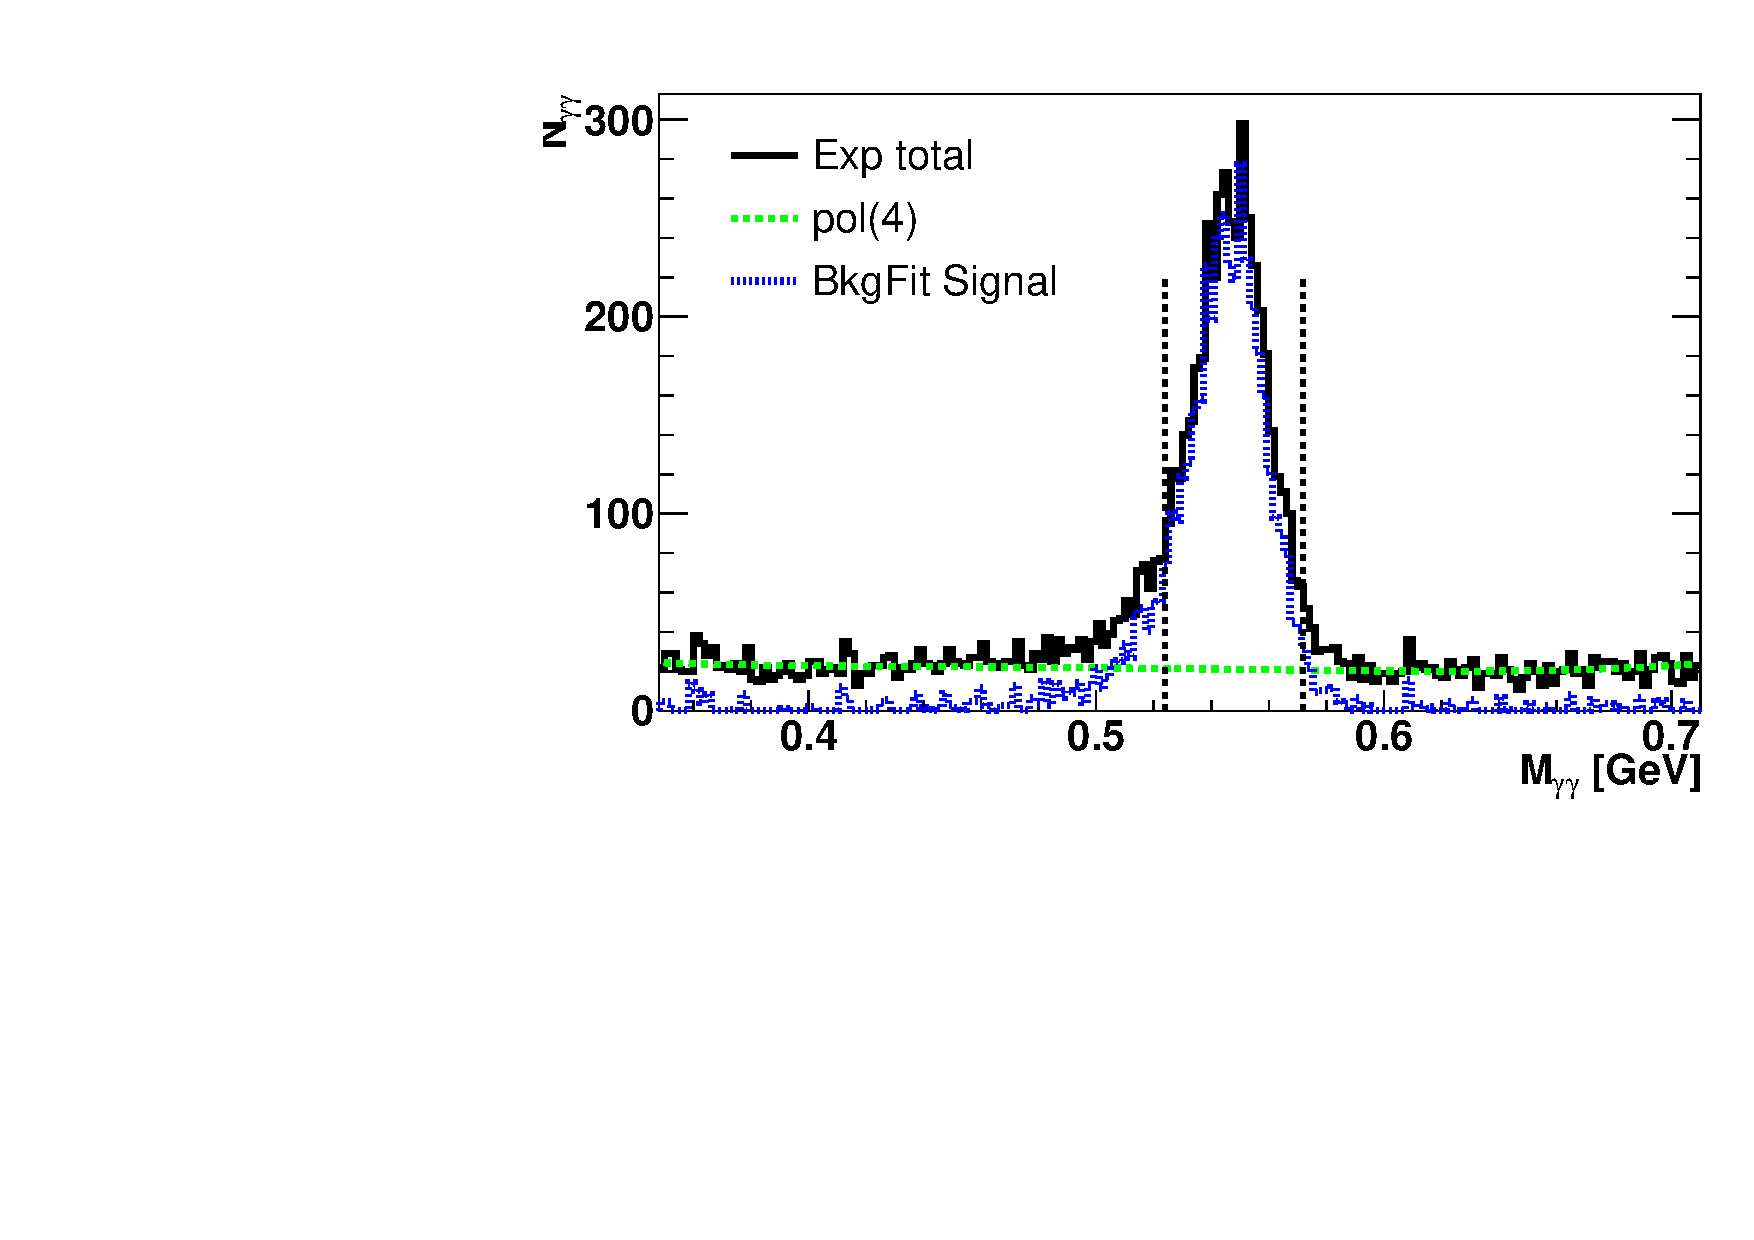
\includegraphics[width=.48\textwidth,natwidth=600,natheight=400]{figure_dataselection/eta_fitbkg_Z_6.pdf}}
\label{fig:etazfit}
\caption{}
\end{figure}

\begin{figure}[H]
 \ContinuedFloat 
  \centering
  \subfigure[$P_t$ bin 1, $0<p_t<0.15$]{\label{fig:etafitpt0}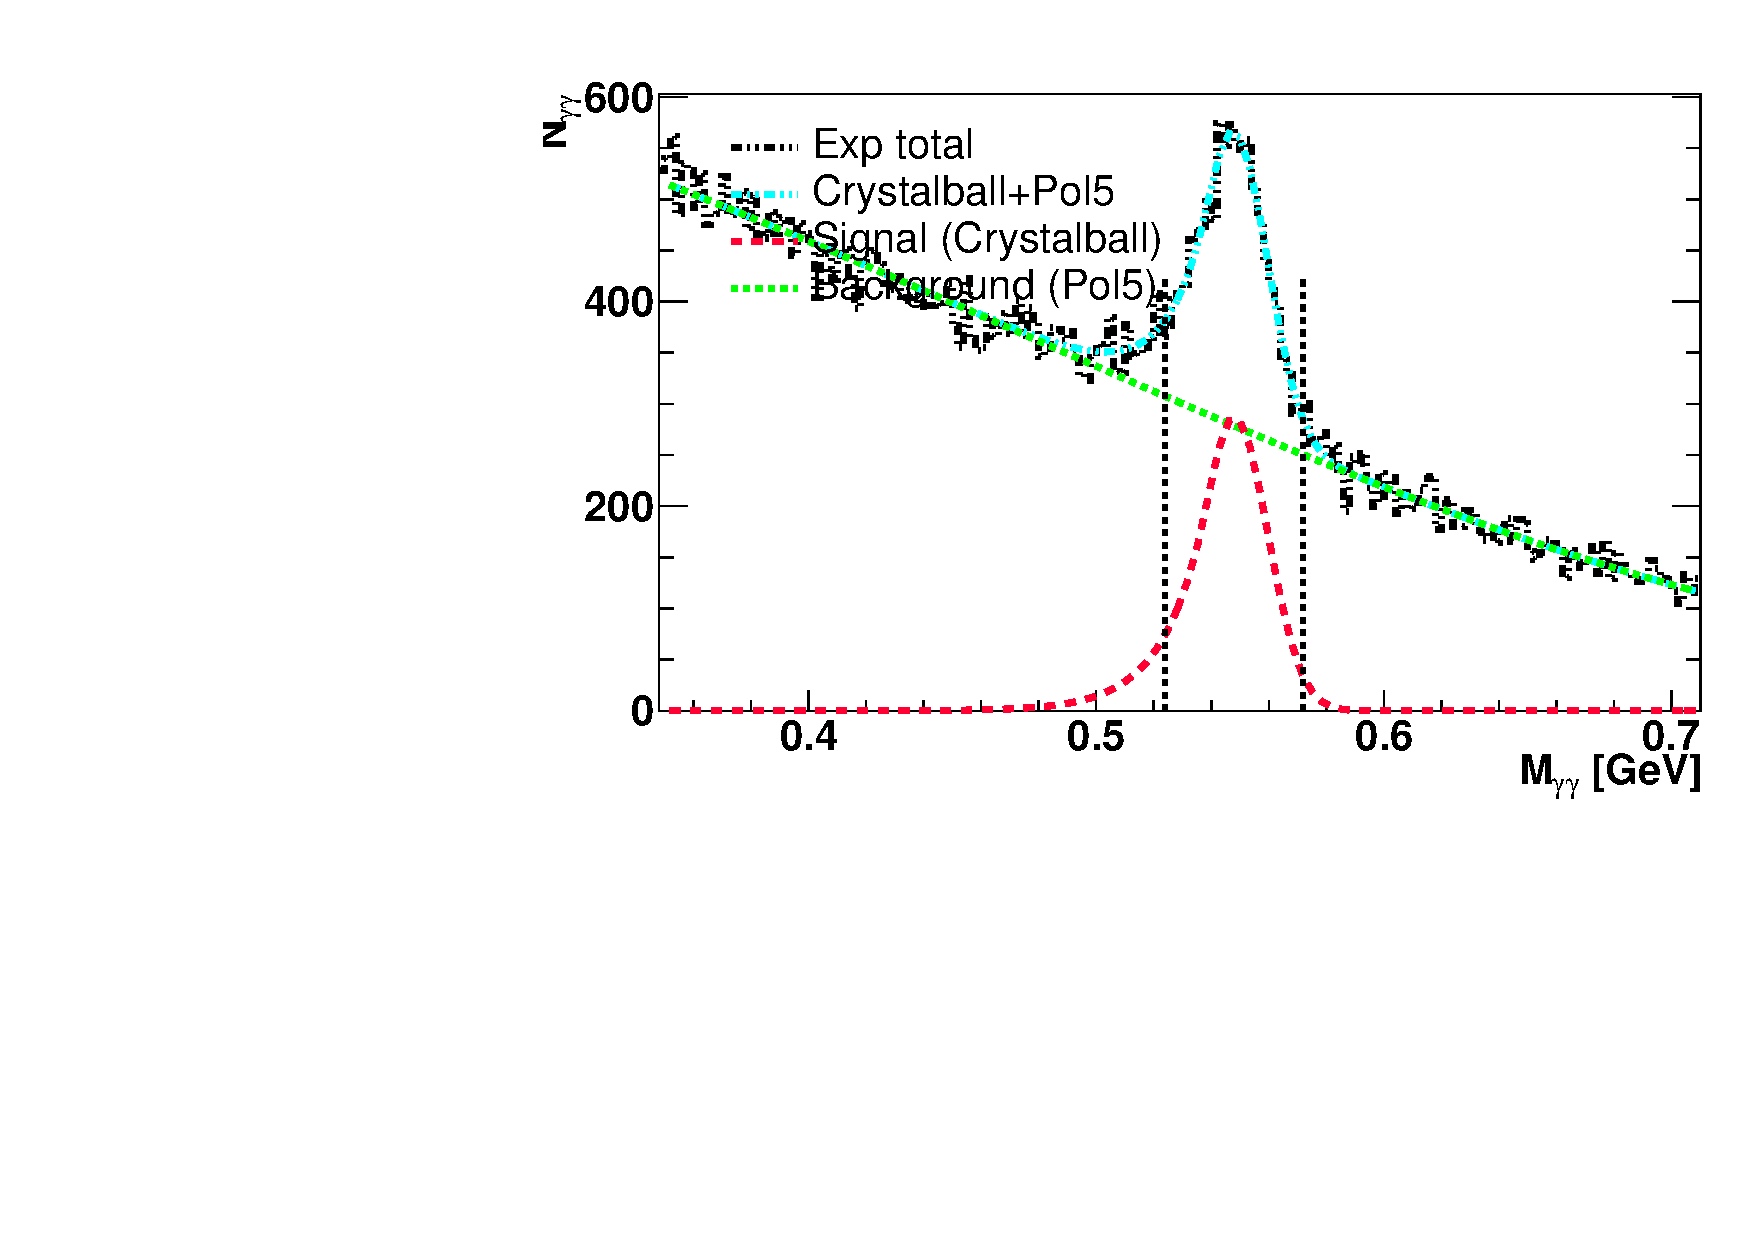
\includegraphics[width=.48\textwidth,natwidth=600,natheight=400]{figure_dataselection/eta_fitall_Pt_0.pdf}}
 \subfigure[$P_t$ bin 1, $0<p_t<0.15$]{\label{fig:etafitpt02}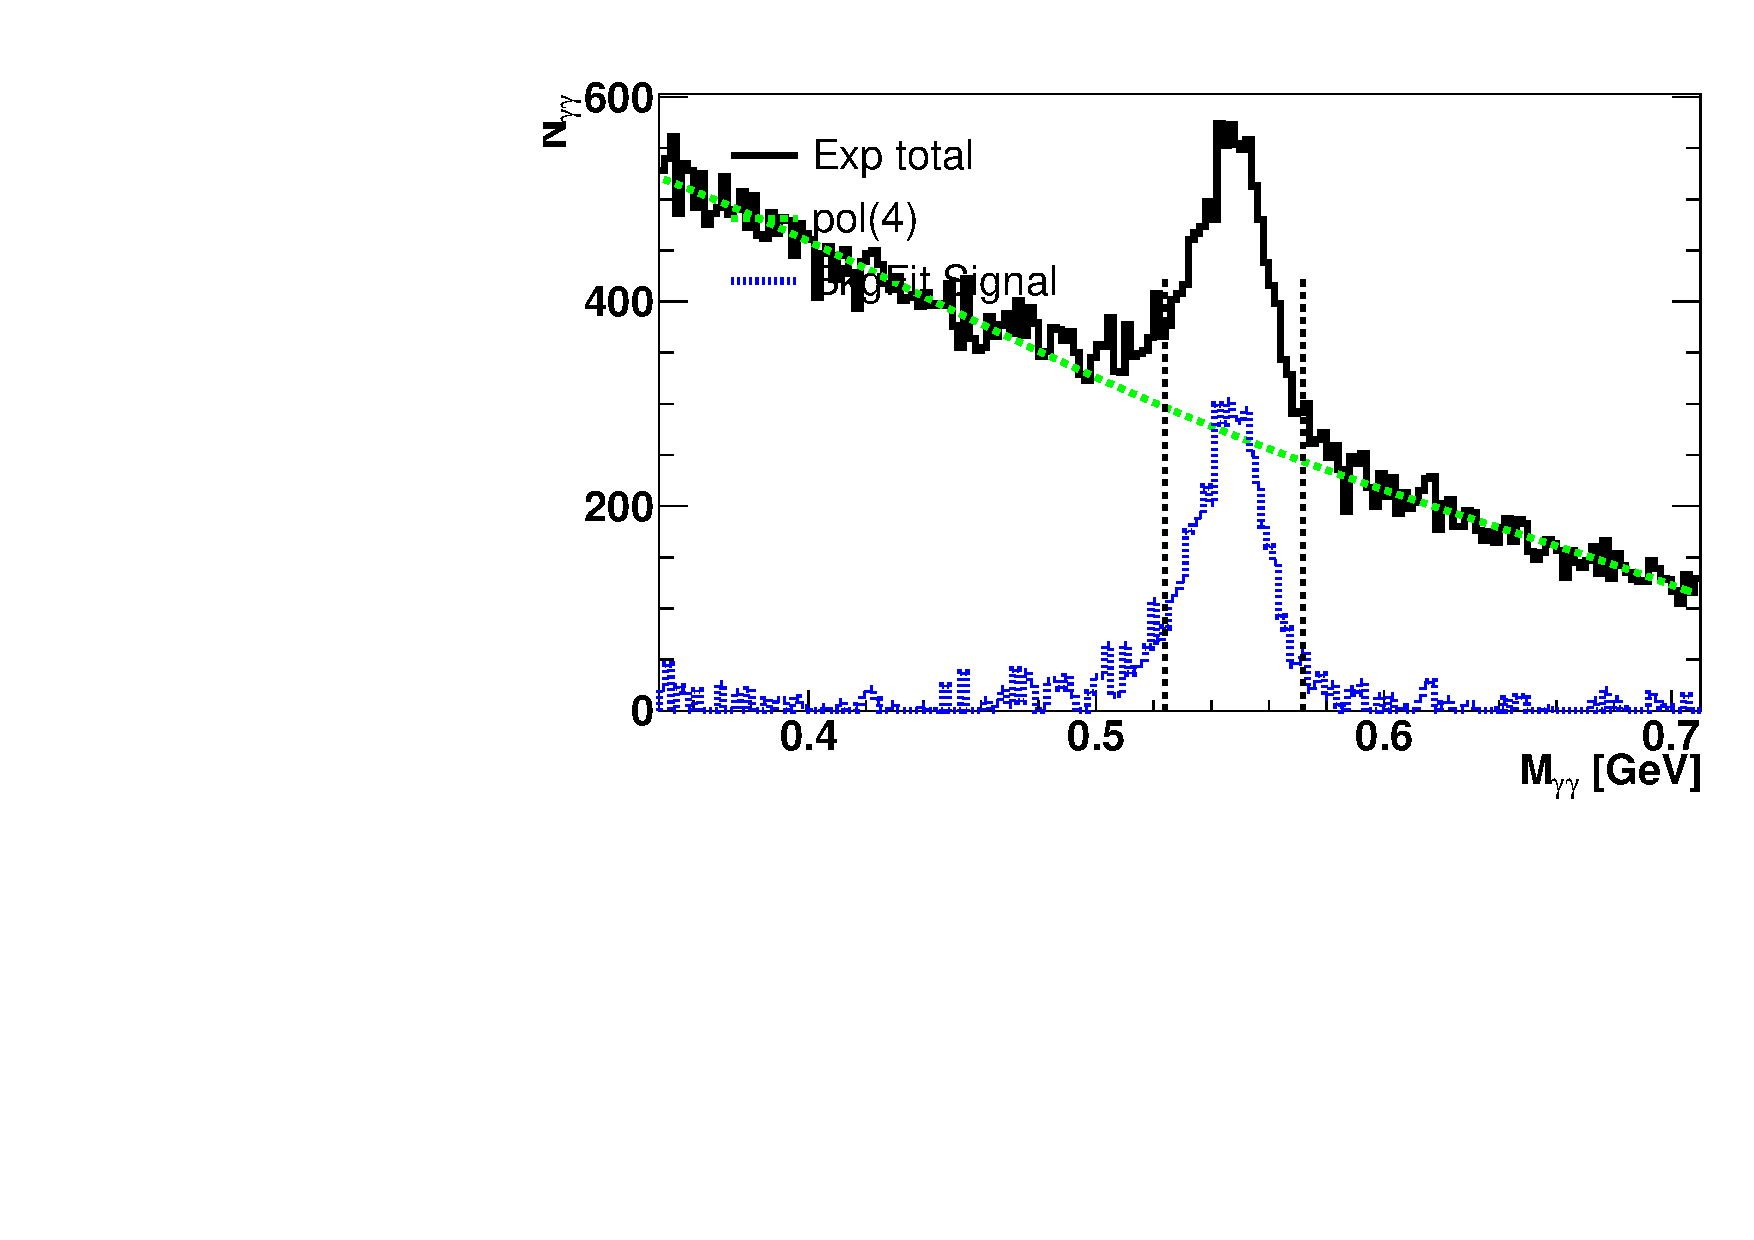
\includegraphics[width=.48\textwidth,natwidth=600,natheight=400]{figure_dataselection/eta_fitbkg_Pt_0.pdf}}
  \subfigure[$P_t$ bin 2, $0.15<p_t<0.3$]{\label{fig:etafitpt1}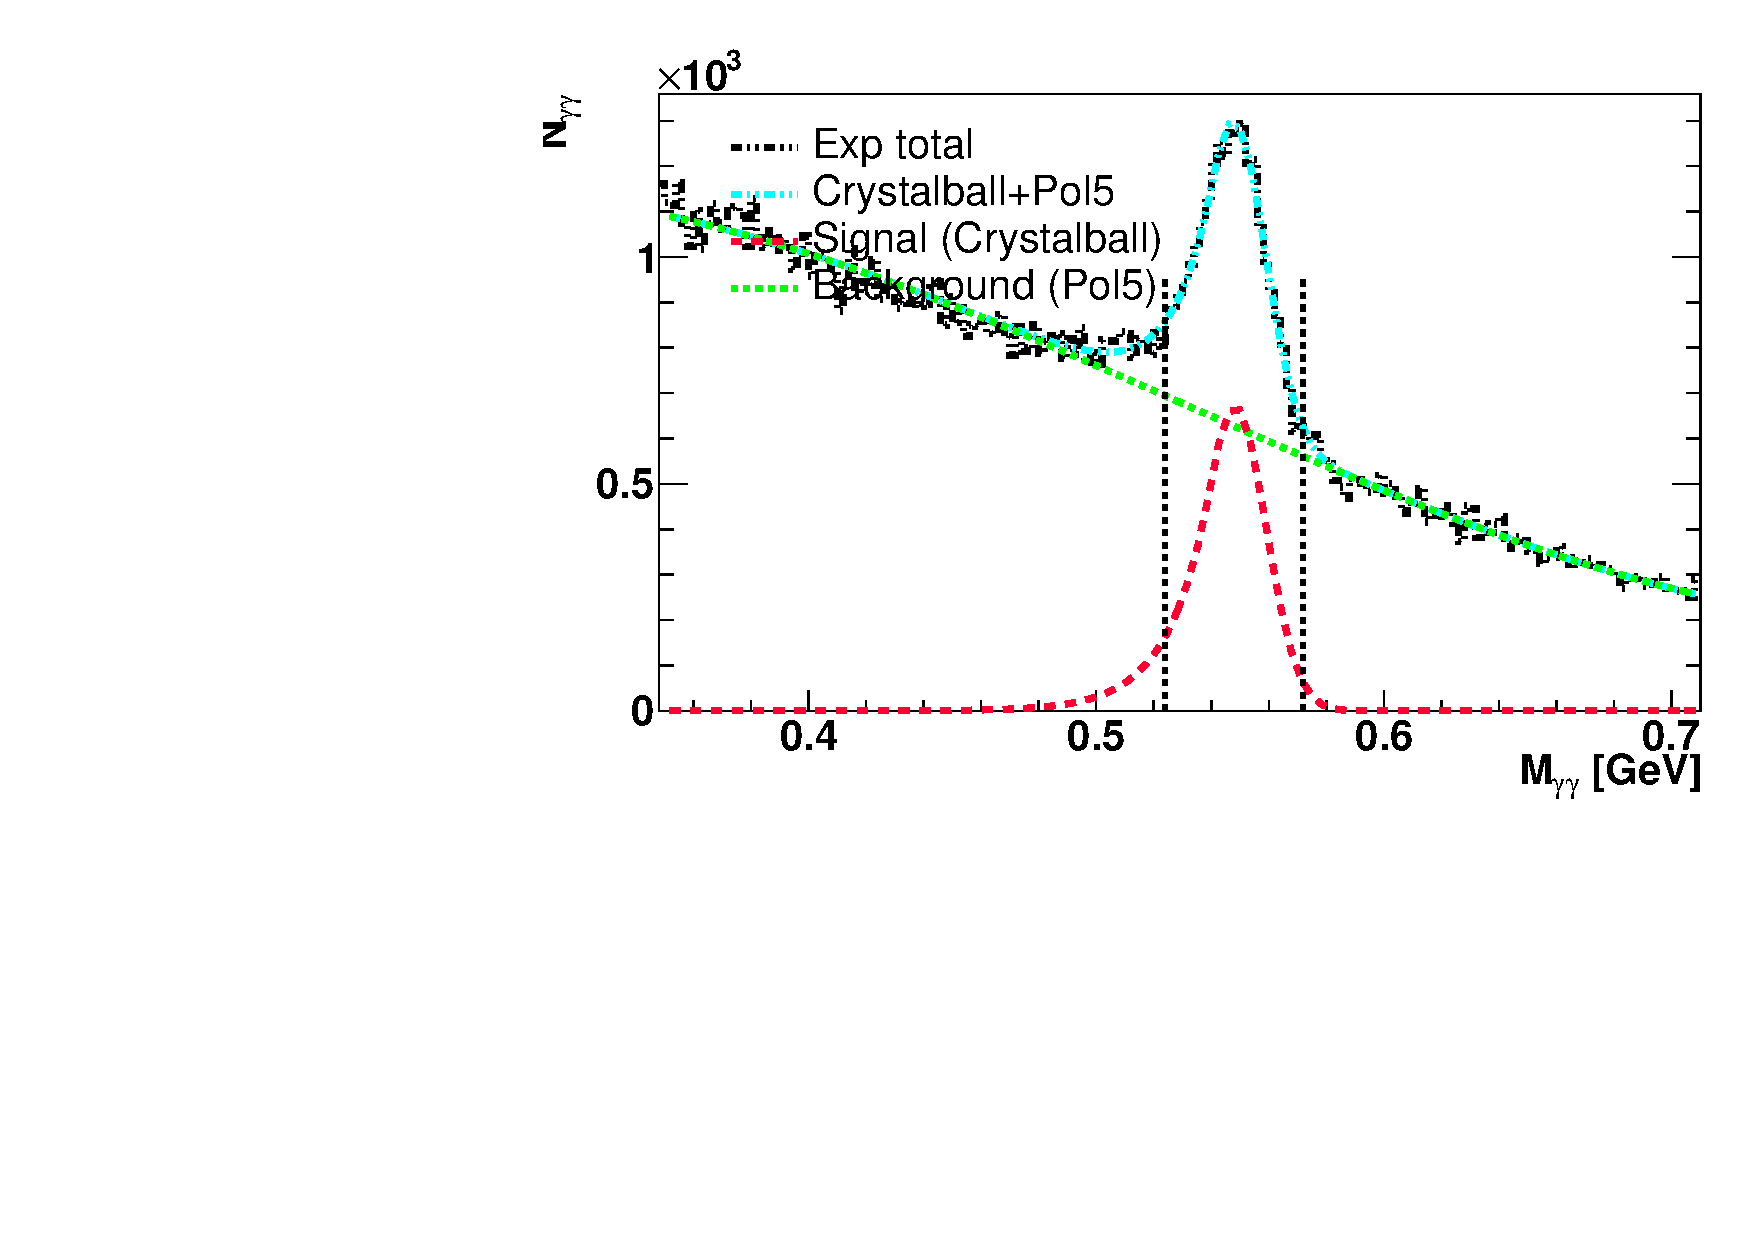
\includegraphics[width=.48\textwidth,natwidth=600,natheight=400]{figure_dataselection/eta_fitall_Pt_1.pdf}}
 \subfigure[$P_t$ bin 2, $0.15<p_t<0.3$]{\label{fig:etafitpt12}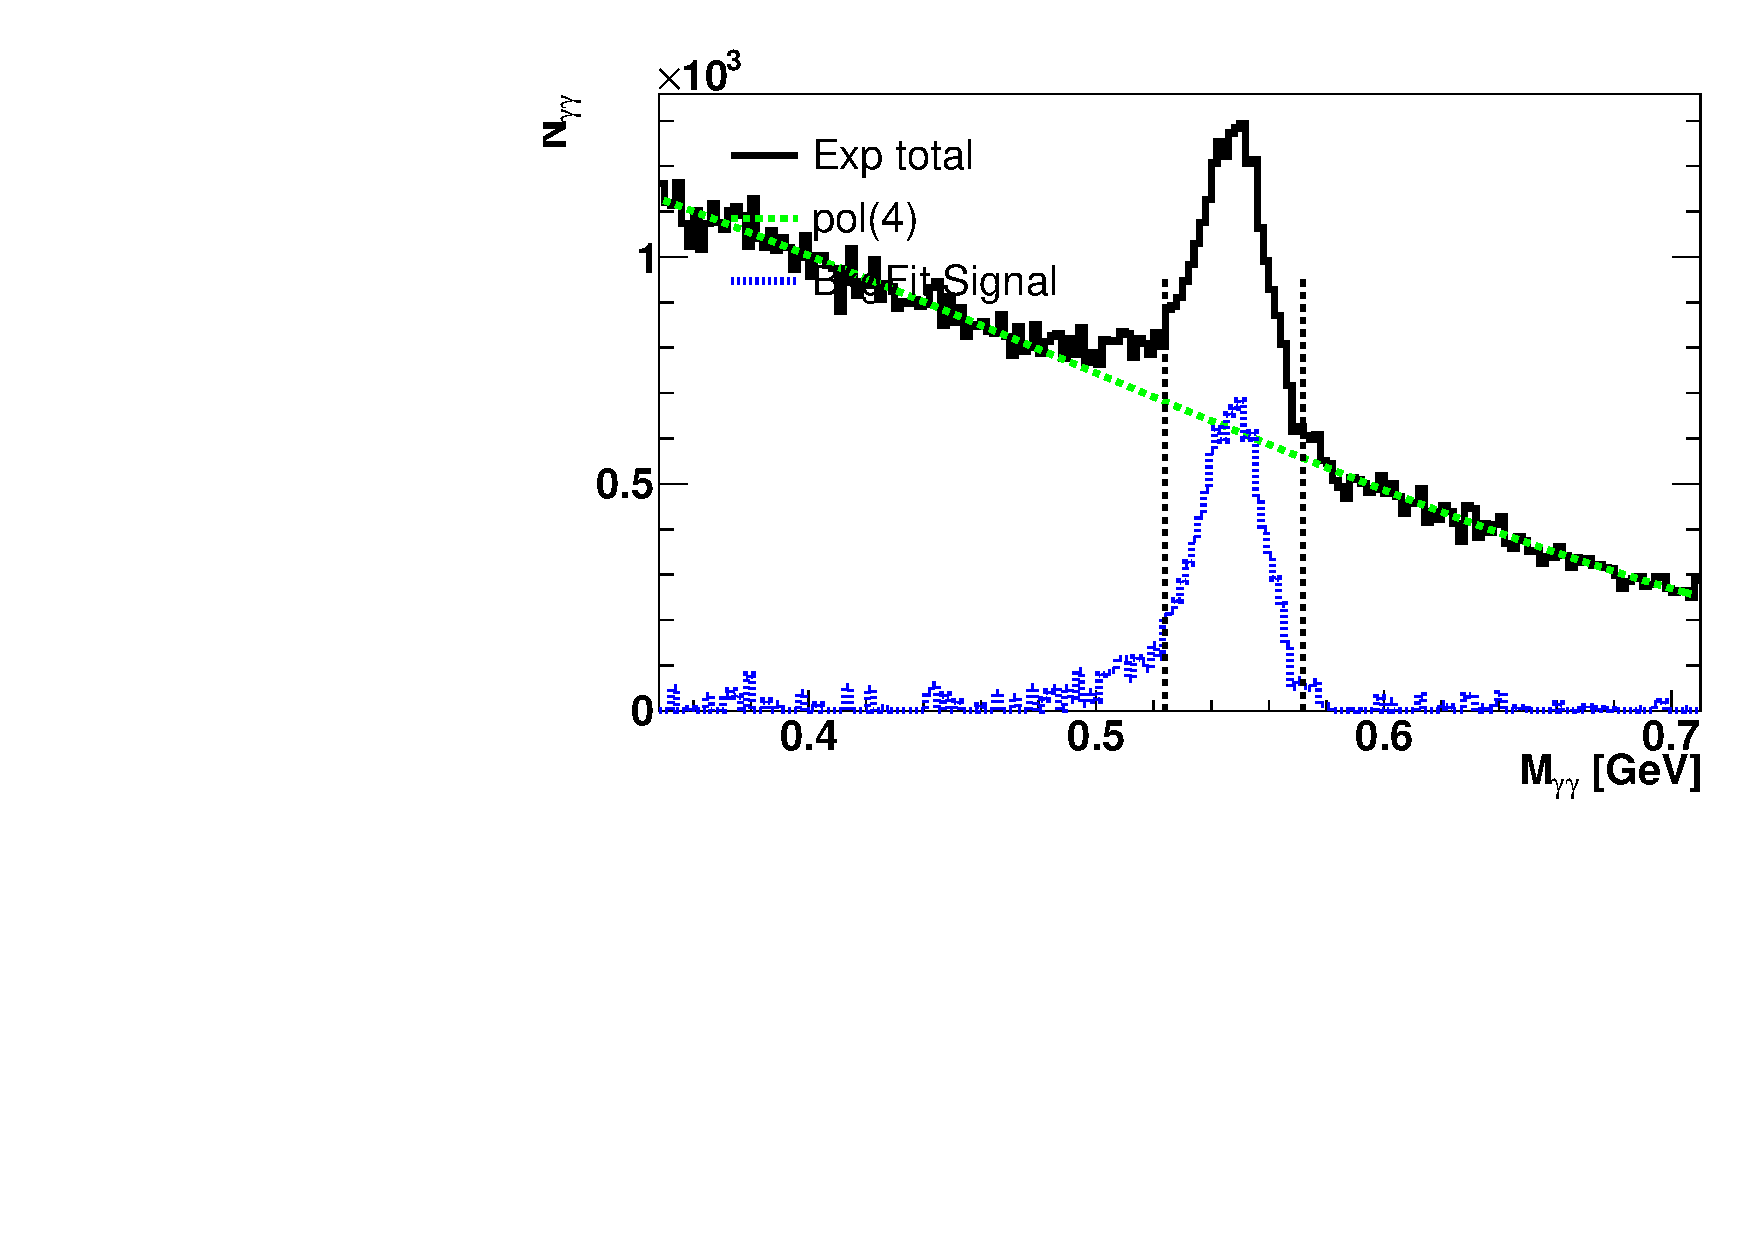
\includegraphics[width=.48\textwidth,natwidth=600,natheight=400]{figure_dataselection/eta_fitbkg_Pt_1.pdf}}
  \subfigure[$P_t$ bin 3, $0.3<p_t<0.5$]{\label{fig:etafitpt2}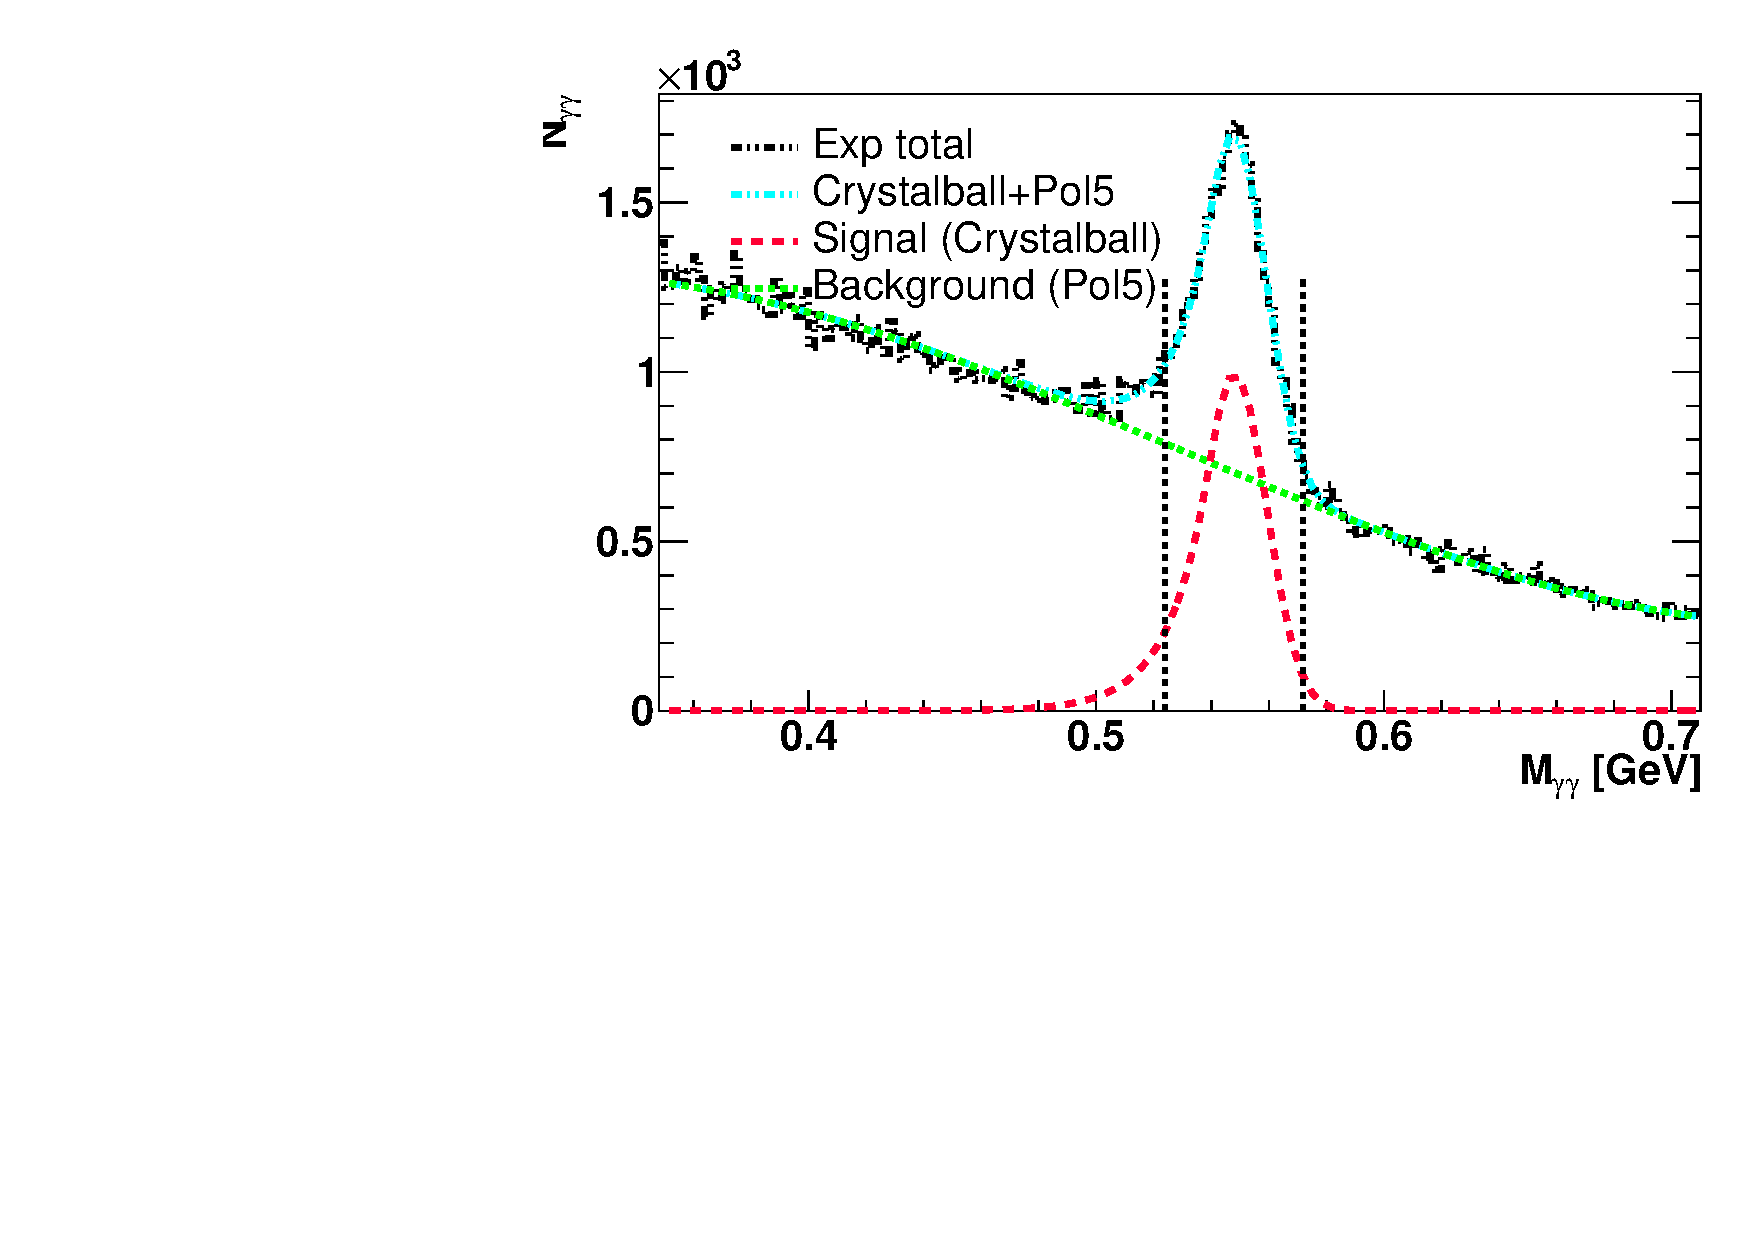
\includegraphics[width=.48\textwidth,natwidth=600,natheight=400]{figure_dataselection/eta_fitall_Pt_2.pdf}}
\subfigure[$P_t$ bin 3, $0.3<p_t<0.5$]{\label{fig:etafitpt22}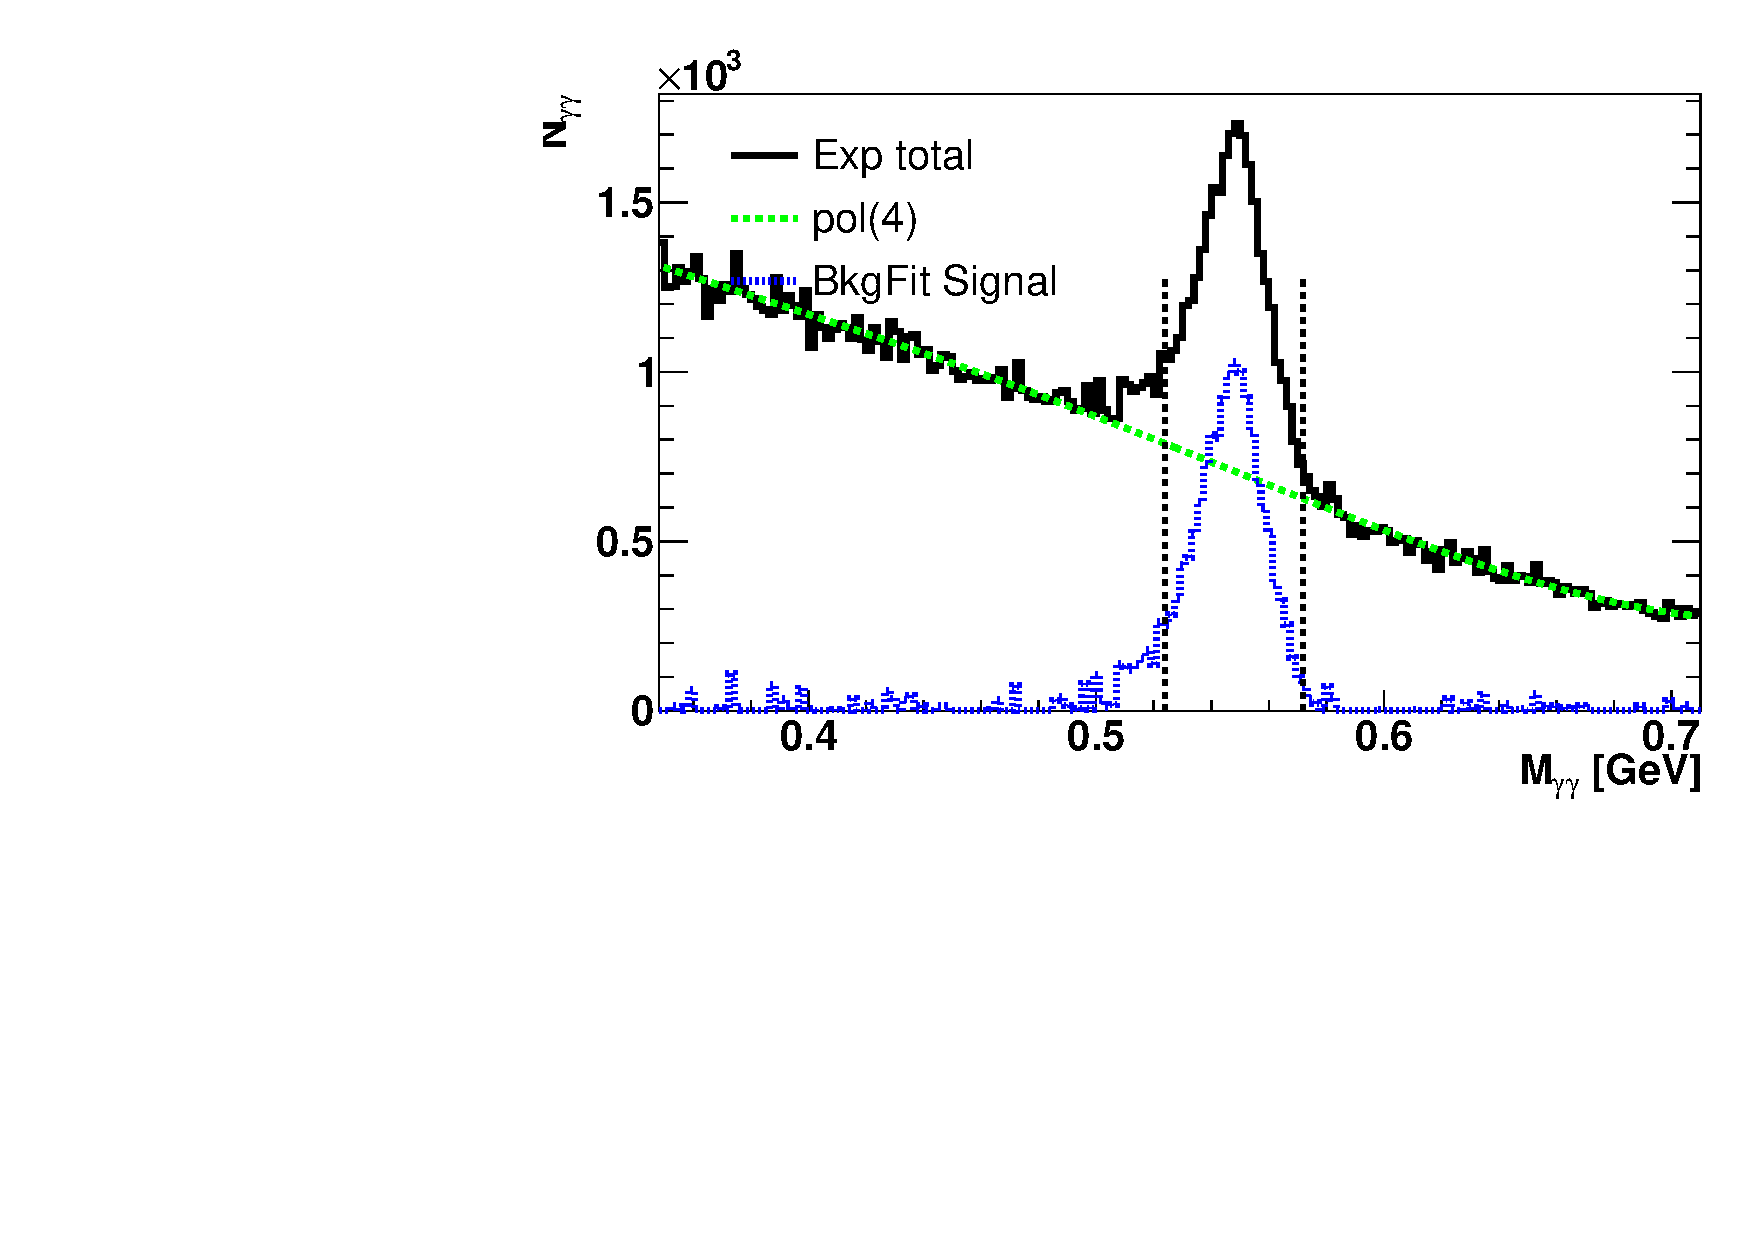
\includegraphics[width=.48\textwidth,natwidth=600,natheight=400]{figure_dataselection/eta_fitbkg_Pt_2.pdf}}
  \subfigure[$P_t$ bin 4, $0.5<p_t<3$]{\label{fig:etafitpt3}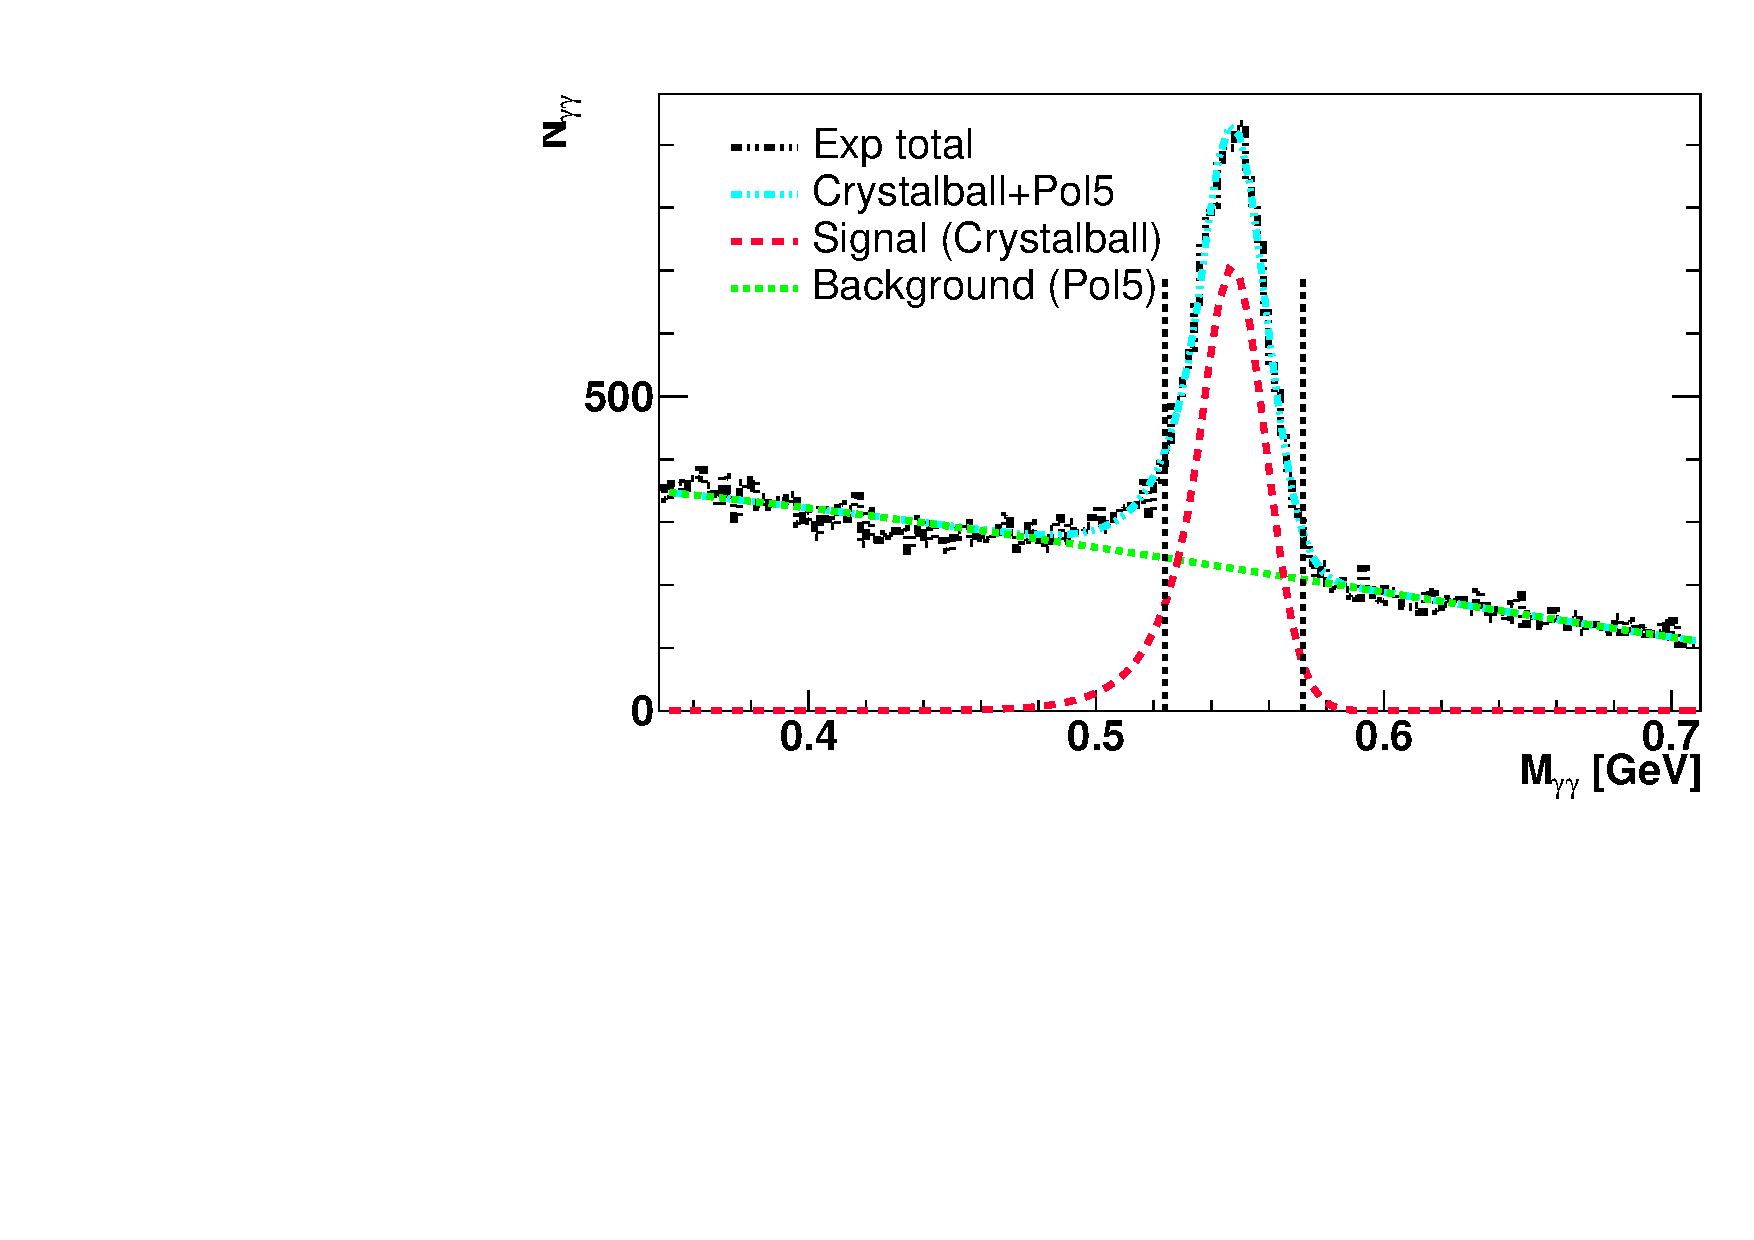
\includegraphics[width=.48\textwidth,natwidth=600,natheight=400]{figure_dataselection/eta_fitall_Pt_3.pdf}}
\subfigure[$P_t$ bin 4, $0.5<p_t<3$]{\label{fig:etafitpt32}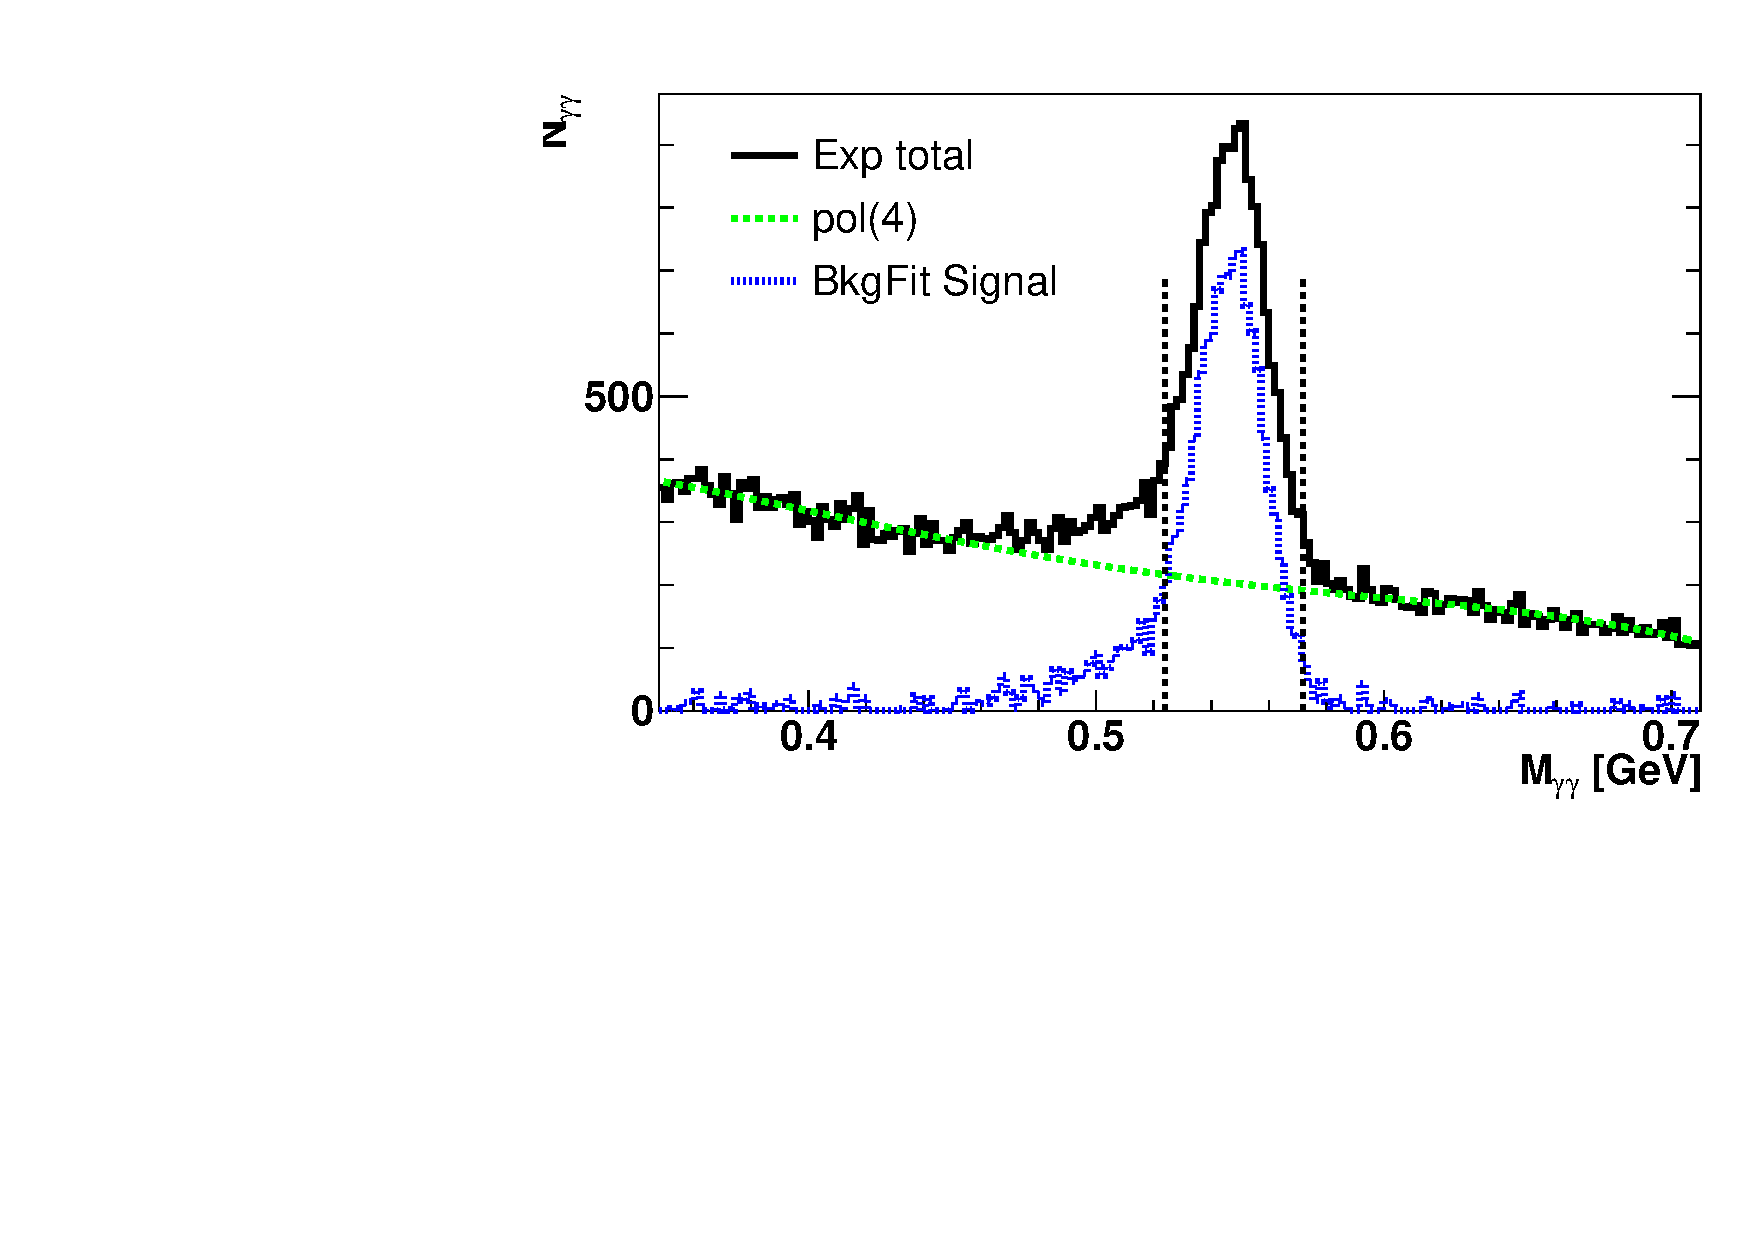
\includegraphics[width=.48\textwidth,natwidth=600,natheight=400]{figure_dataselection/eta_fitbkg_Pt_3.pdf}}
  \caption{$\eta$ fit results for all kinematic bins. Fit method has described in section~\ref{sec:etafitsection}. In the left row the red line is the background and green line is the signal. In the right row only background is fitted using polynomial function~(green line), and the signal~(blue dash line) is obtained by subtracting the background from total data.}
  \label{fig:etaptfit}
\end{figure}
